\thispagestyle{hoccungpinone}
\pagestyle{hoccungpi}
\everymath{\color{hoccungpi}}
\graphicspath{{../hoccungpi/pic/}}
\blfootnote{$^{1}$\color[named]{diendantoanhoc}THPT chuyên Lê Quý Đôn, Bình Định.}
\begingroup
\AddToShipoutPicture*{\put(0,616){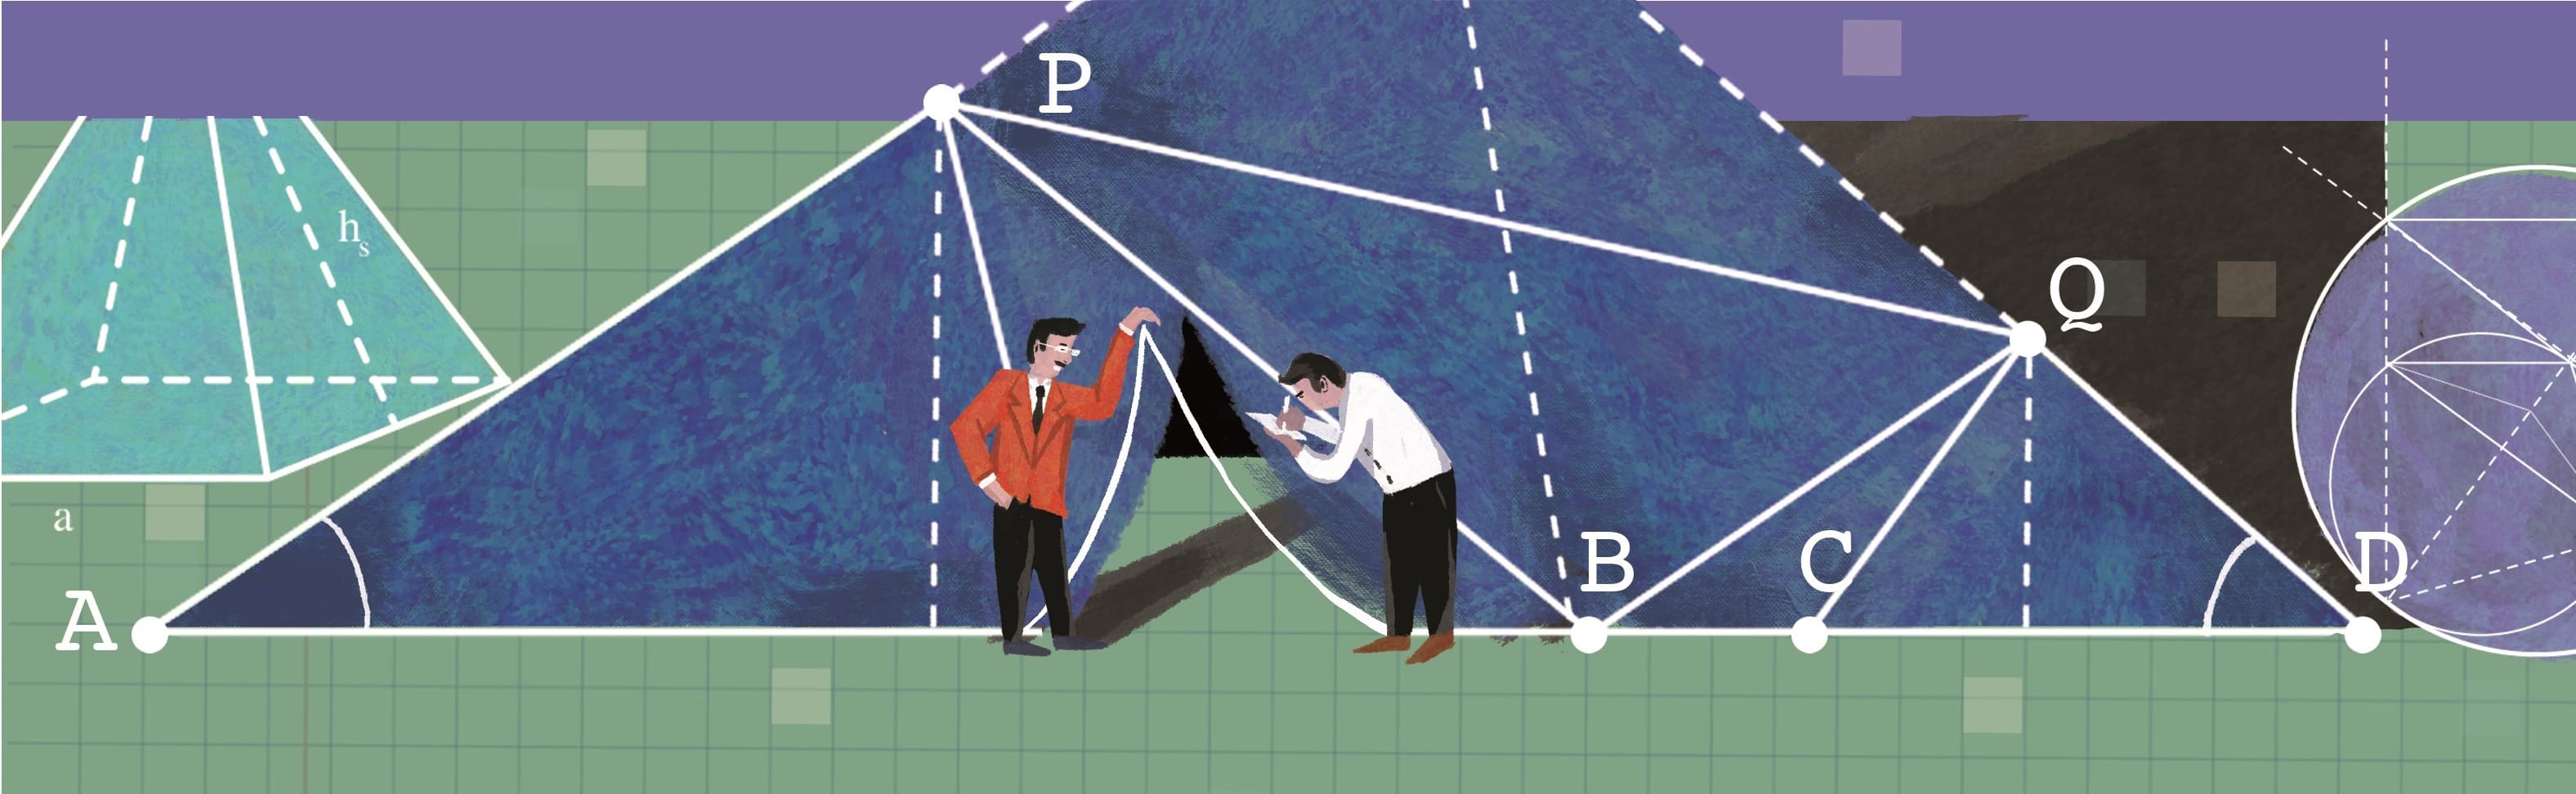
\includegraphics[width=19.3cm]{../bannerhoccungpi}}}
\AddToShipoutPicture*{\put(124,525){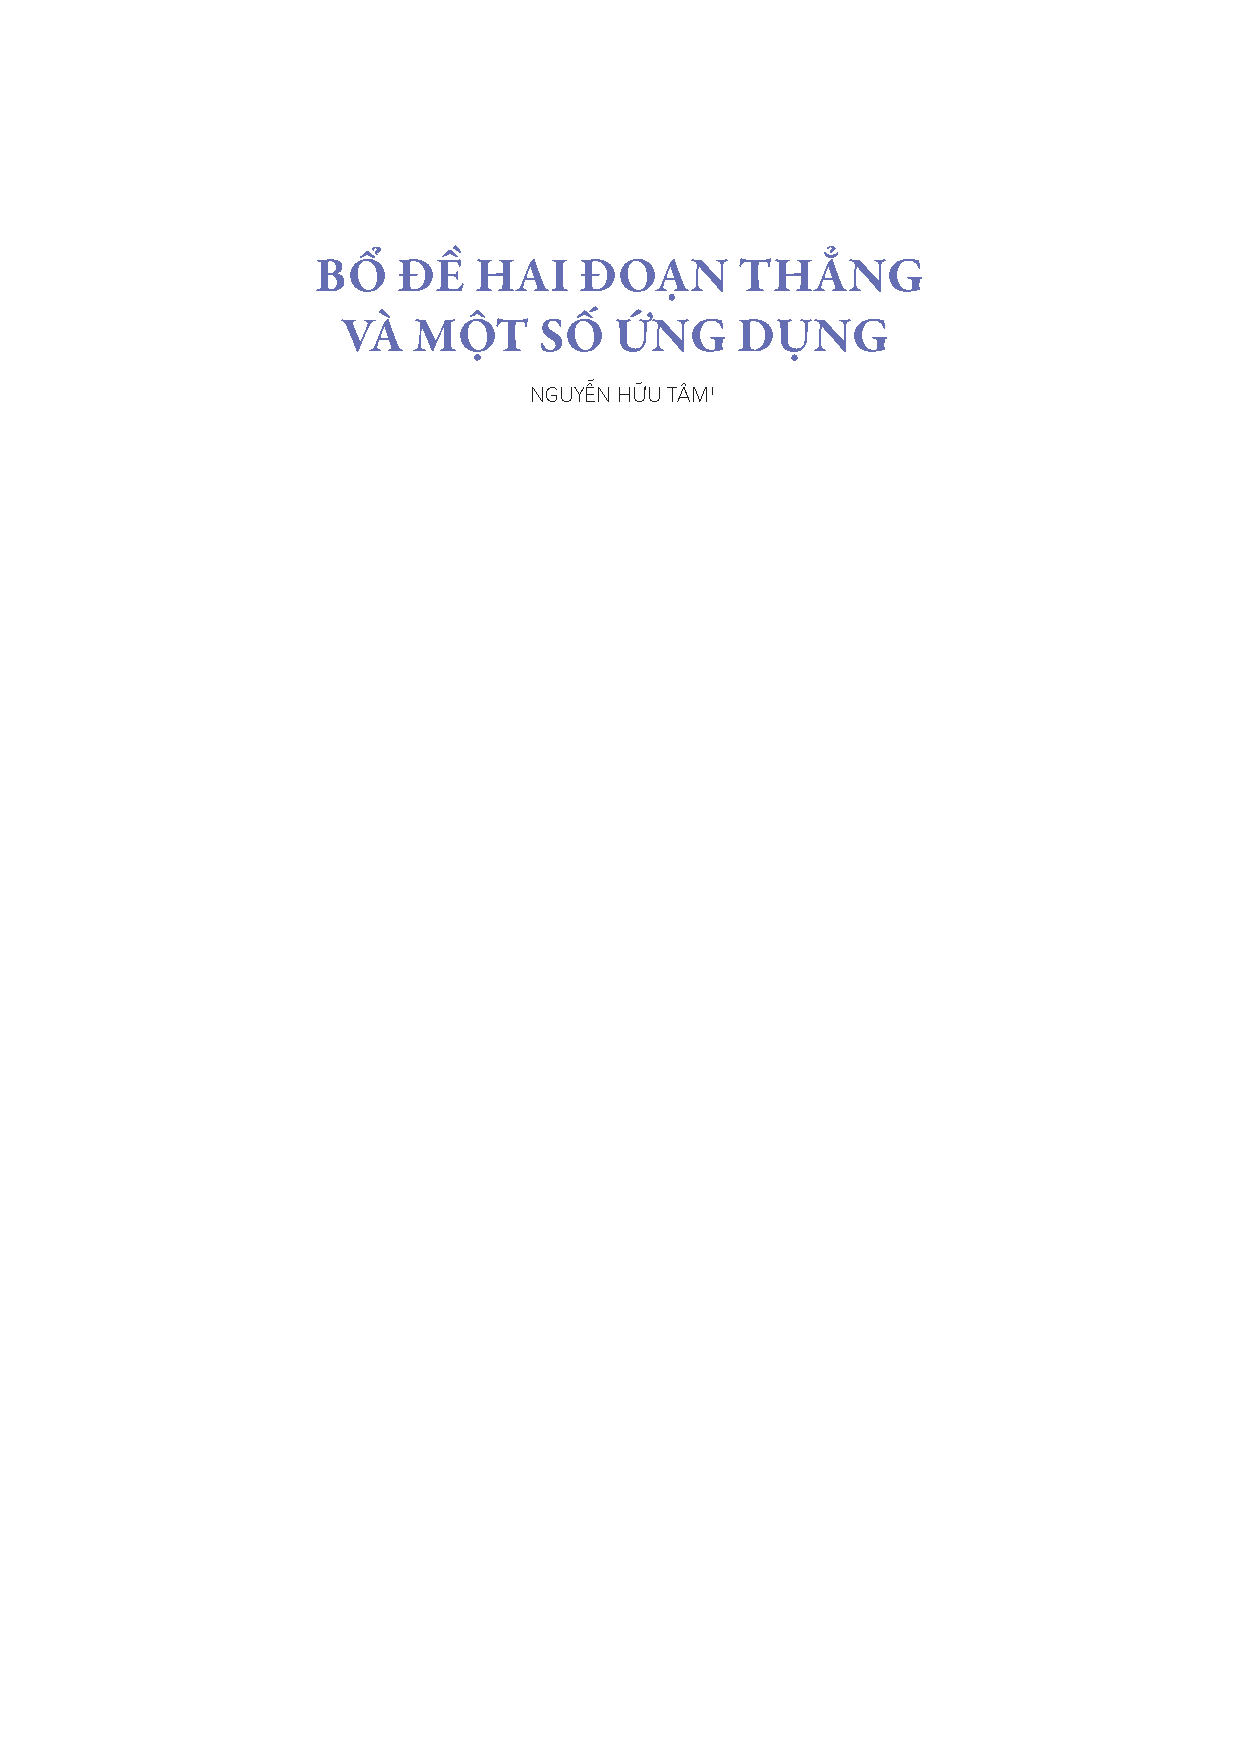
\includegraphics[scale=1]{../tieude1.pdf}}}
\centering
\endgroup

\vspace*{192pt}

\textit{\textbf{\color{hoccungpi}LTS.} Kỳ thi Bài giảng và bài viết về Toán học, lần thứ $2$, năm $2023$, do Tạp chí Pi tổ chức, với sự phối hợp của Hội Toán học, Viện Hàn lâm Khoa học và Công nghệ Việt Nam, là một diễn đàn dành cho độc giả của Pi và những người yêu Toán nói chung. Kỳ thi đã nhận được nhiều bài viết có chất lượng chuyên môn cao. Tạp chí Pi số này xin trân trọng giới thiệu cùng bạn đọc bài viết được trao giải Nhất trong hạng mục Chuyên đề Toán học.}
\begin{multicols}{2}
	Bài viết này trình bày về hai bổ đề liên quan đến mô hình hai đoạn thẳng và một vài ứng dụng trong việc tiếp cận, khai thác một số bài toán hình học phẳng.
	\vskip 0.1cm
	\textbf{\color{hoccungpi}$\pmb{1.}$ Bổ đề về hai đoạn thẳng} 
	\vskip 0.1cm
	Trong các bài toán hình học phẳng, chúng ta khá thường xuyên gặp tình huống có hai đoạn thẳng bằng nhau. Điều đó có thể gợi đến kết quả sau đây, mà chúng tôi tạm gọi là \textit{Bổ đề hai đoạn thẳng}.
	\vskip 0.1cm 
	\textbf{\color{hoccungpi}Bổ đề $\pmb{1.}$} Cho hai đoạn thẳng $AB$ và $A'B'$ trong mặt phẳng sao cho $AB$ không cùng phương với $A'B'$ và $AB=A'B'$. Khi đó tồn tại một phép quay biến $A$ thành $A'$ và $B$ thành $B'$. đồng thời cũng tồn tại một phép quay biến $A$ thành $B'$ và biến $B$ thành $A'$.
	\vskip 0.1cm
	Trước khi đi vào chứng minh, bạn đọc có thể nhận thấy rằng, bằng cách đổi vai trò của $A'$ và $B'$, ta suy ra tồn tại phép quay thứ hai biến $A$ thành $B'$ và  $B$ thành $A'$.
	\vskip 0.1cm
	\textit{Chứng minh.} Gọi $S$ là giao điểm của $AB$ và $A'B'$. Giả sử các đường trung trực của $AA'$ và $BB'$ cắt nhau tại $T$, dễ thấy hai tam giác $TAB$ và $TA'B'$ bằng nhau (c.c.c). Do đó $(BA,BT)=(B'A',B'T)\,\,\,(\bmod \pi)$, hay $(BS,BT)=(B'S,B'T)\,\,\,(\bmod \pi)$; suy ra bốn điểm $S,T,B,B'$ đồng viên. Tương tự thì bốn điểm $S,T,A,A'$ cũng đồng viên. Rõ ràng phép quay tâm $T$, góc quay $(TA,TA')=(TB,TB')$, biến  $A,B$ tương ứng thành $A',B'$. Trong trường hợp $AA'$ và $BB'$ song song thì từ giả thiết ta có hình thang cân $ABB'A'$. Lúc này $T$ trùng $S$ và ta cũng thu được kết quả như trên.
	\begin{figure}[H]
		\vspace*{-5pt}
		\centering
		\captionsetup{labelformat= empty, justification=centering}
		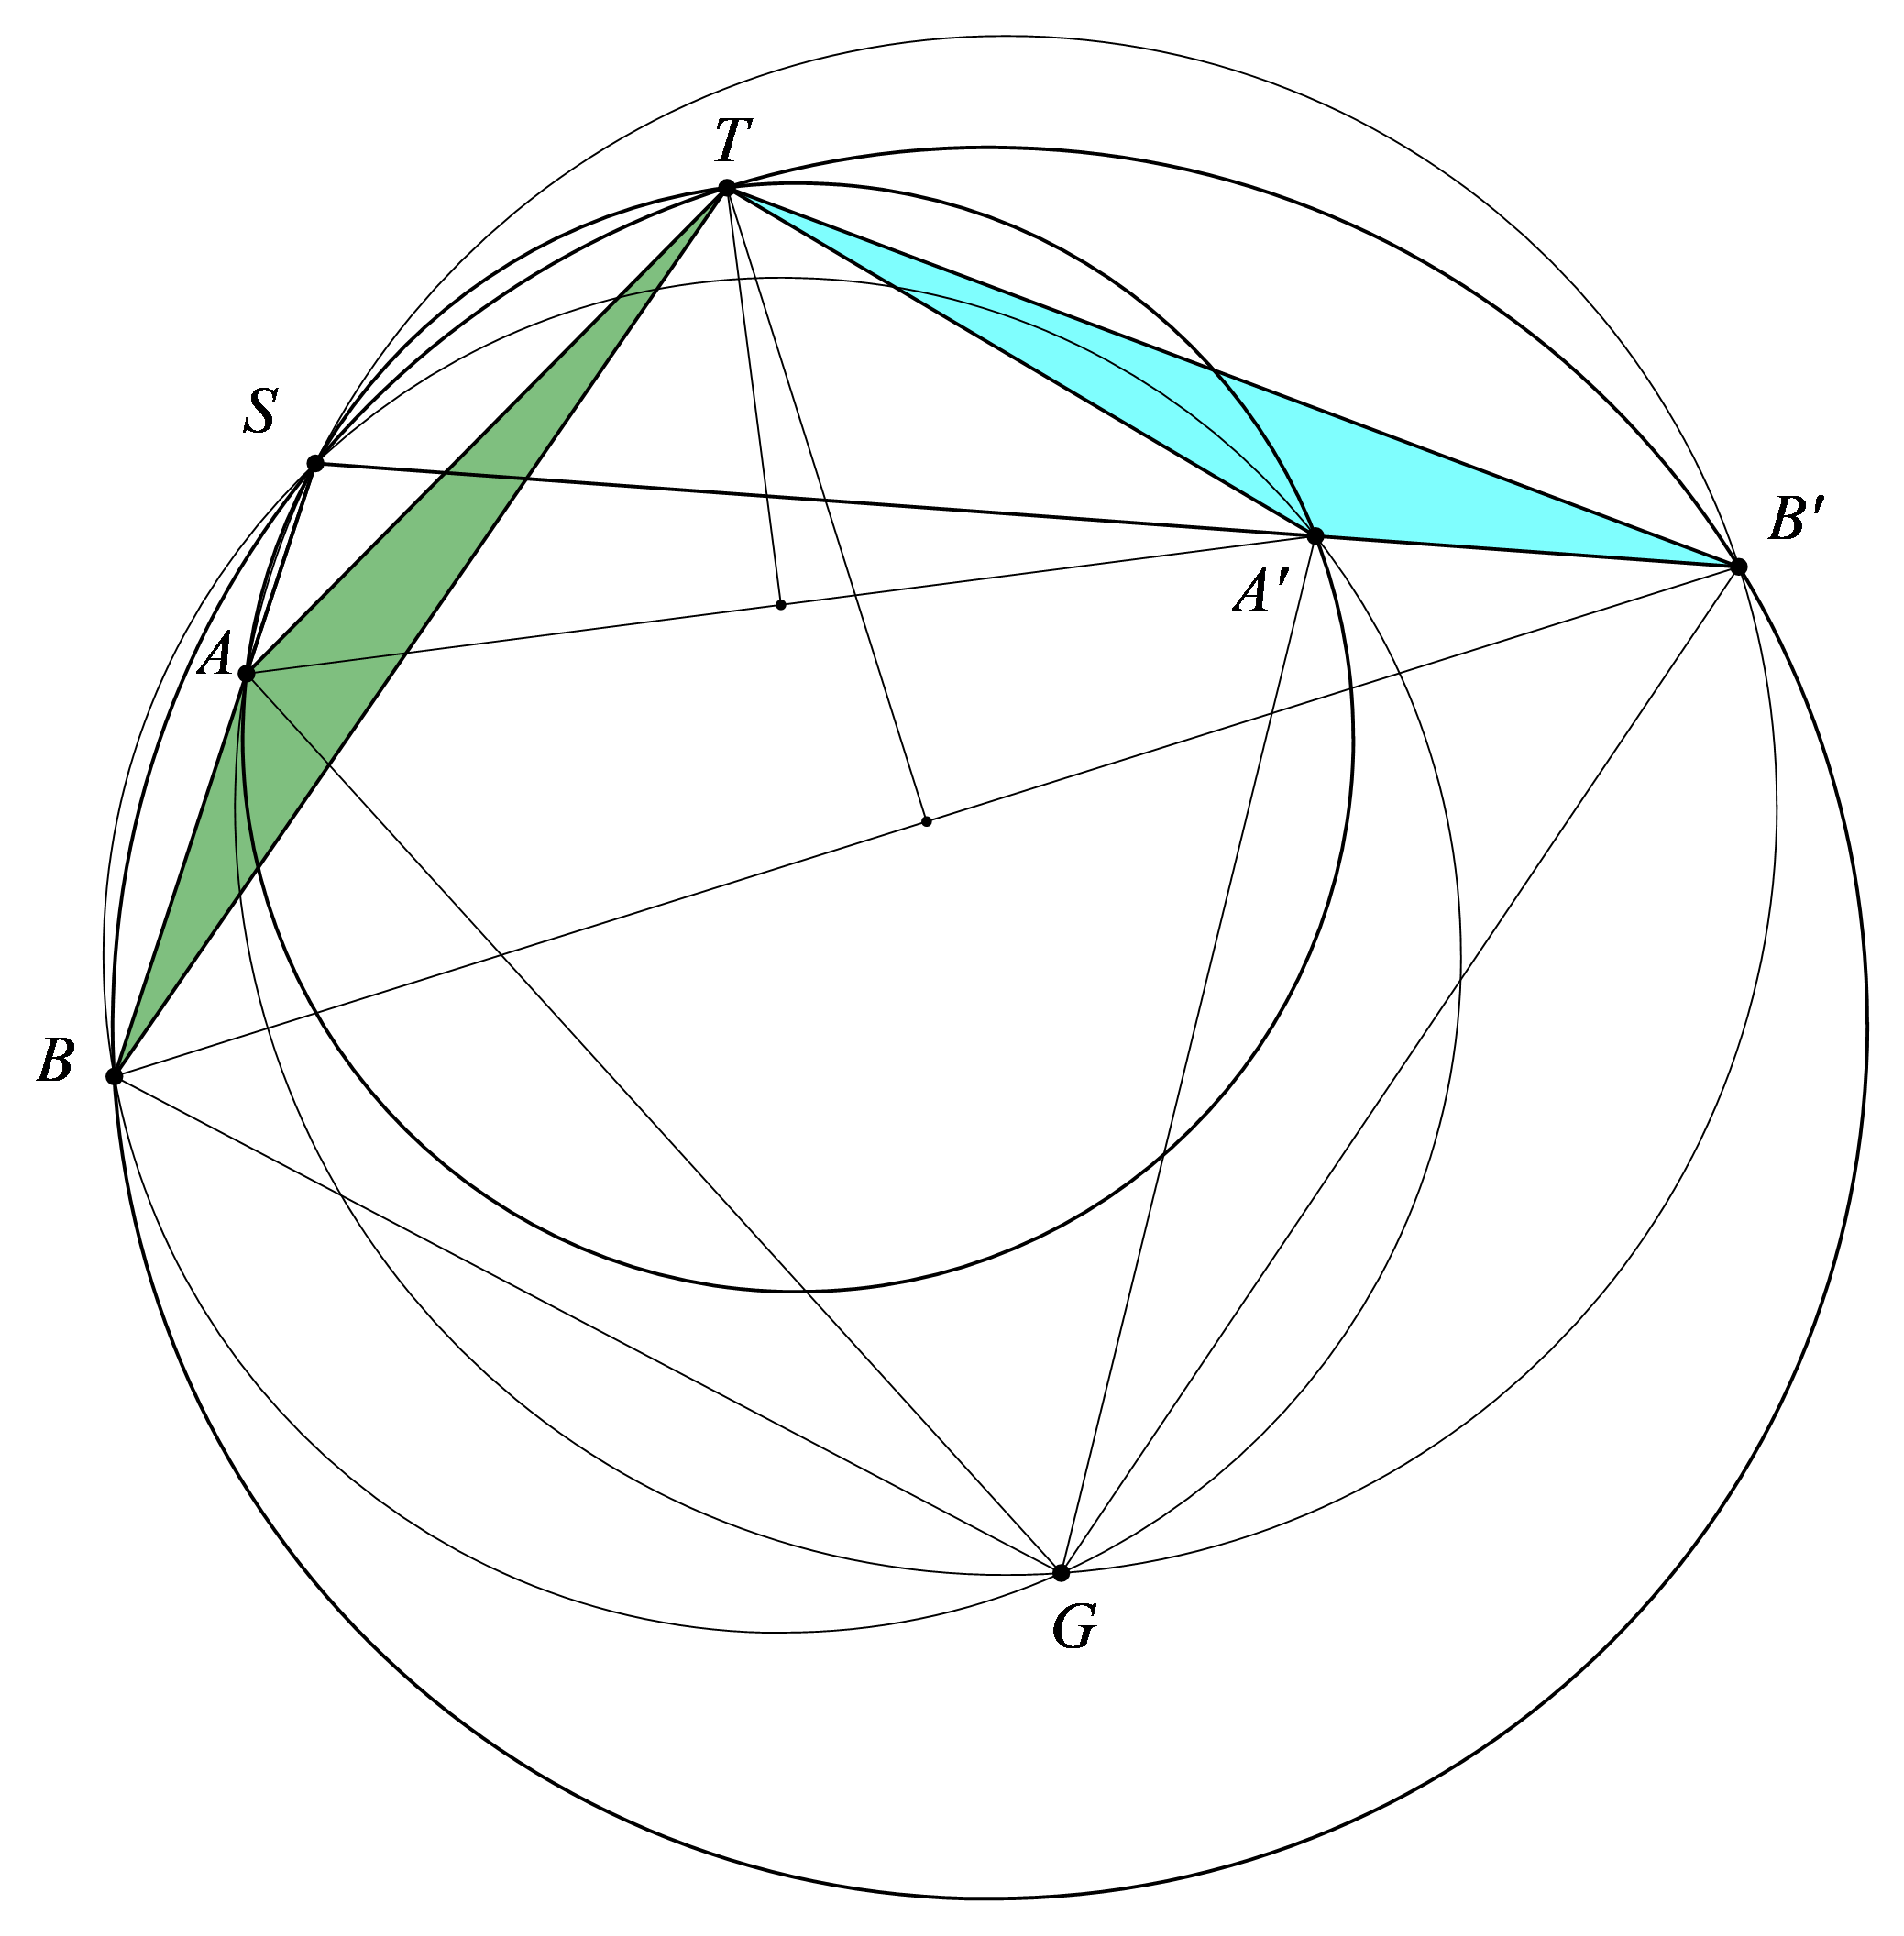
\includegraphics[scale=0.63]{1}
		\vspace*{-5pt}
	\end{figure}
	Chú ý rằng bổ đề trên dẫn đến kết quả sau đây.
	\vskip 0.1cm
	\textbf{\color{hoccungpi}Hệ quả.} Cho tam giác $ABC$ cố định, các điểm $M,N$ thay đổi lần lượt thuộc các cạnh $AB,AC$ sao cho $BM=CN$. Khi đó đường tròn $(AMN)$ luôn đi qua một điểm cố định khác $A$.
	\vskip 0.1cm
	\textit{Chứng minh.} Theo giả thiết ta có $BM=CN$ nên theo chứng minh của Bổ đề $1$ thì các đường tròn $(AMN)$ và $(ABC)$ cắt nhau tại $T$ (khác $A$) là giao điểm của các đường trung trực của các đoạn thẳng $MN$ và $BC$, tức là trung điểm cung $BC$ (chứa $A$) của đường tròn $(ABC)$. Mà $(ABC)$ cố định nên $T$ cố định. Vậy,  khi $M,N$ thay đổi thì đường tròn $(AMN)$ luôn đi qua một điểm cố định $T$ (khác $A$).	\vskip 0.1cm
	\vskip 0.1cm
	Bổ đề $1$ có một mở rộng tự nhiên như sau, trong đó giả thiết bằng nhau của các đoạn thẳng được bỏ đi và phép quay được thay bằng phép vị tự quay. Vì lý do này, chúng tôi cũng gọi kết quả sau là \textit{Bổ đề hai đoạn thẳng}.
	\vskip 0.1cm
	\textbf{\color{hoccungpi}Bổ đề $\pmb{2}$.} Cho hai đoạn thẳng $AB$ và $A'B'$ trong mặt phẳng sao cho hai đường thẳng $AB$ và $A'B'$ cắt nhau tại $P$. Khi đó tồn tại một phép vị tự quay biến $A$ thành $A'$ và $B$ thành $B'$. Ngoài ra, tâm của phép vị tự quay này là giao điểm thứ hai của hai đường tròn $(PAA')$ và $(PBB')$.
	\vskip 0.1cm
	Tương tự, bằng cách hoán đổi vai trò của các điểm, dễ thấy rằng cũng tồn tại một phép vị tự quay biến $A$ thành $B'$ và $B$ thành $A'$ (tâm của phép vị tự quay này là giao điểm thứ hai của các đường tròn $(PAB')$ và $(PBA')$).
	\begin{figure}[H]
		\vspace*{-5pt}
		\centering
		\captionsetup{labelformat= empty, justification=centering}
		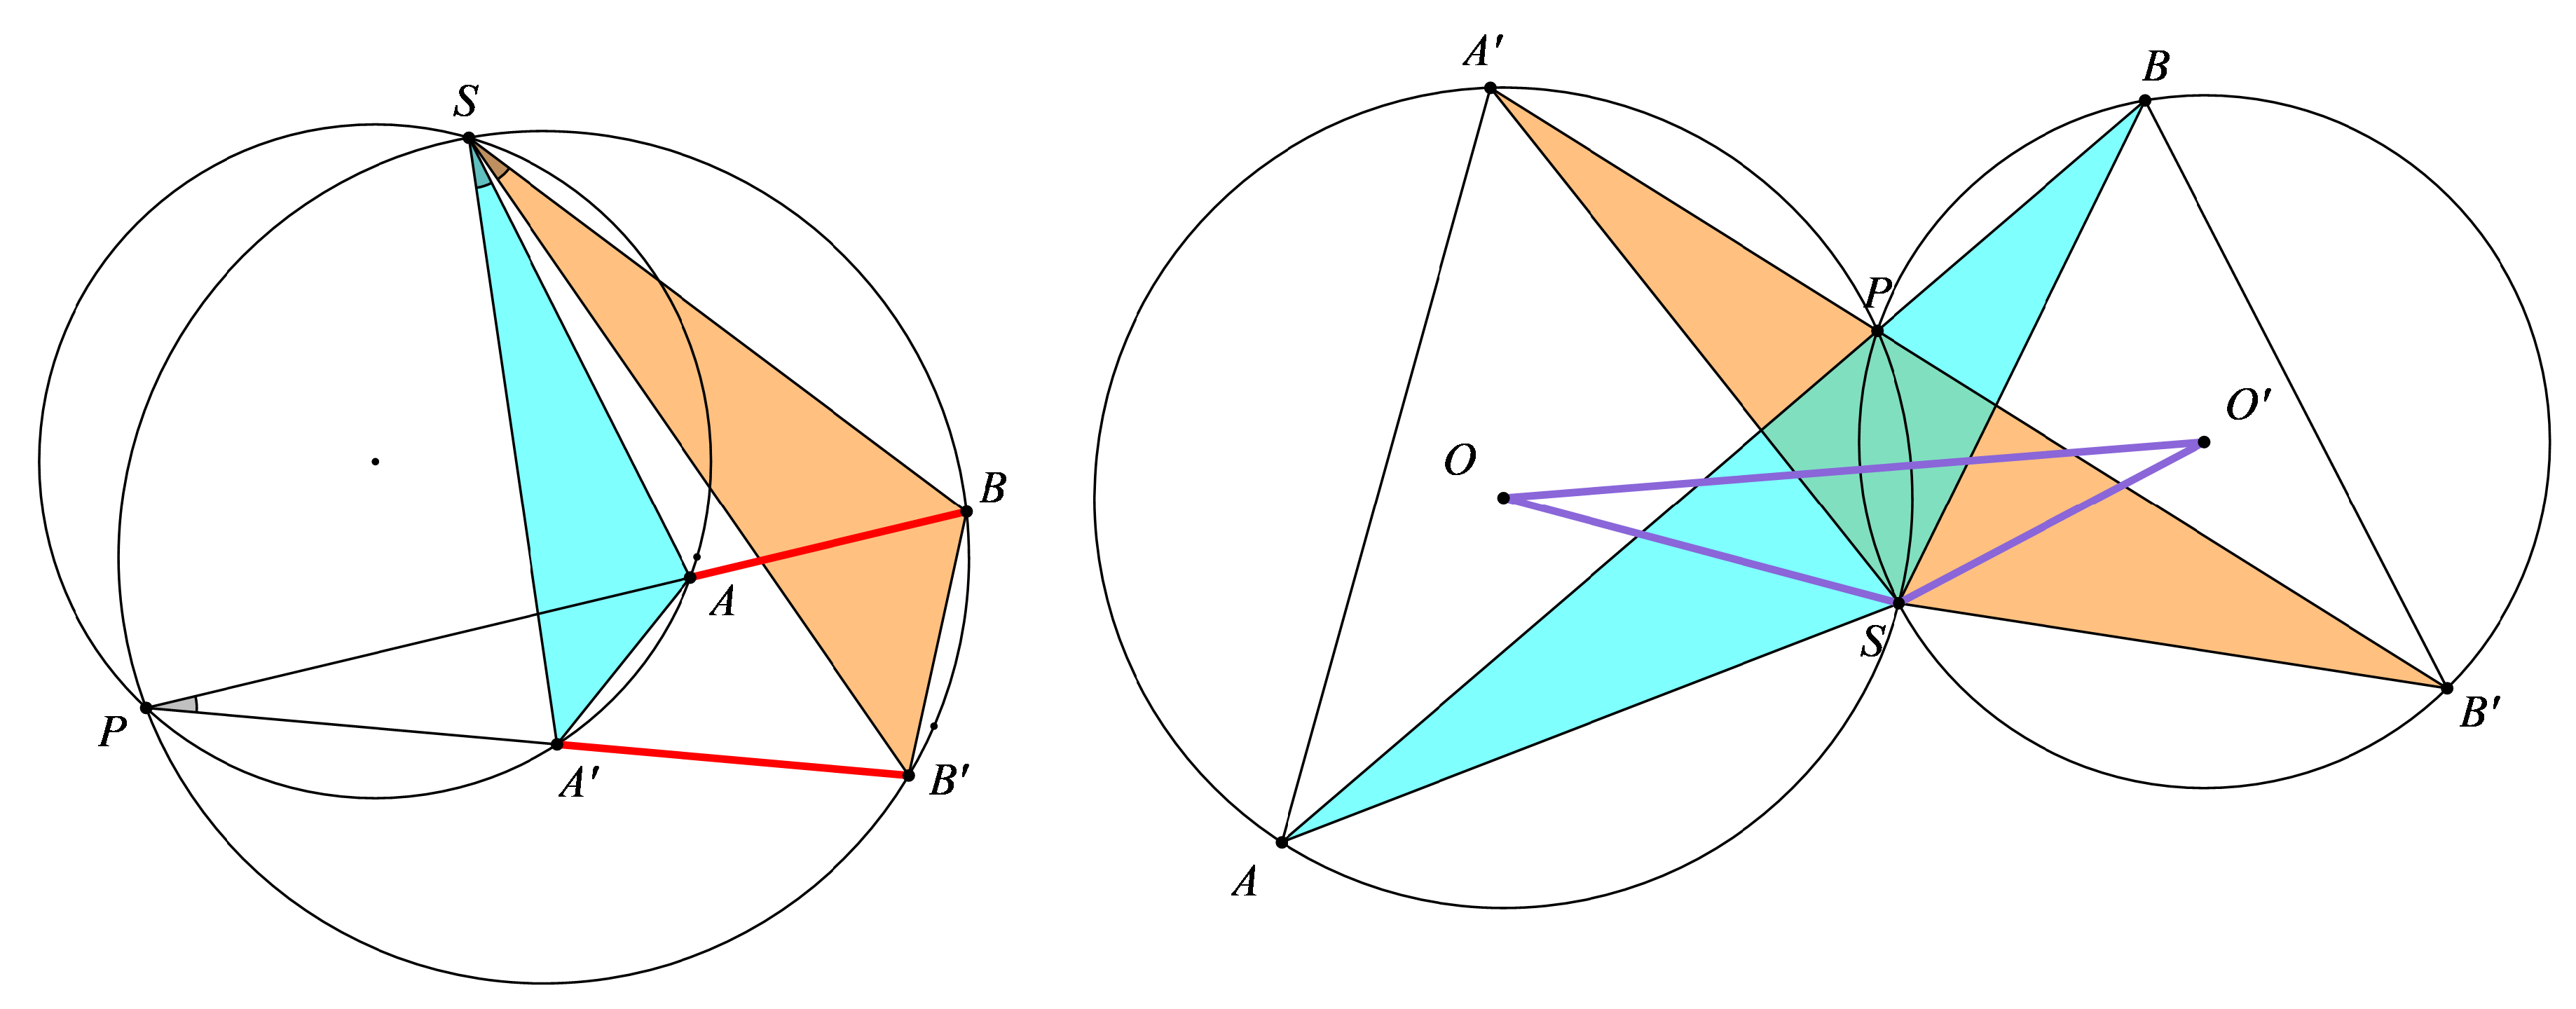
\includegraphics[width=1\linewidth]{2}
		\vspace*{-20pt}
	\end{figure}
	\textit{Chứng minh.} Gọi $S$ là giao điểm thứ hai của các đường tròn $(PAA')$ và $(PBB')$. Ta có $(AS,AP)=(A'S,A'P) (\,\,\bmod \,\,\, \pi)$, $(BS,BP)=(B'S,B'P)(\bmod  \pi)$ nên hai tam giác $SAB$ và $SA'B'$ đồng dạng. Như vậy, $S$ là tâm của phép vị tự quay biến đoạn $AB$ thành đoạn $A'B'$. 
	\vskip 0.1cm
	\textbf{\color{hoccungpi}Nhận xét.}  Ta có một số quan sát sau:
	\vskip 0.1cm
	$1)$ Nếu $S$ là tâm phép vị tự quay biến đoạn $AB$ thành đoạn $A'B'$ thì dễ thấy hai tam giác $SAB$ và $SA'B'$ đồng dạng nên $S$ cũng là tâm của phép vị tự quay biến đoạn $AA'$ thành đoạn $BB'$.
	\vskip 0.1cm 
	$2)$ Nếu hai đường tròn $(PAA')$, $(PBB')$  có tâm lần lượt là $O$, $O'$ thì $S$ cũng là tâm của phép vị tự quay biến đường tròn $(O)$ thành đường tròn $(O')$. Do đó ta có các tam giác $SAB,SA'B'$ và $SOO'$ đồng dạng.
	\vskip 0.1cm
	$3)$ Nếu $AA'$ cắt $BB'$ tại $Q$ thì các điểm $Q,S,A,B$ đồng viên và các điểm $Q,S,A',B'$ đồng viên. Điểm $S$ chính là điểm Miquel của tứ giác toàn phần xác định bởi $ABB'A'$.
	\begin{figure}[H]
		\vspace*{-5pt}
		\centering
		\captionsetup{labelformat= empty, justification=centering}
		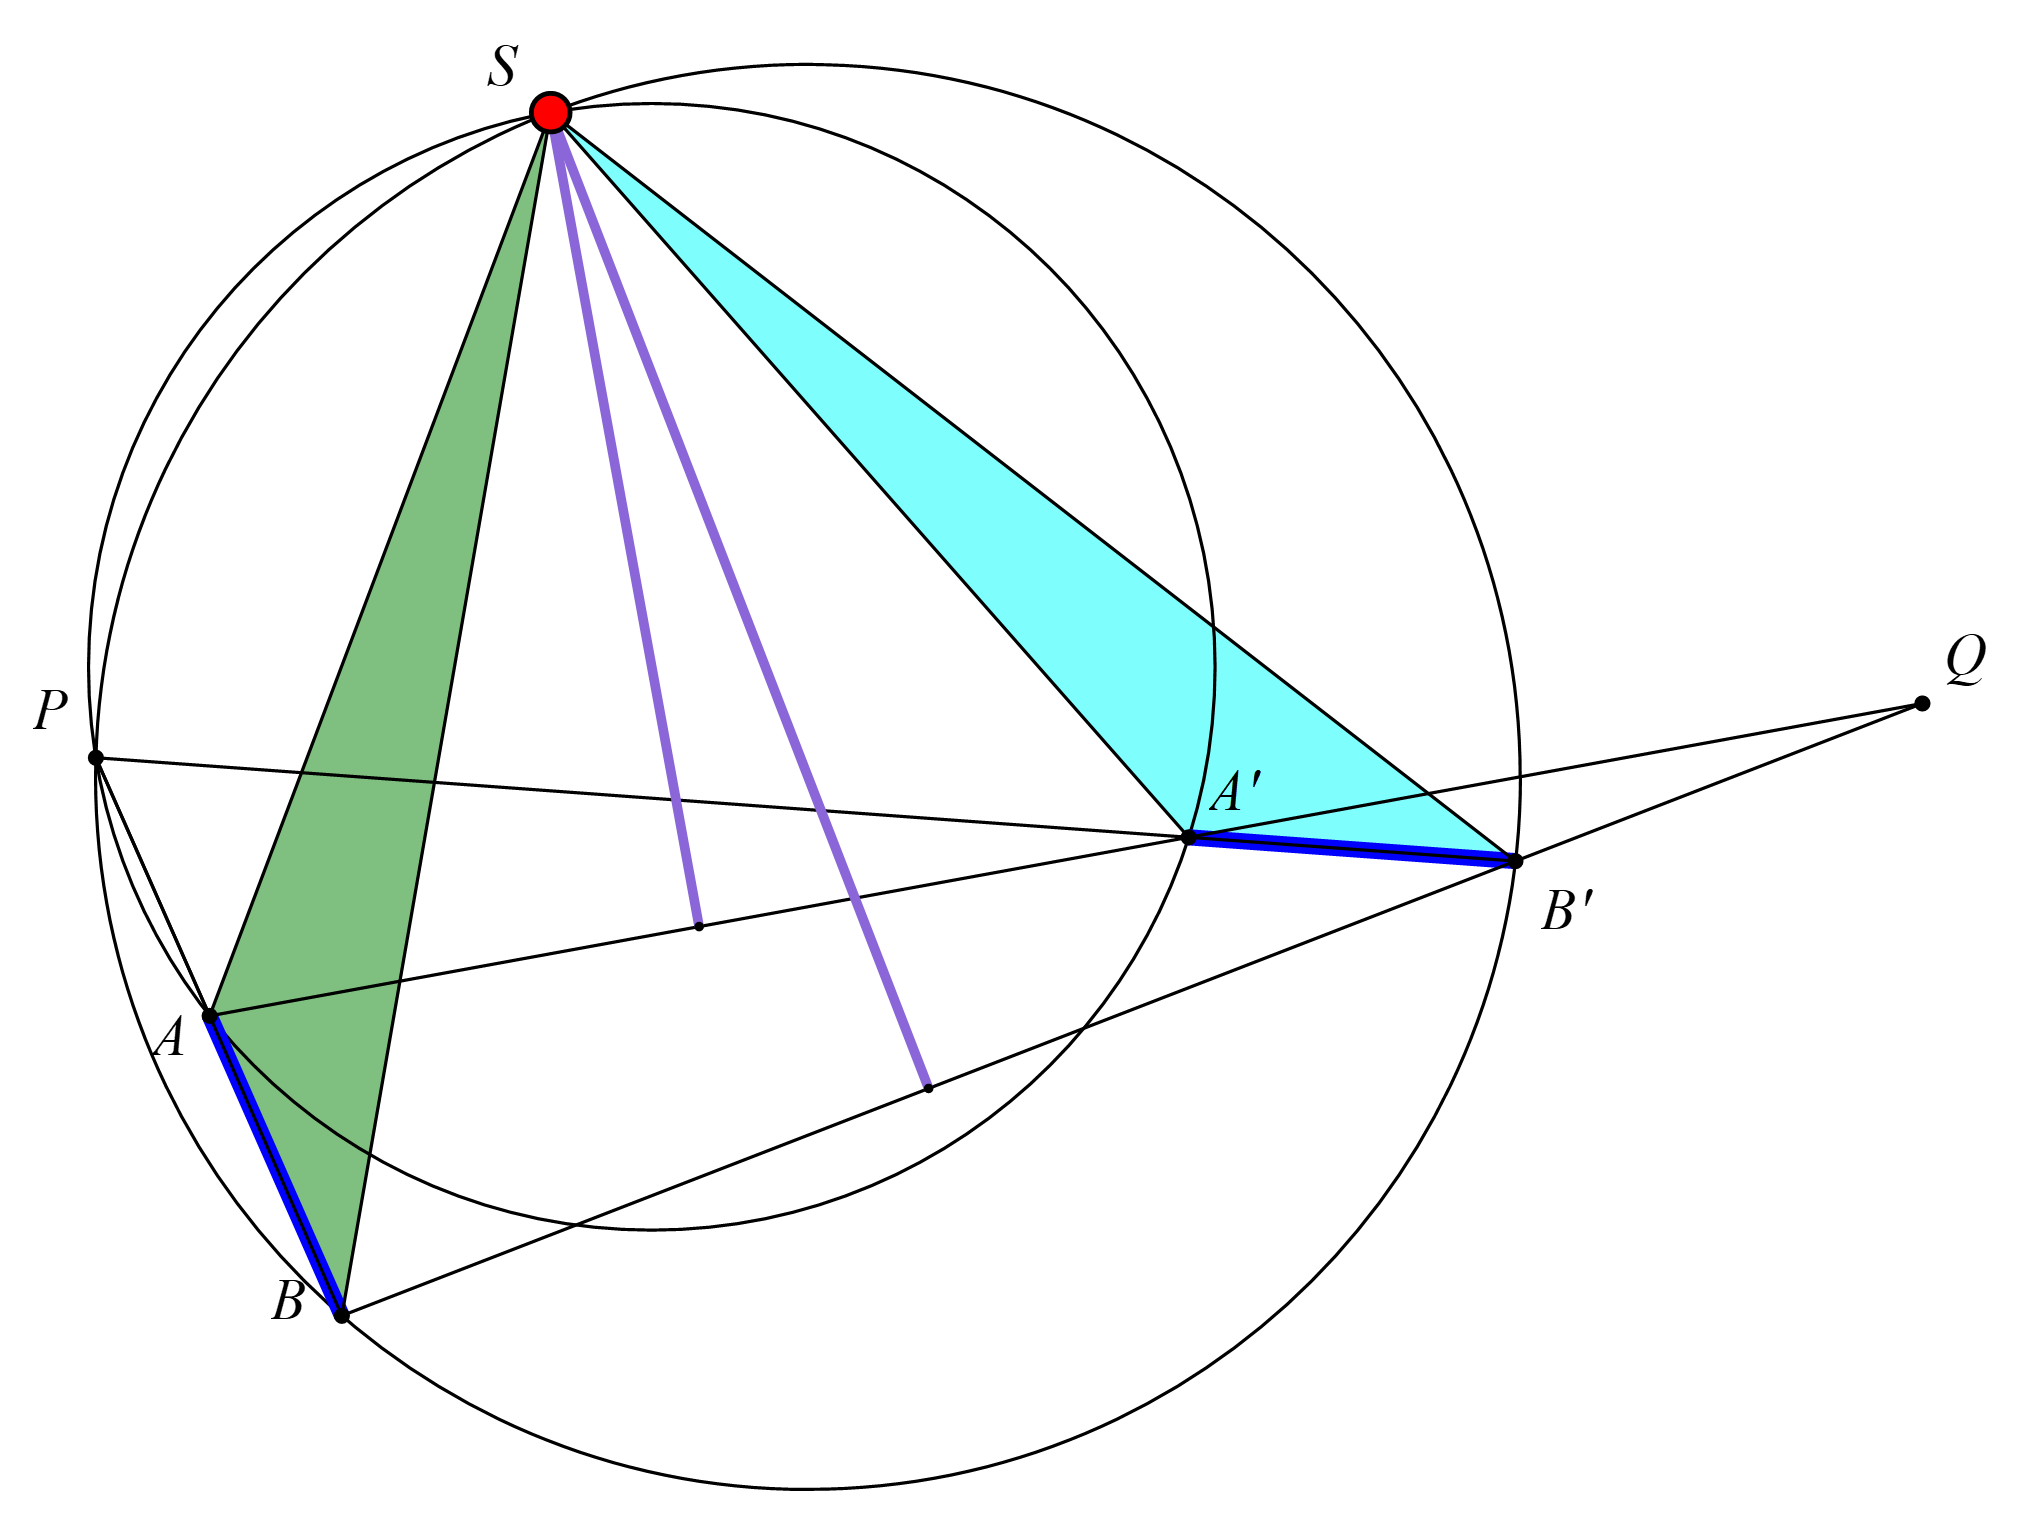
\includegraphics[scale=0.75]{3}
		\vspace*{-10pt}
	\end{figure}
	$4)$ Với hai đoạn thẳng $AB,A'B'$ không cùng phương, luôn có hai phép vị tự quay biến đoạn thẳng này thành đoạn thẳng kia.
	\vskip 0.1cm
	$5)$ Trong trường hợp đặc biệt khi $AB=A'B'$, ta thu lại được kết quả của Bổ đề $1$ ở trên.
	\vskip 0.1cm
	\textbf{\color{hoccungpi}$\pmb{2.}$  Một số áp dụng}
	\vskip 0.1cm
	Bổ đề $1$ và $2$ tỏ ra khá hữu ích trong một số tình huống. Trong bài viết này, chúng tôi xin giới thiệu ứng dụng của chúng trong việc chứng minh các đoạn thẳng bằng nhau, chỉ ra một đường thẳng hoặc đường tròn đi qua điểm cố định và chứng minh một số đường tròn đồng quy.
	\vskip 0.1cm
	$\pmb{2.1.}$ \textbf{\color{hoccungpi}Chứng minh hai đoạn thẳng bằng nhau}
	\vskip 0.1cm
	Ví dụ đầu tiên được lấy từ một bài toán Vô địch Liên bang Nga năm $2006$.
	\vskip 0.1cm
	\textbf{\color{hoccungpi}Ví dụ $\pmb{1.}$} Cho tam giác $ABC$ nội tiếp đường tròn $(O)$. Hai điểm $M,N$ thay đổi trên $AB,AC$ sao cho $MN \parallel BC$, $MN$ cắt $(O)$ tại  $P,Q$ ($M$ nằm giữa $P$ và $N$). Gọi $J,K$ tương ứng là tâm đường tròn nội tiếp các tam giác $APB$, $AQC$ và $T$ là trung điểm của cung $BC$ chứa $A$ của đường tròn $(O)$. Chứng minh rằng $TJ=TK$.
	\begin{figure}[H]
		\vspace*{-5pt}
		\centering
		\captionsetup{labelformat= empty, justification=centering}
		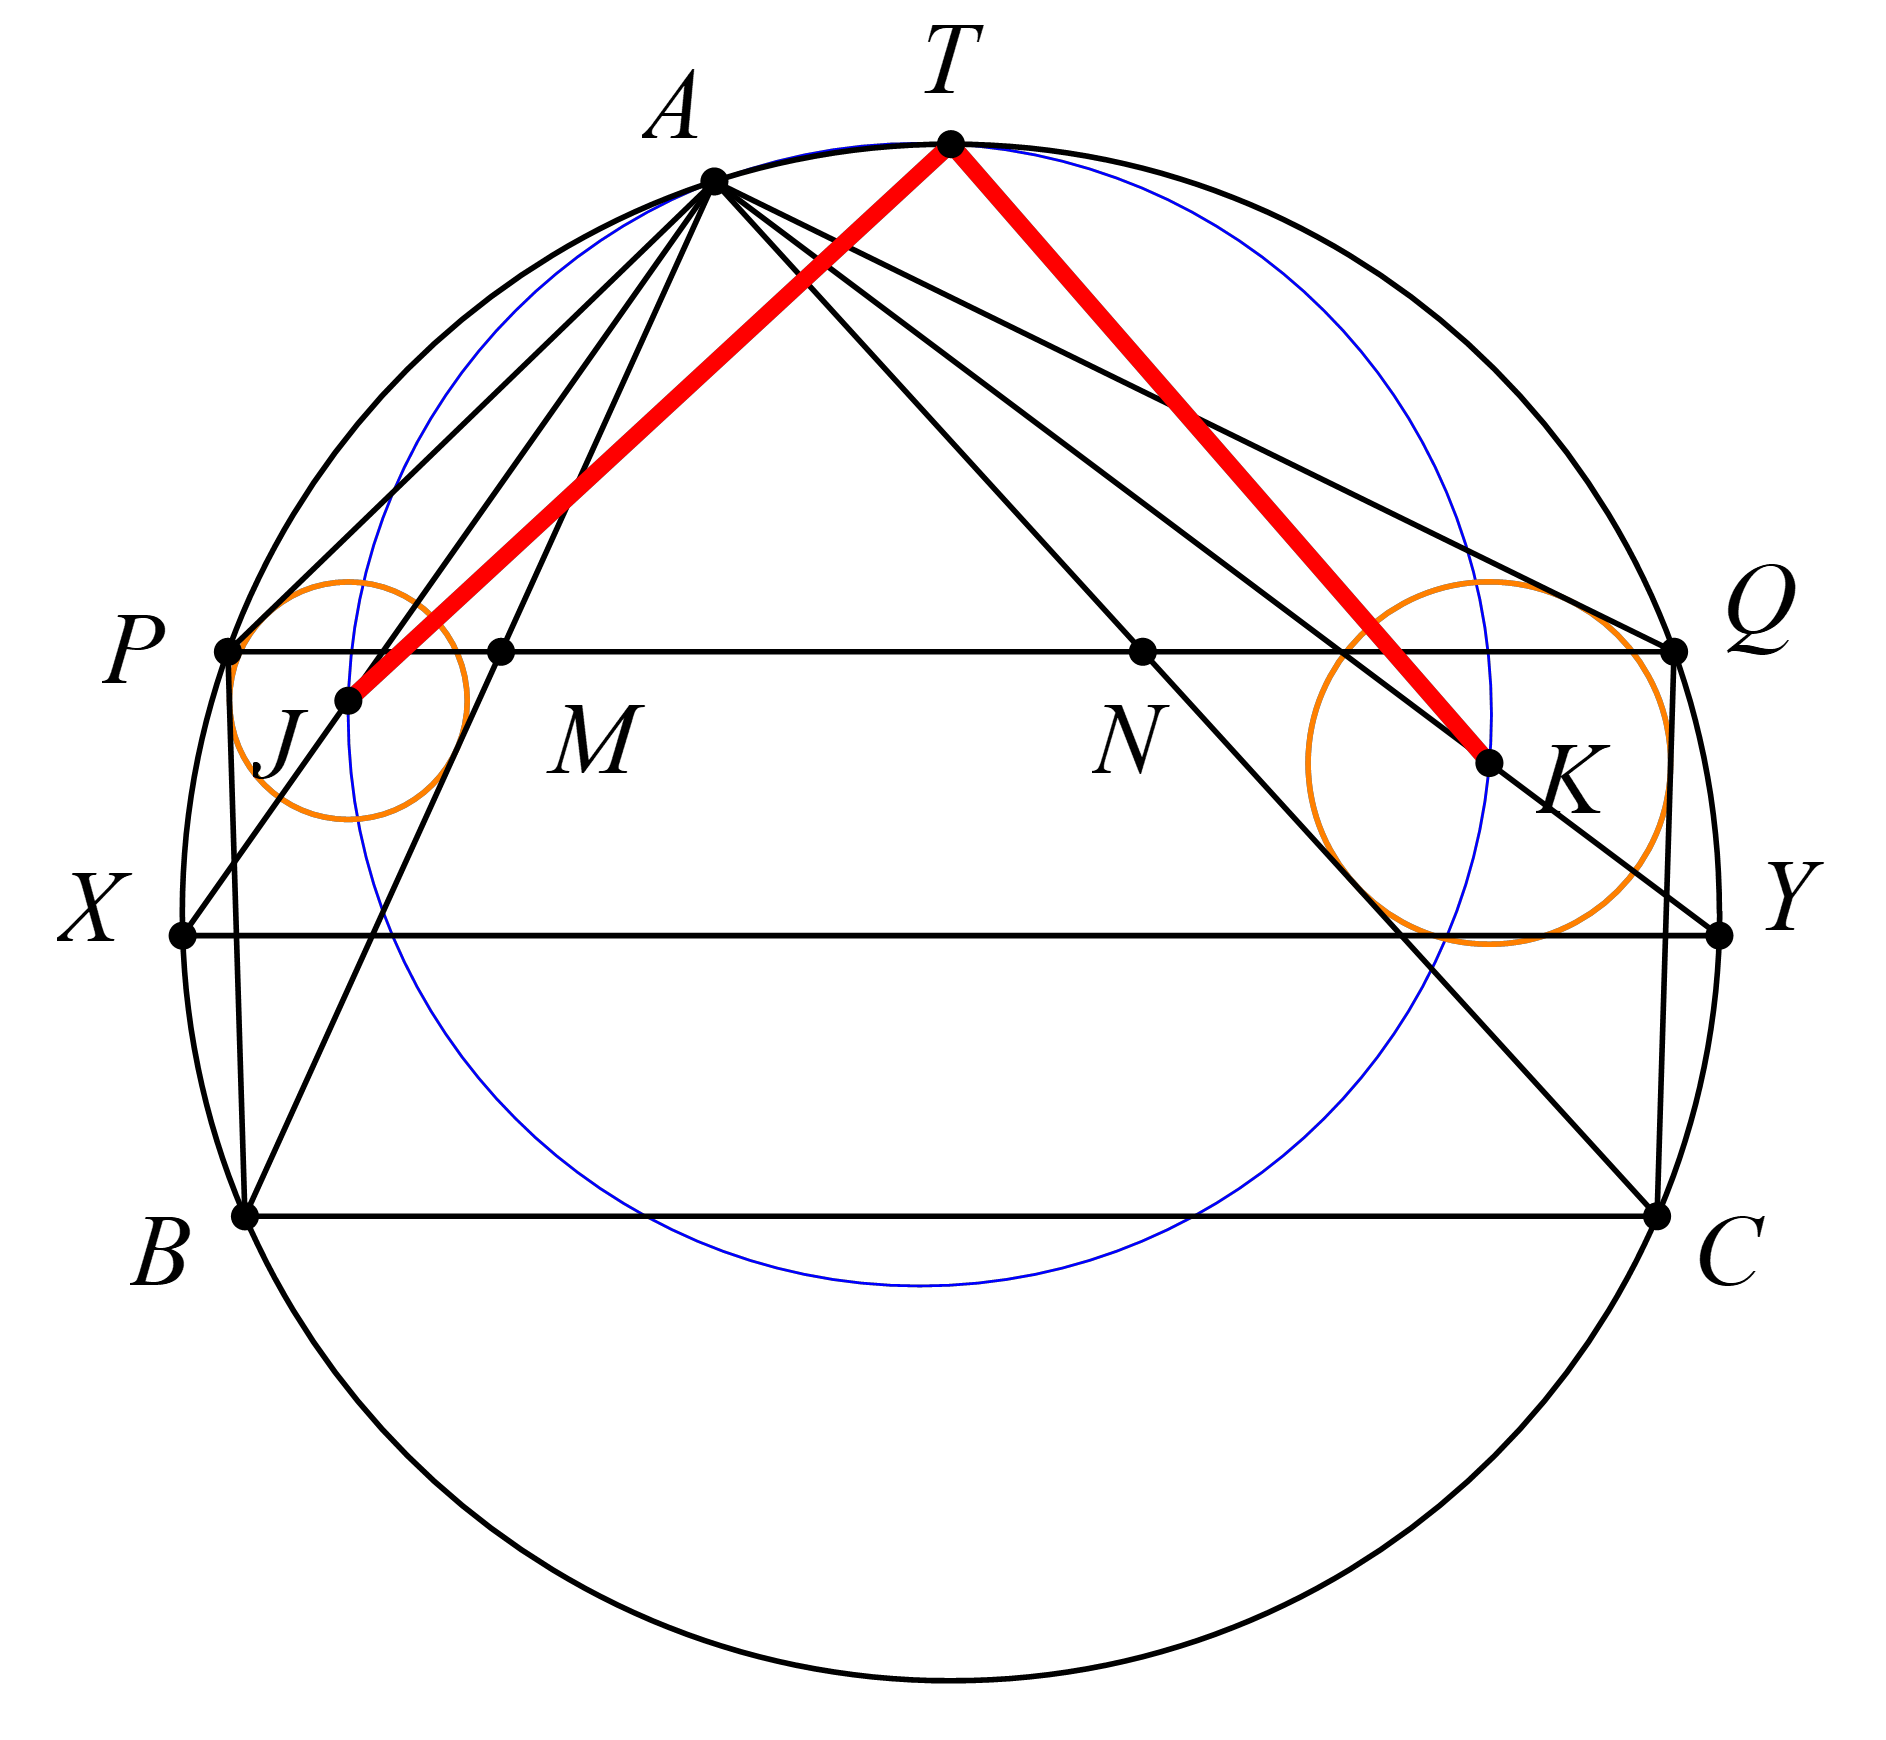
\includegraphics[width= 0.9\linewidth]{4}
		\vspace*{-10pt}
	\end{figure}
	\textit{Phân tích:} Đề bài xuất hiện mô hình trung điểm cung $T$ và yêu cầu chứng minh $TJ=TK$. Đây là dấu hiệu khá rõ để ta vận dụng kết quả của Bổ đề $1$. Ta cần tìm ra hai đoạn thẳng bằng nhau có các đầu mút là $J$, $K$. Để ý tới giả thiết $MN$ song song với $BC$ và tính chất của tâm đường tròn nội tiếp là ta có thể tiếp cận được bài toán.
	\vskip 0.1cm
	\textit{Lời giải.} Giả sử $AJ,AK$ cắt $(ABC)$ tương ứng tại $X$, $Y$. Dễ thấy $X$, $Y$ tương ứng là trung điểm của các cung $PB$, $QC$ của đường tròn $(ABC)$. Theo một kết quả quen thuộc thì $XB=XP=XJ$ và  $YC=YQ=YK$. Mà $YC=XB$ nên $KY=XJ$. Áp dụng Bổ đề $1$ cho tam giác $AXY$, với hai điểm $J,K$ thỏa $XJ=YK$, ta suy ra đường trung trực của đoạn thẳng $JK$ đi qua trung điểm $T$ của cung $BC$ chứa $A$ của đường tròn $(ABC)$. Vậy $TJ=TK$.
	\vskip 0.1cm
	Ví dụ sau đây, được lấy từ kỳ thi Vô địch Liên bang Nga năm $2014$, cũng có thể được giải quyết bằng cách tương tự.
	\vskip 0.1cm
	\textbf{\color{hoccungpi}Ví dụ $\pmb{2.}$} Cho tam giác $ABC$ có $AB > AC$. Các điểm $M,N$ tương ứng nằm trên các cạnh $AC,AB$ sao cho $BN=CM$. Đường thẳng $MN$ cắt $BC$ tại $P$. Gọi $I$ là tâm đường tròn nội tiếp tam giác $PNB$, $J$ là tâm đường tròn bàng tiếp góc $P$ của tam giác $PMC$ và $T$ là trung điểm cung $BC$ chứa $A$. Chứng minh rằng  $TI=TJ$.
	\vskip 0.1cm
	\textit{Phân tích:} Đề bài tiếp tục xuất hiện mô hình trung điểm cung $T$ và hai đoạn thẳng $BN,CM$ bằng nhau nên cũng gợi ý đến việc vận dụng Bổ đề $1$. Tuy nhiên ý tưởng chứng minh $TI=TJ$ không giống như lời giải của ví dụ ở trên mà phải dùng đến một phép quay phù hợp. với tâm là trung điểm $T$ của cung $BC$ chứa $A$.
	\begin{figure}[H]
		\vspace*{-5pt}
		\centering
		\captionsetup{labelformat= empty, justification=centering}
		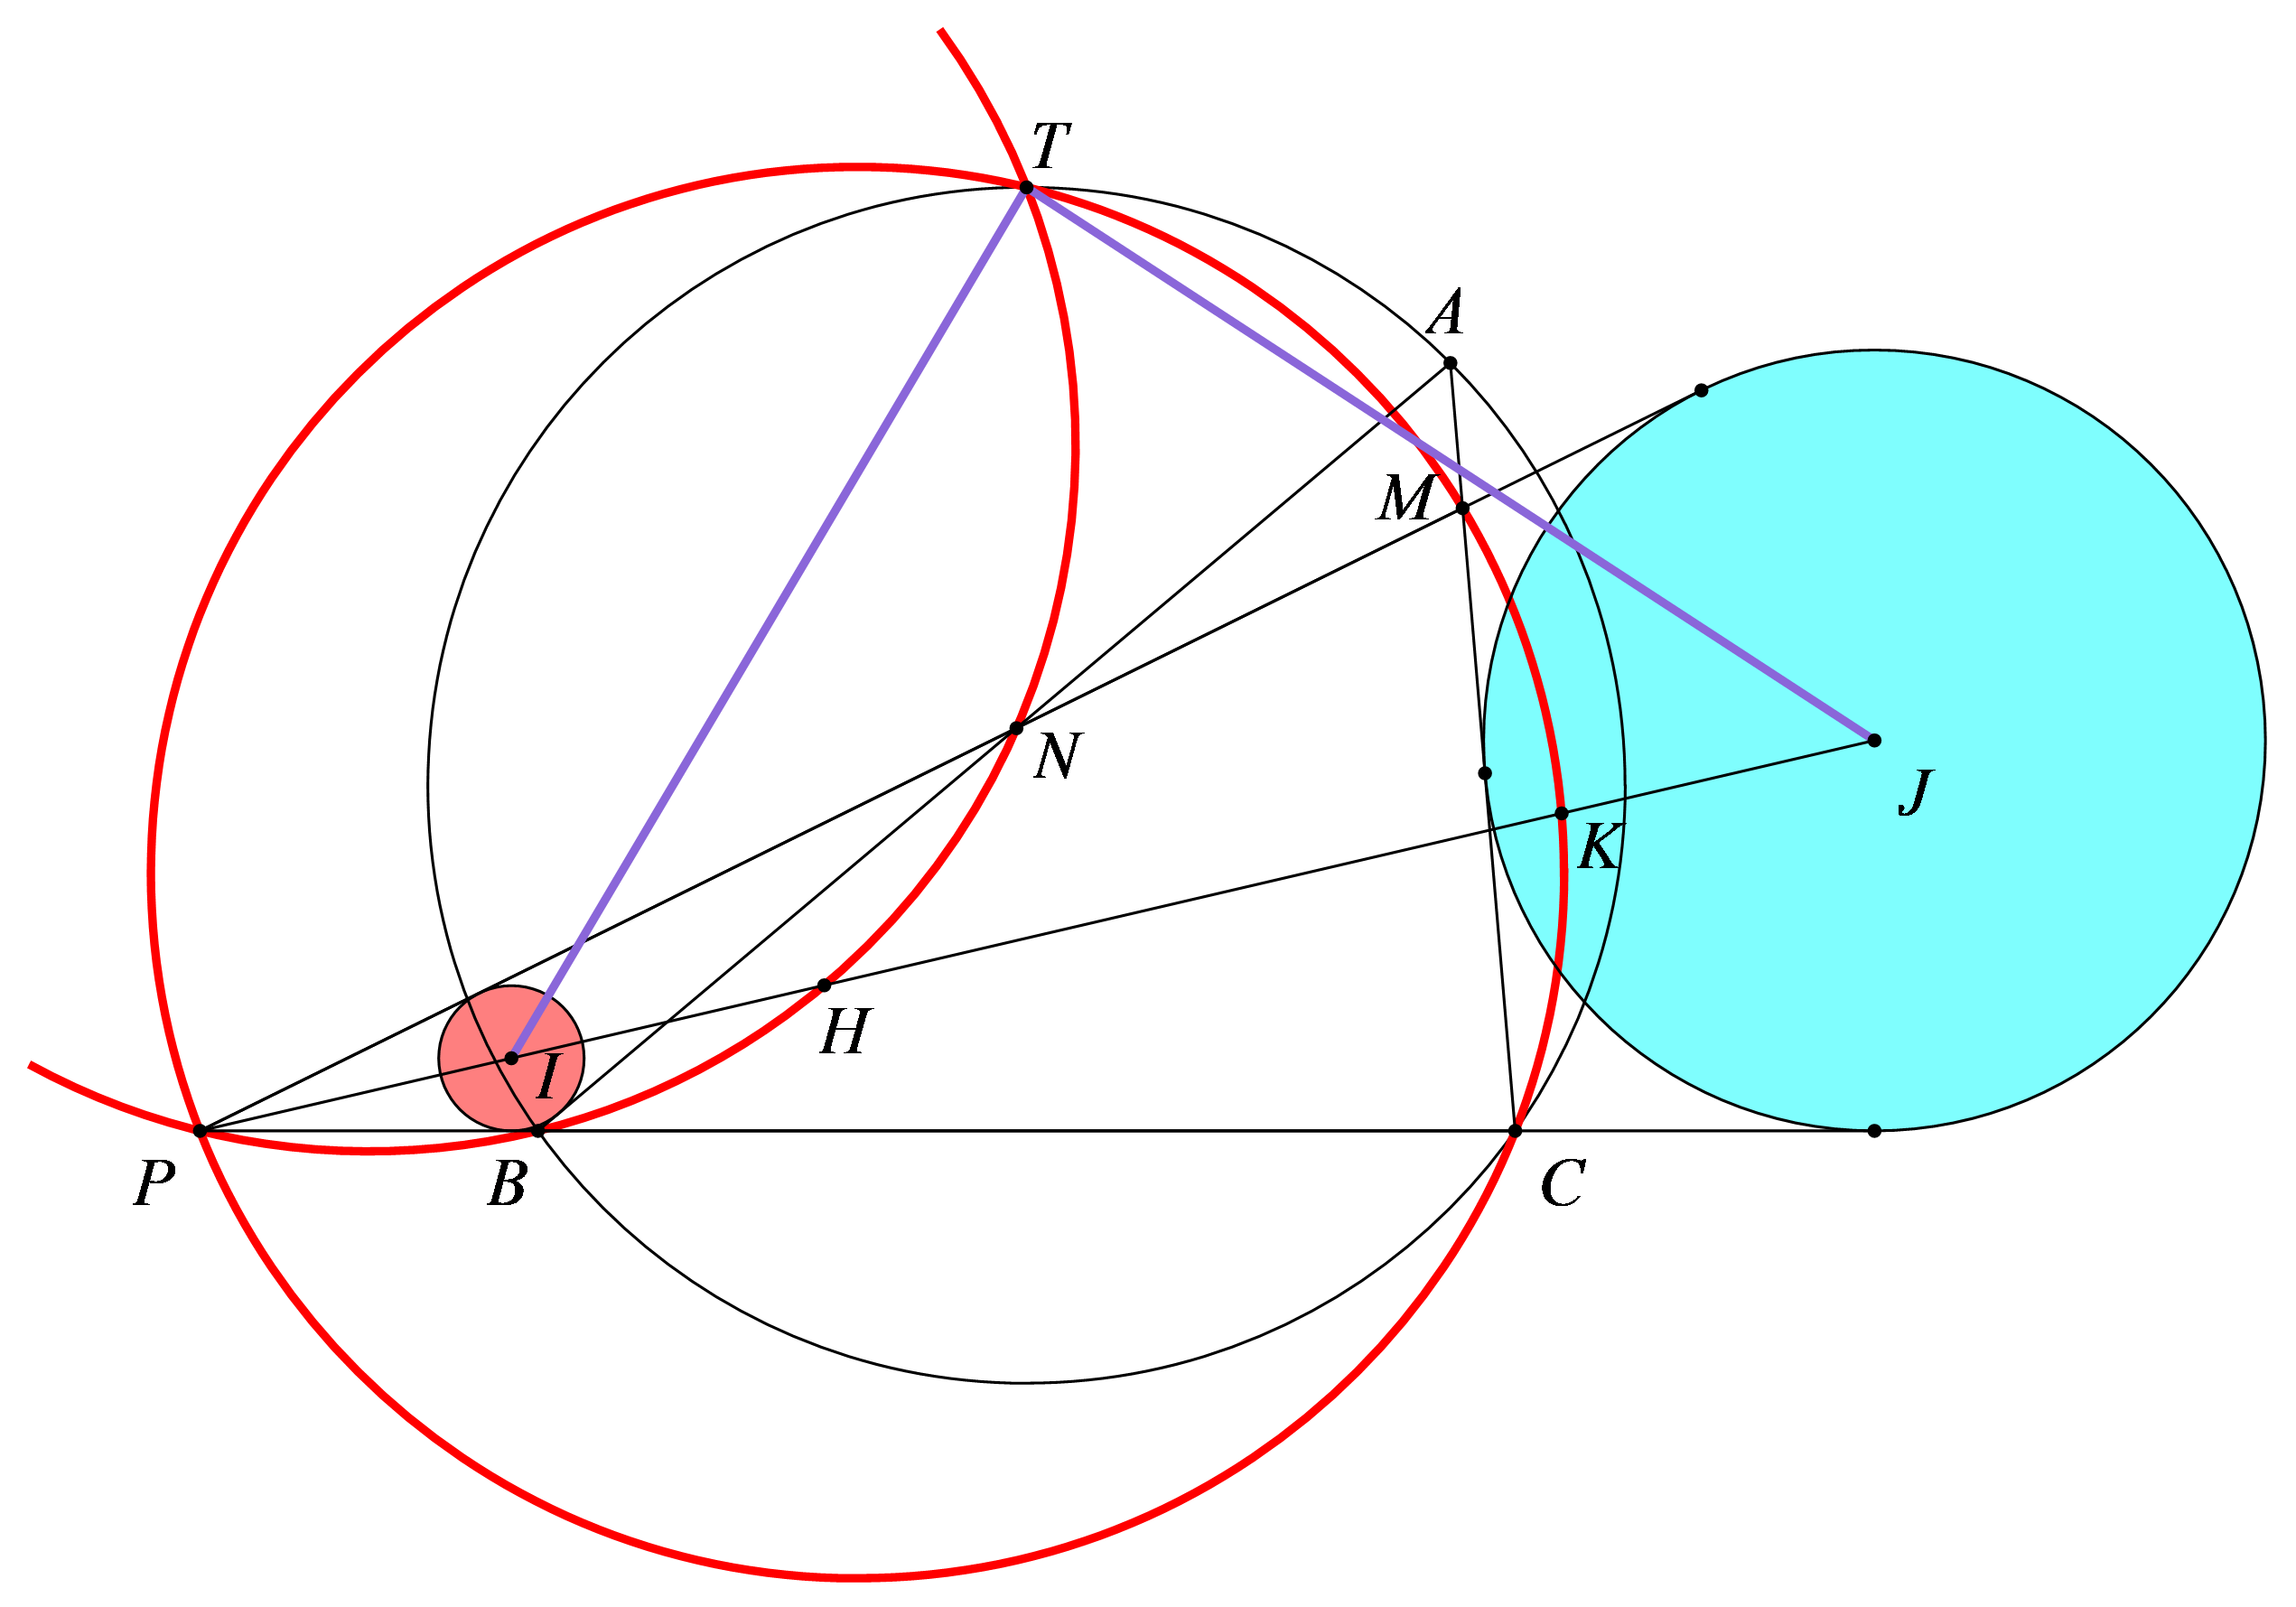
\includegraphics[width= 1\linewidth]{5}
		\vspace*{-10pt}
	\end{figure}
	\textit{Lời giải.} Theo Bổ đề $1$ thì tồn tại phép quay tâm $T$ biến $B,\,N$ lần lượt thành $C,\,M$, do đó tam giác $TNB$ biến thành tam giác $TMC$, đường tròn $(TNB)$ biến thành đường tròn $(TMC)$ suy ra $H$ biến thành $K$ ($H, K$ lần lượt là trung điểm cung $BN,CM$). Dễ chứng minh được $HB=HN=HI$; $KC=KM=KJ$. Mà $BN=CM$ nên ta có $HI=KJ$, từ đó suy ra được $TI=TJ$.
	\vskip 0.1cm
	\textbf{\color{hoccungpi}Ví dụ $\pmb{3.}$} Cho tứ giác lồi $ABCD$ có hai đường chéo $AC$ và $BD$ cắt nhau tại $P$. Gọi $I,J$ lần lượt là tâm các đường tròn $(PAD)$, $(PBC)$. Gọi $M,N,O$ lần lượt là trung điểm các đoạn thẳng $AC,BD,IJ$. Chứng minh $OM=ON$.
	\begin{figure}[H]
		\vspace*{-5pt}
		\centering
		\captionsetup{labelformat= empty, justification=centering}
		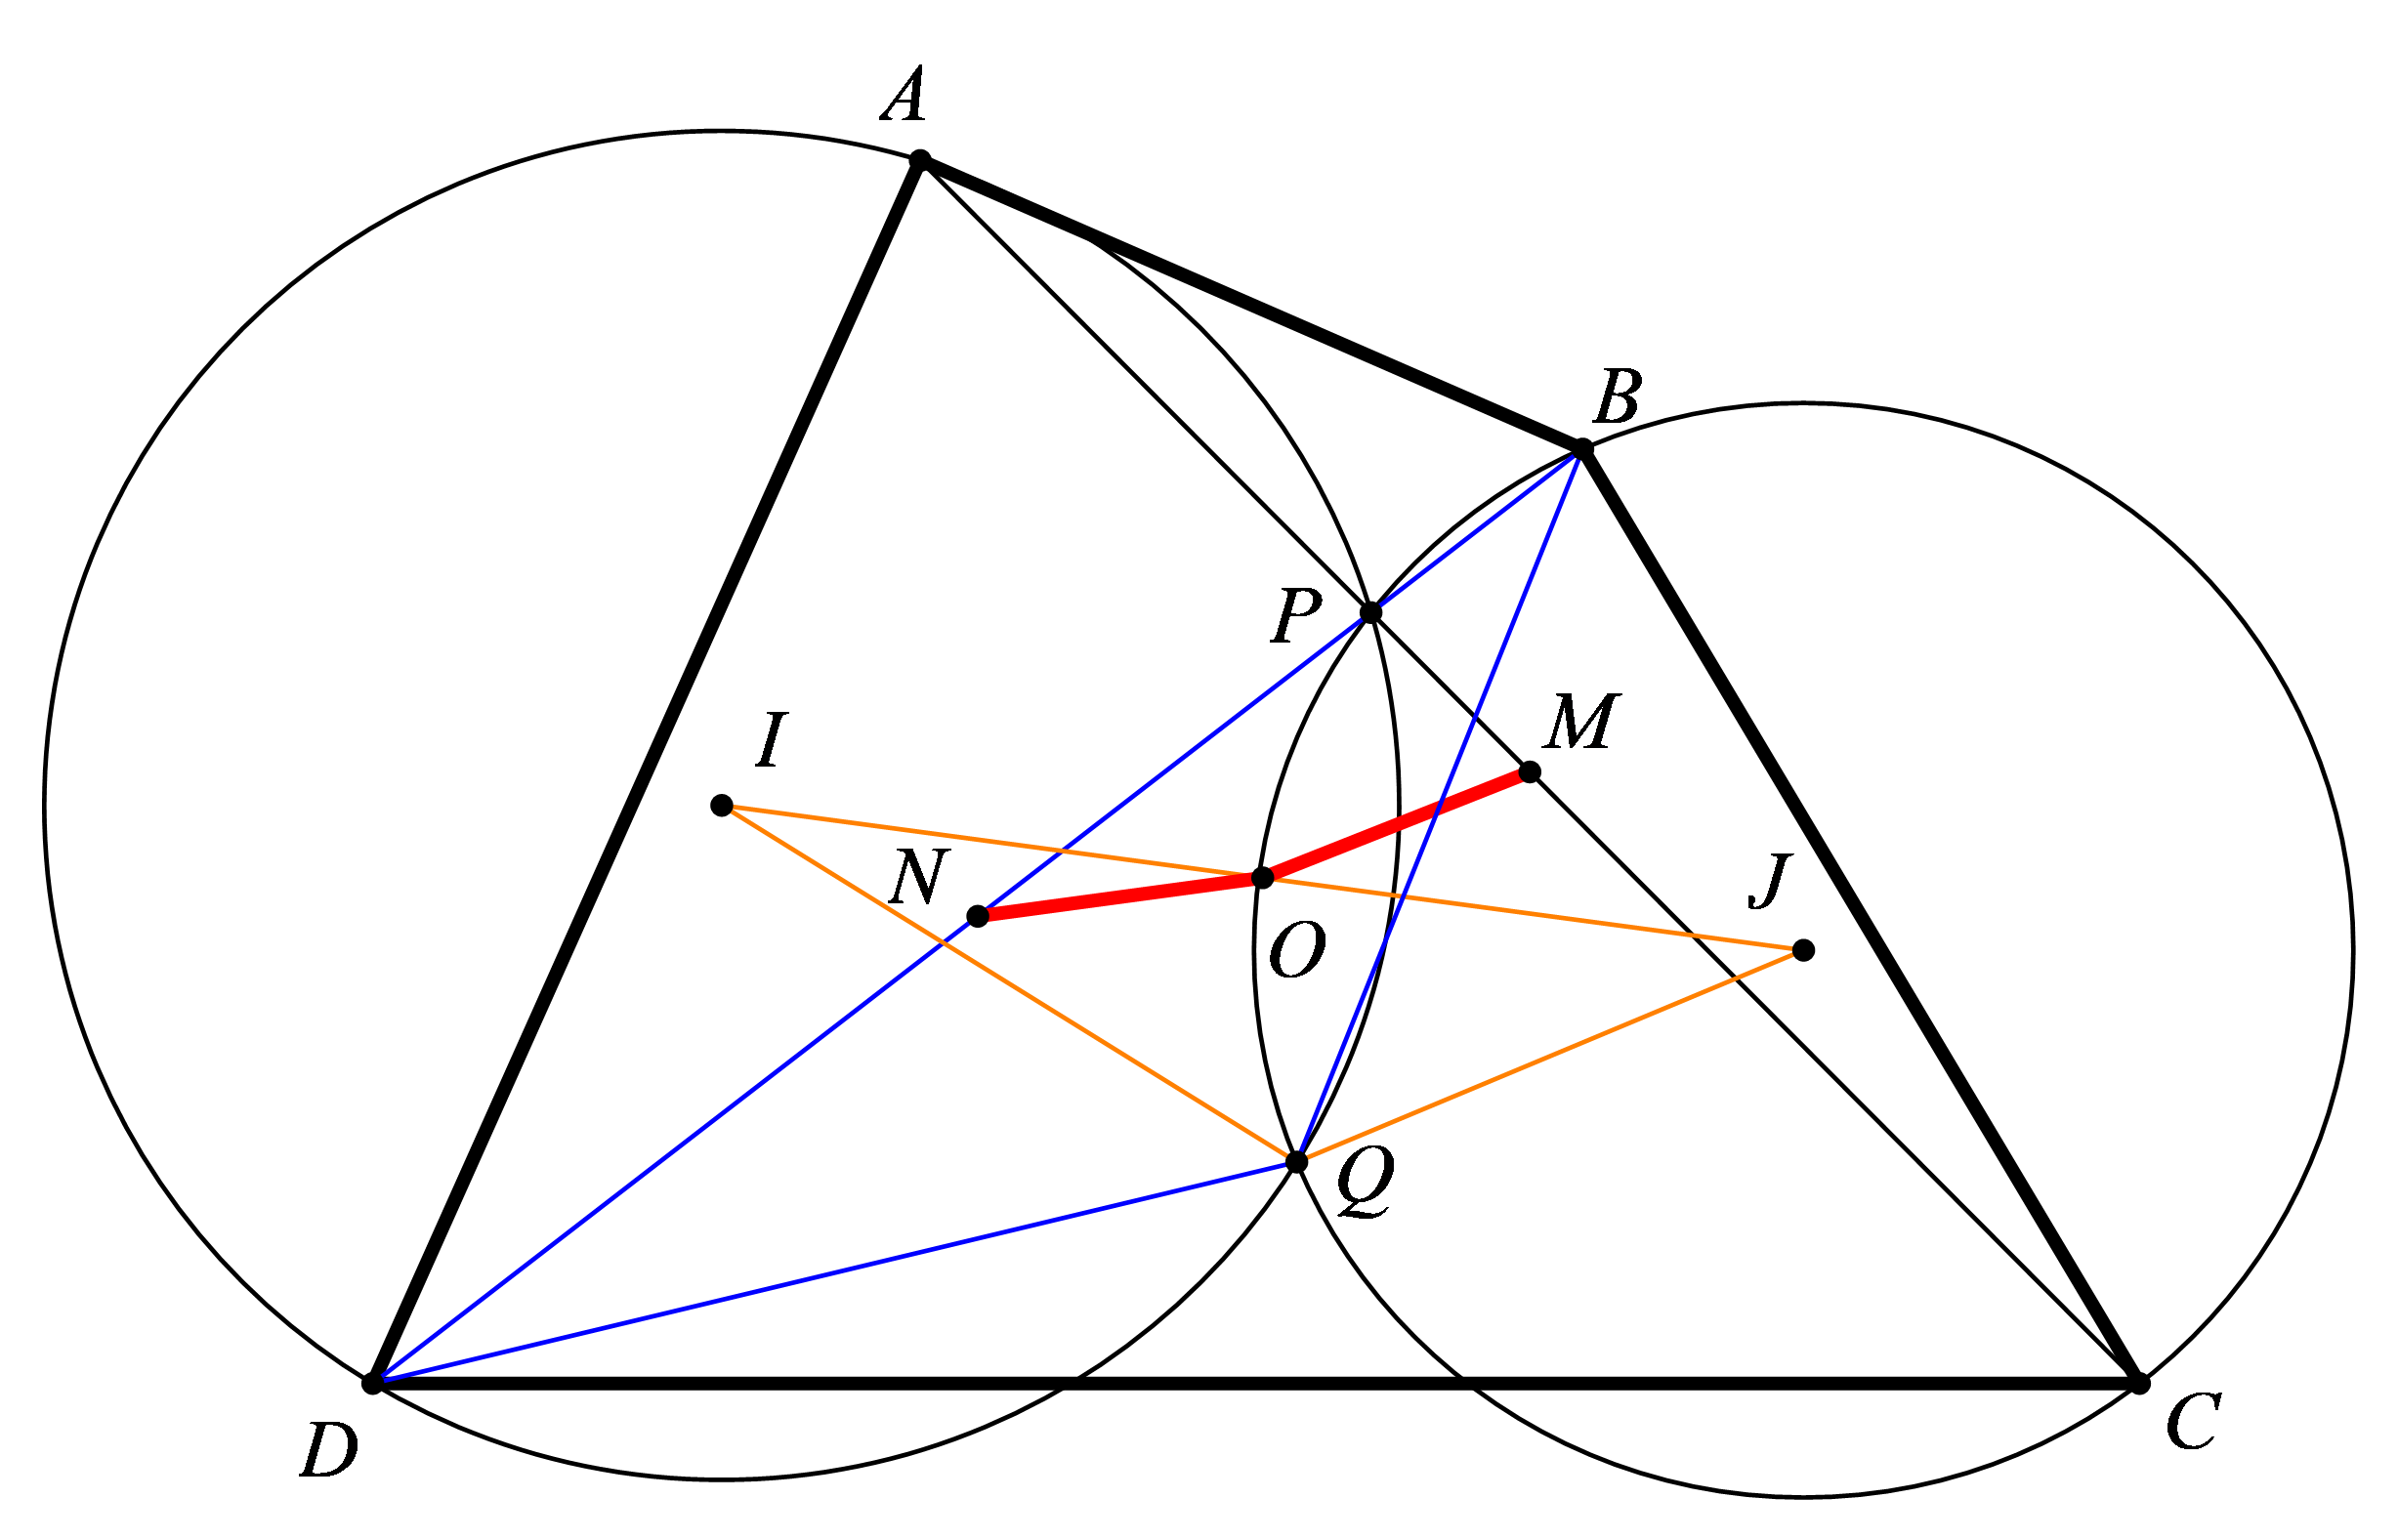
\includegraphics[width= 1\linewidth]{6}
		\vspace*{-15pt}
	\end{figure}
	\textit{Phân tích.} Bài toán xuất hiện mô hình hai đoạn thẳng cắt nhau: $AC$ và $BD$ cắt nhau tại $P$; ngoài ra, hai đường tròn $(PAD)$ và $(PBC)$ cắt nhau tại điểm thứ hai là $Q$ nên chúng là các dấu hiệu để áp dụng Bổ đề $2$ trong việc tiếp cận bài toán. Điểm $Q$ chính là tâm của phép vị tự quay mà ta quan tâm.
	\begin{figure}[H]
		\vspace*{-10pt}
		\centering
		\captionsetup{labelformat= empty, justification=centering}
		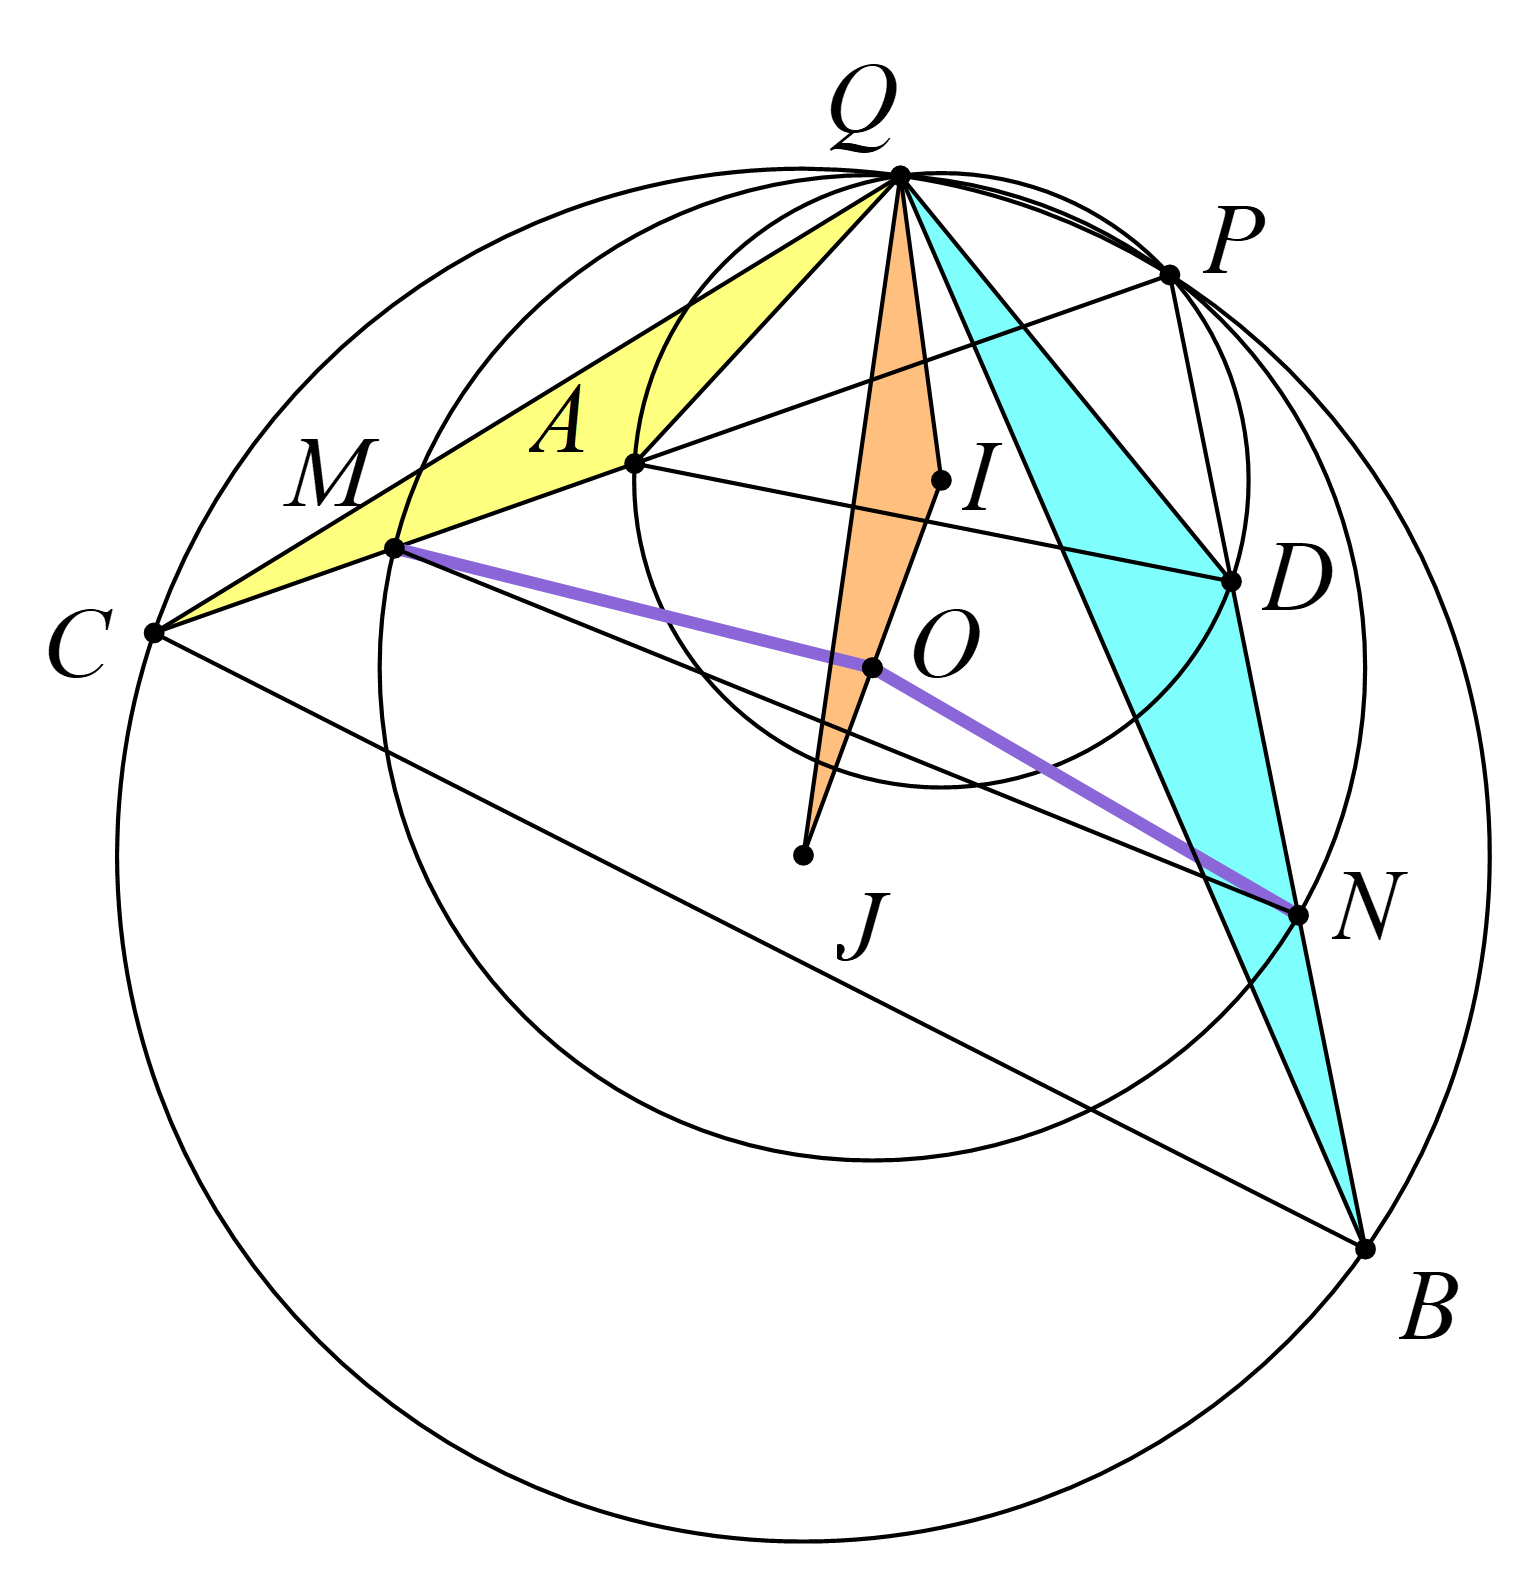
\includegraphics[width= 0.9\linewidth]{7}
		\vspace*{-10pt}
	\end{figure}
	\textit{Lời giải.} Áp dụng Bổ đề $2$ cho hai đoạn thẳng $AC$ và $BD$, do chúng cắt nhau tại $P$, ta biết rằng tồn tại phép vị tự quay $f$ với tâm $Q$ là giao điểm thứ hai (khác $P$) của các đường tròn $(PAD)$ và $(PBC)$. Phép vị tự quay $f$ biến $A$ thành $C$, biến $D$ thành $B$. Ngoài ra, ta biết rằng cũng tồn tại phép vị tự quay $g$ với tâm là $Q$ biến $A$ thành $D$, biến $C$ thành $B$; do đó đoạn $AC$  biến thành đoạn $DB$, dẫn đến $g$ biến $M$ thành $N$. Như vậy, các đường tròn $(PAD)$, $(PBC)$, $(PMN)$ cùng đi qua $Q$. Vì $f$ biến $A$ thành $C,D$ thành $B$ và $I$ thành $J$ nên các tam giác $QDB,QAC,QIJ$ đồng dạng với nhau. Từ đó suy ra các tam giác $QDN,QAM$ và $QIO$ đồng dạng. Do đó tồn tại một phép vị tự quay tâm $Q$ biến $D$ thành $N$, $A$ thành $M$ và $I$ thành $O$. Khi đó $O$ chính là tâm đường tròn $(QMN)$ nên ta có $OM=ON$.
	\vskip 0.1cm
	\textit{Nhận xét.} Kết luận của bài toán vẫn còn đúng khi $A,B,C,D$ là bốn điểm bất kỳ sao cho $AC$ và $BD$ cắt nhau. 
	\vskip 0.1cm
	$\pmb{2.2.}$ \textbf{\color{hoccungpi}Chứng minh tính thẳng hàng, đồng quy}
	\vskip 0.1cm
	Bài toán sau đây, được lấy từ các bài toán đề nghị thi Toán quốc tế năm $2006$, minh họa một ứng dụng khác của các Bổ đề $1$ và $2$.
	\vskip 0.1cm
	\textbf{\color{hoccungpi}Ví dụ $\pmb{4.}$} Cho ngũ giác lồi $ABCDE$ thỏa mãn $\angle BAC = \angle CAD = \angle DAE,$ $\angle CBA = \angle DCA =\angle EDA$. Gọi $P$ là giao điểm của $BD$ và $CE$. Chứng minh rằng $AP$ đi qua trung điểm của $CD$. 
	\begin{figure}[H]
		\vspace*{-5pt}
		\centering
		\captionsetup{labelformat= empty, justification=centering}
		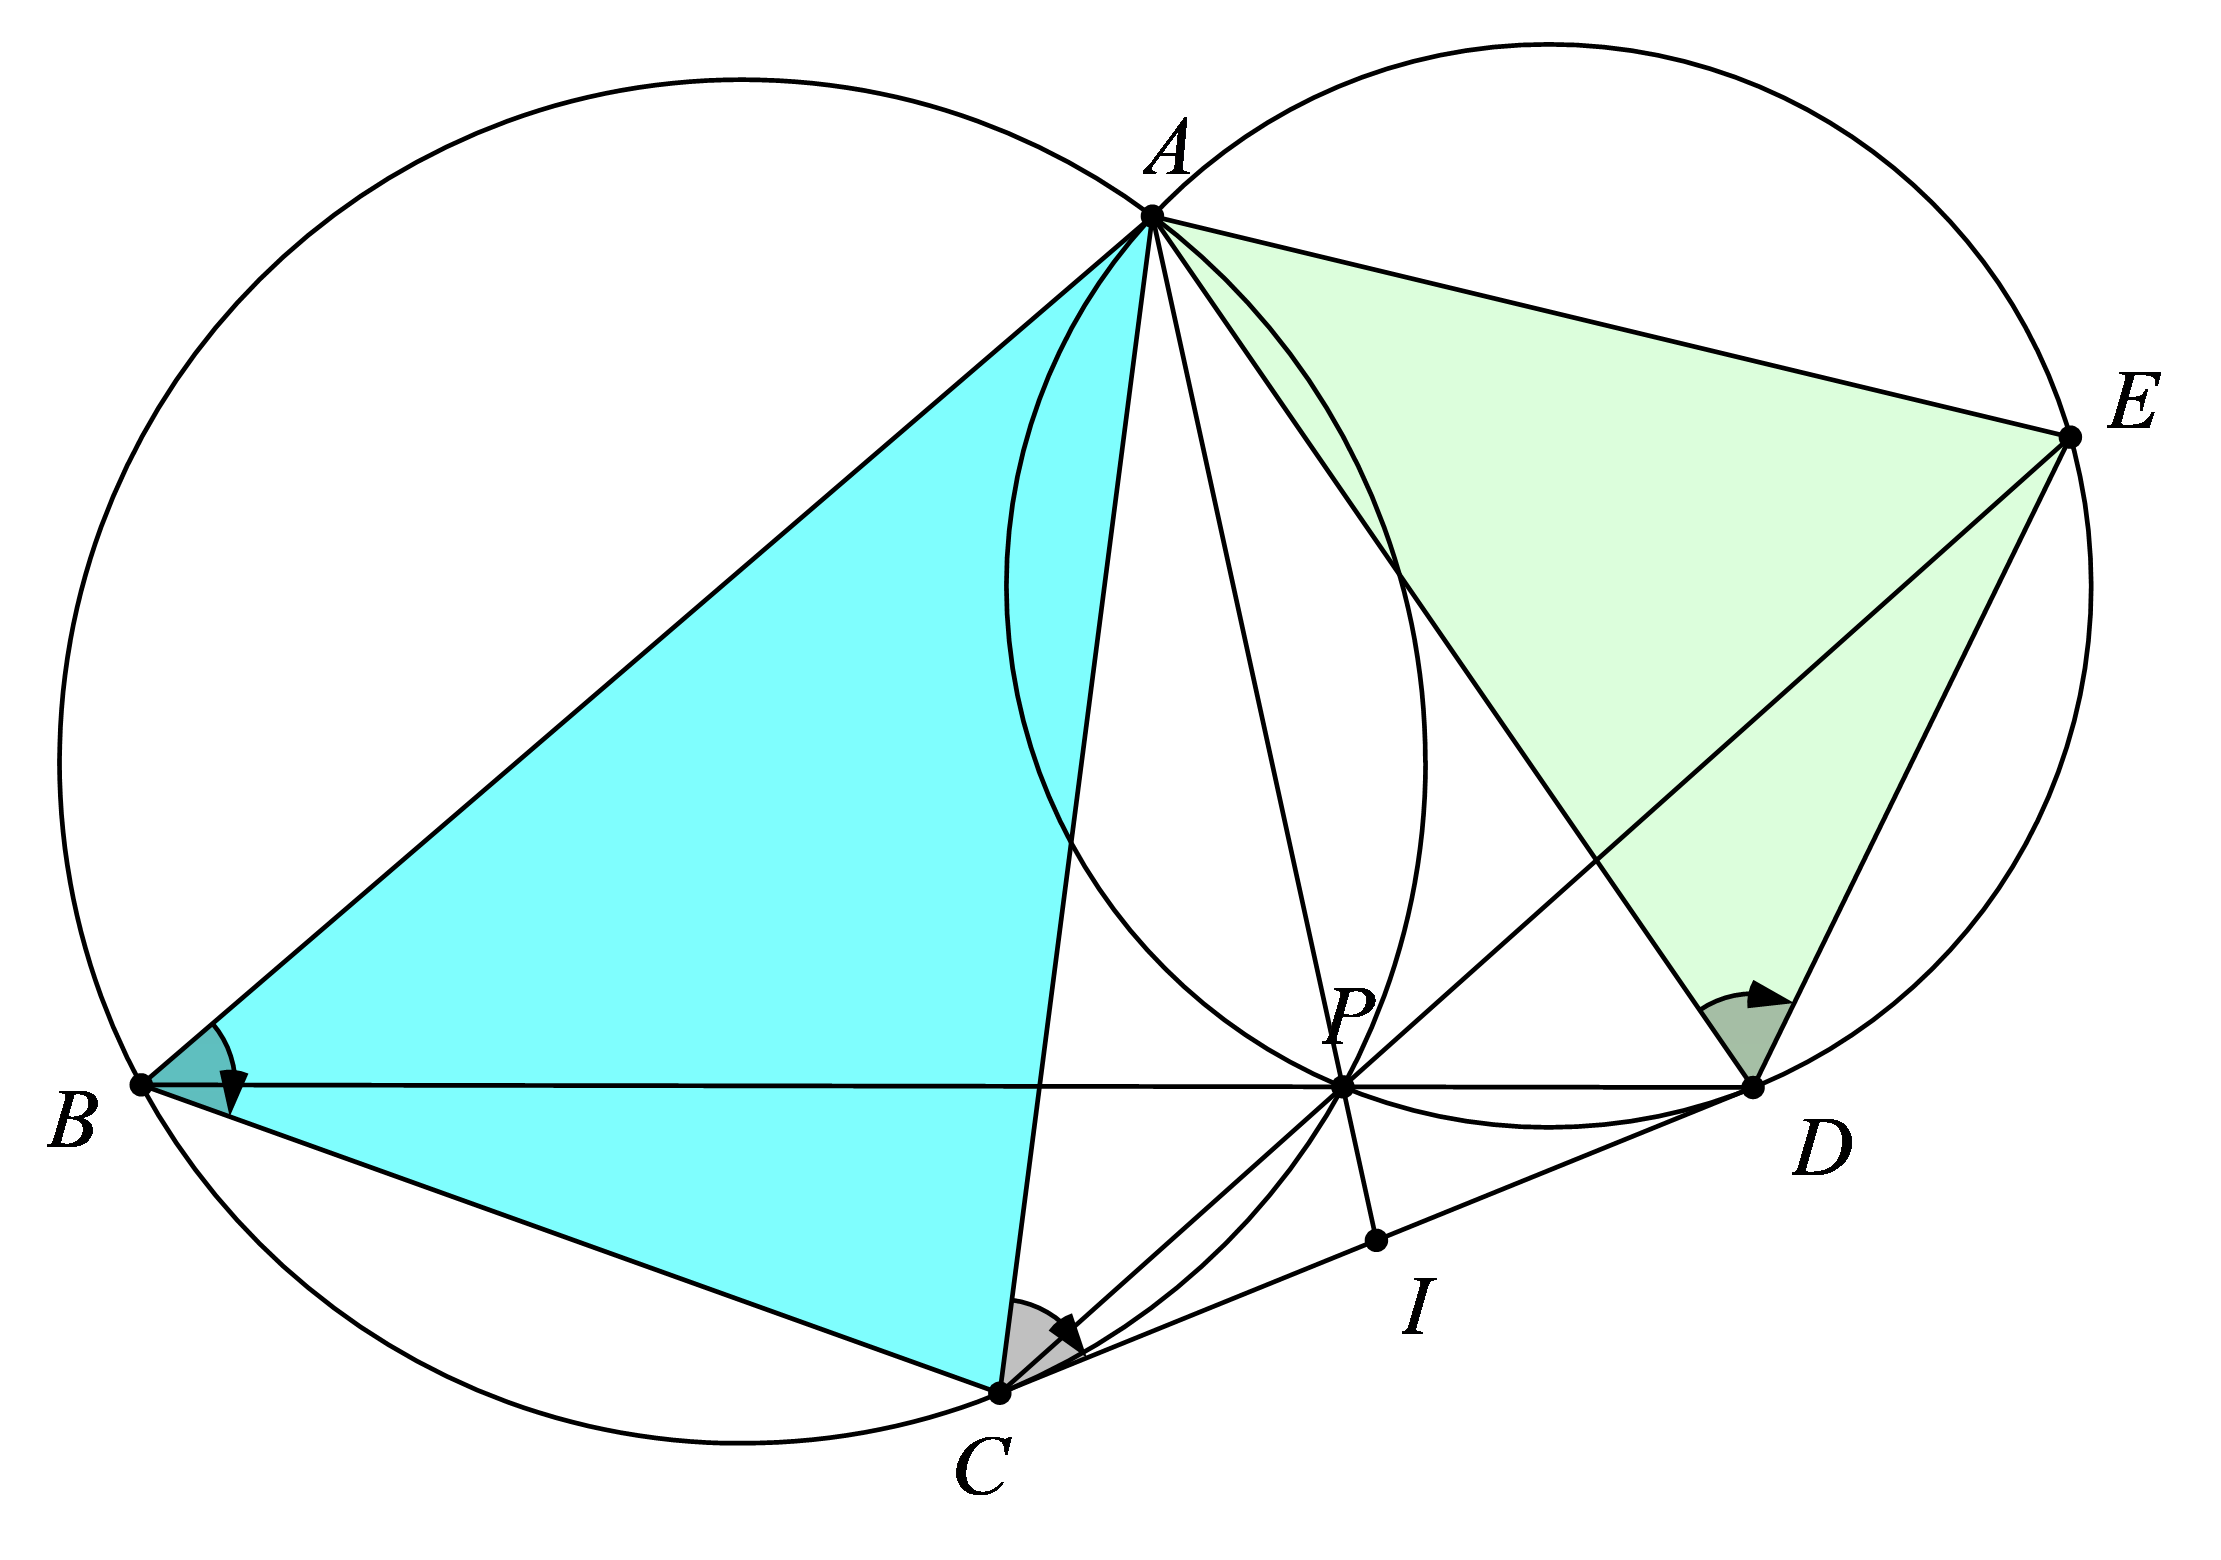
\includegraphics[width= 1\linewidth]{9}
		\vspace*{-15pt}
	\end{figure}
	\textit{Phân tích.} Trong bài toán này, dấu hiệu nhận biết việc áp dụng Bổ đề $2$ là hai đoạn thẳng $BD$ và $CE$ cắt nhau tại $P$ và các tam giác $ABC$, $ADE$ có chung đỉnh $A$ và đồng dạng với nhau. Khi đó, giao điểm thứ hai của các đường tròn $(PBC)$ và $(PDE)$ chính là tâm của phép vị tự quay. 
	\vskip 0.1cm
	\textit{Lời giải $1$.} Một mặt, theo giả thiết thì hai tam giác $ABC$ và $ADE$ đồng dạng nên có một phép vị tự quay tâm $A$ biến $B$ thành $C$, biến $D$ thành $E$, và đoạn thẳng $BD$ biến thành đoạn thẳng $CE$. Áp dụng Bổ đề $2$ cho hai đoạn thẳng $BD$ và $CE$ ta thấy rằng phép vị tự quay này có tâm là giao điểm thứ hai của các đường tròn $(PBC)$ và $(PDE)$, vì thế $A$ là giao điểm thứ hai của $(PBC)$ và $(PDE)$.
	\vskip 0.1cm
	Mặt khác, vì các tam giác $ABC,ACD,ADE$ đồng dạng (g.g) nên ta có $\angle ABC = \angle ACD, \angle ADC = \angle AED$. Do đó $CD$ là tiếp tuyến chung của hai đường tròn $(PBC)$ và $(PDE)$. Mà hai đường tròn này có trục đẳng phương là $AP$ nên nó chia đôi $CD$.
	\vskip 0.1cm
	Để so sánh với lời giải sử dụng Bổ đề 1 trên đây, chúng tôi trình bày một lời giải thứ hai.
	\textit{Lời giải $2$.} Gọi $X$ là giao điểm của $AC$ và $BD$, $Y$ là giao điểm của $AD$ và $CE$. Theo \textit{Lời giải $1$}, tồn tại phép vị tự quay $f$ tâm $A$ biến $B,\,C,\,D$ tương ứng thành $C,\,D,\,E$. Vì thế, $f$ biến các đoạn thẳng $AC$ và $BD$ tương ứng thành $AD$ và $CE$. Suy ra giao điểm của $AC$ và $BD$ biến thành giao điểm của $AD$ và $CE$, tức là $f$ biến $X$ thành $Y$.
	\begin{figure}[H]
		\vspace*{-5pt}
		\centering
		\captionsetup{labelformat= empty, justification=centering}
		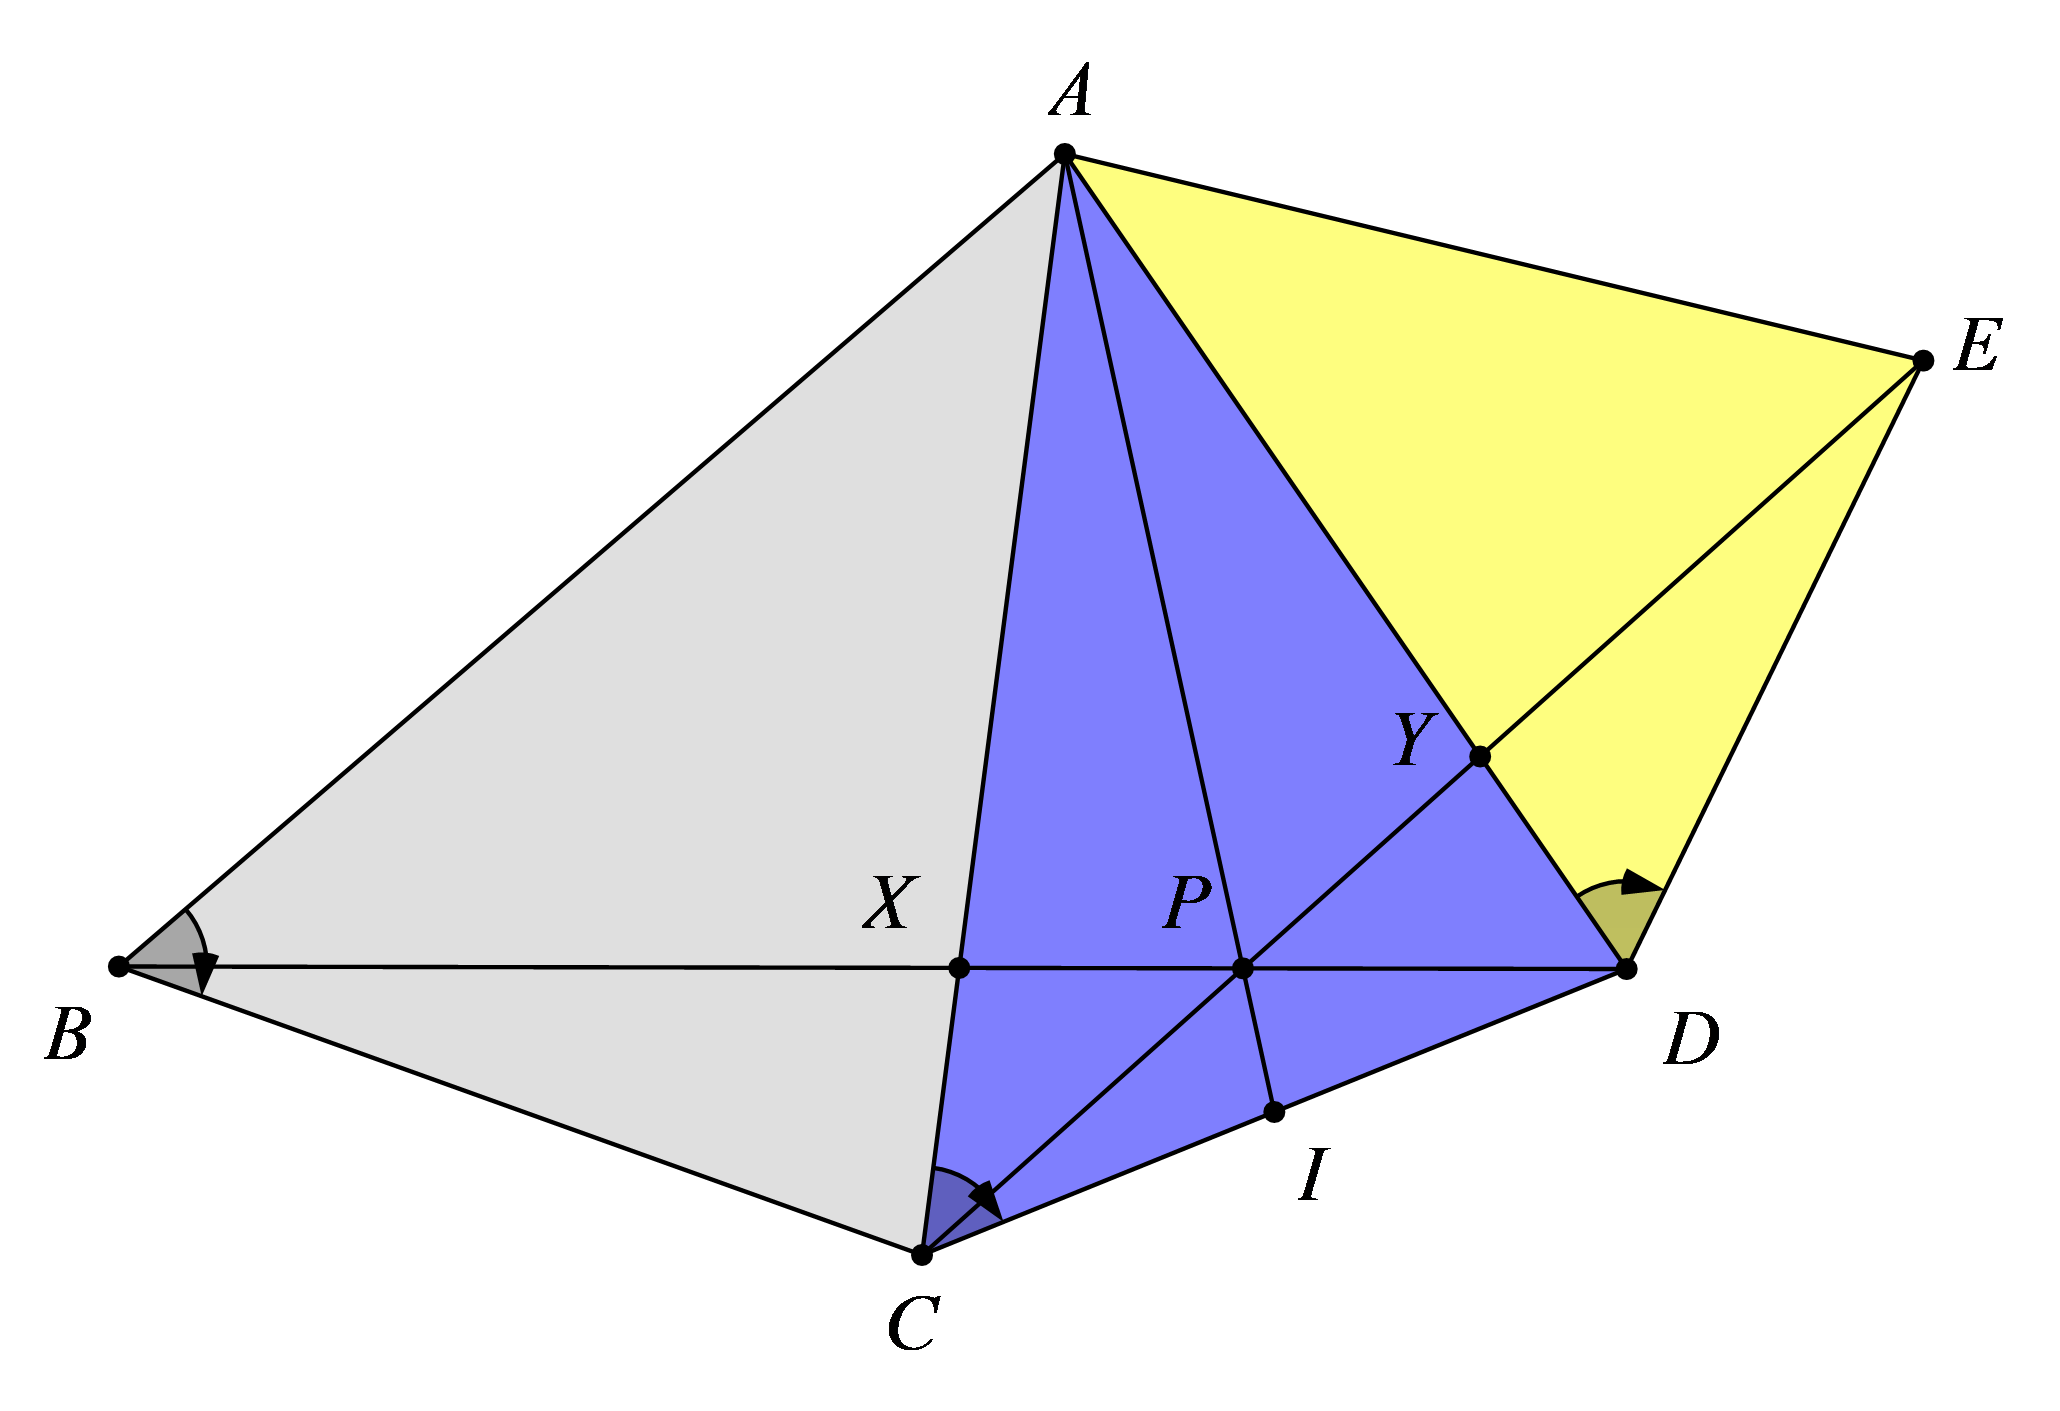
\includegraphics[width= 1\linewidth]{10}
		\vspace*{-15pt}
	\end{figure}
	Từ đó ta có
	\begin{align*}
		\dfrac{XA}{XC} = \dfrac{YA}{YD}. \tag{$*$}
	\end{align*}
	Gọi $I$ là giao điểm của $AP$ với $CD$ và áp dụng định lý Ceva cho tam giác $ACD$ với điểm đồng quy $P$, ta có
	\begin{align*}
		\frac{XA}{XC}\cdot \frac{IC}{ID}\cdot\frac{YD}{YA} = 1.
	\end{align*}
	Từ đó, kết hợp ($*$), ta suy ra $IC=ID$.
	\vskip 0.1cm
	\textit{Nhận xét.}  Lời giải $2$ không dùng đến Bổ đề về hai đoạn thẳng mà dùng đến kết quả của phép vị tự quay. Việc phát hiện ra hệ thức $(*)$ là điều không hề dễ. Theo quan sát trong thực tế dạy học của tác giả, rất ít học sinh nghĩ ra  lời giải theo hướng này. Mặt khác, sau khi biết về bổ đề hai đoạn thẳng thì đa số học sinh dễ dàng phát hiện ra dấu hiệu và áp dụng vào bài toán một cách dễ dàng.
	\vskip 0.1cm
	Bài toán sau đây được lấy từ một kỳ thi Vô địch Liên bang Nga.
	\vskip 0.1cm
	\textbf{\color{hoccungpi}Ví dụ $\pmb{5.}$} Cho tam giác nhọn $ABC$. Gọi $A_1$, $B_1$, $C_1$ tương ứng là tiếp điểm của các đường tròn bàng tiếp góc $A$ với $BC$, góc $B$ với $CA$, góc $C$ với $AB$. Các đường tròn $(AB_1C_1)$, $(BC_1A_1)$, $(CA_1B_1)$ cắt lại $(ABC)$ tại $M,N,P$. Gọi $D,E,F$ là các tiếp điểm của đường tròn nội tiếp với $BC,CA,AB$. Chứng minh rằng $MD,NE,PF$ đồng quy.
	\begin{figure}[H]
		\vspace*{-5pt}
		\centering
		\captionsetup{labelformat= empty, justification=centering}
		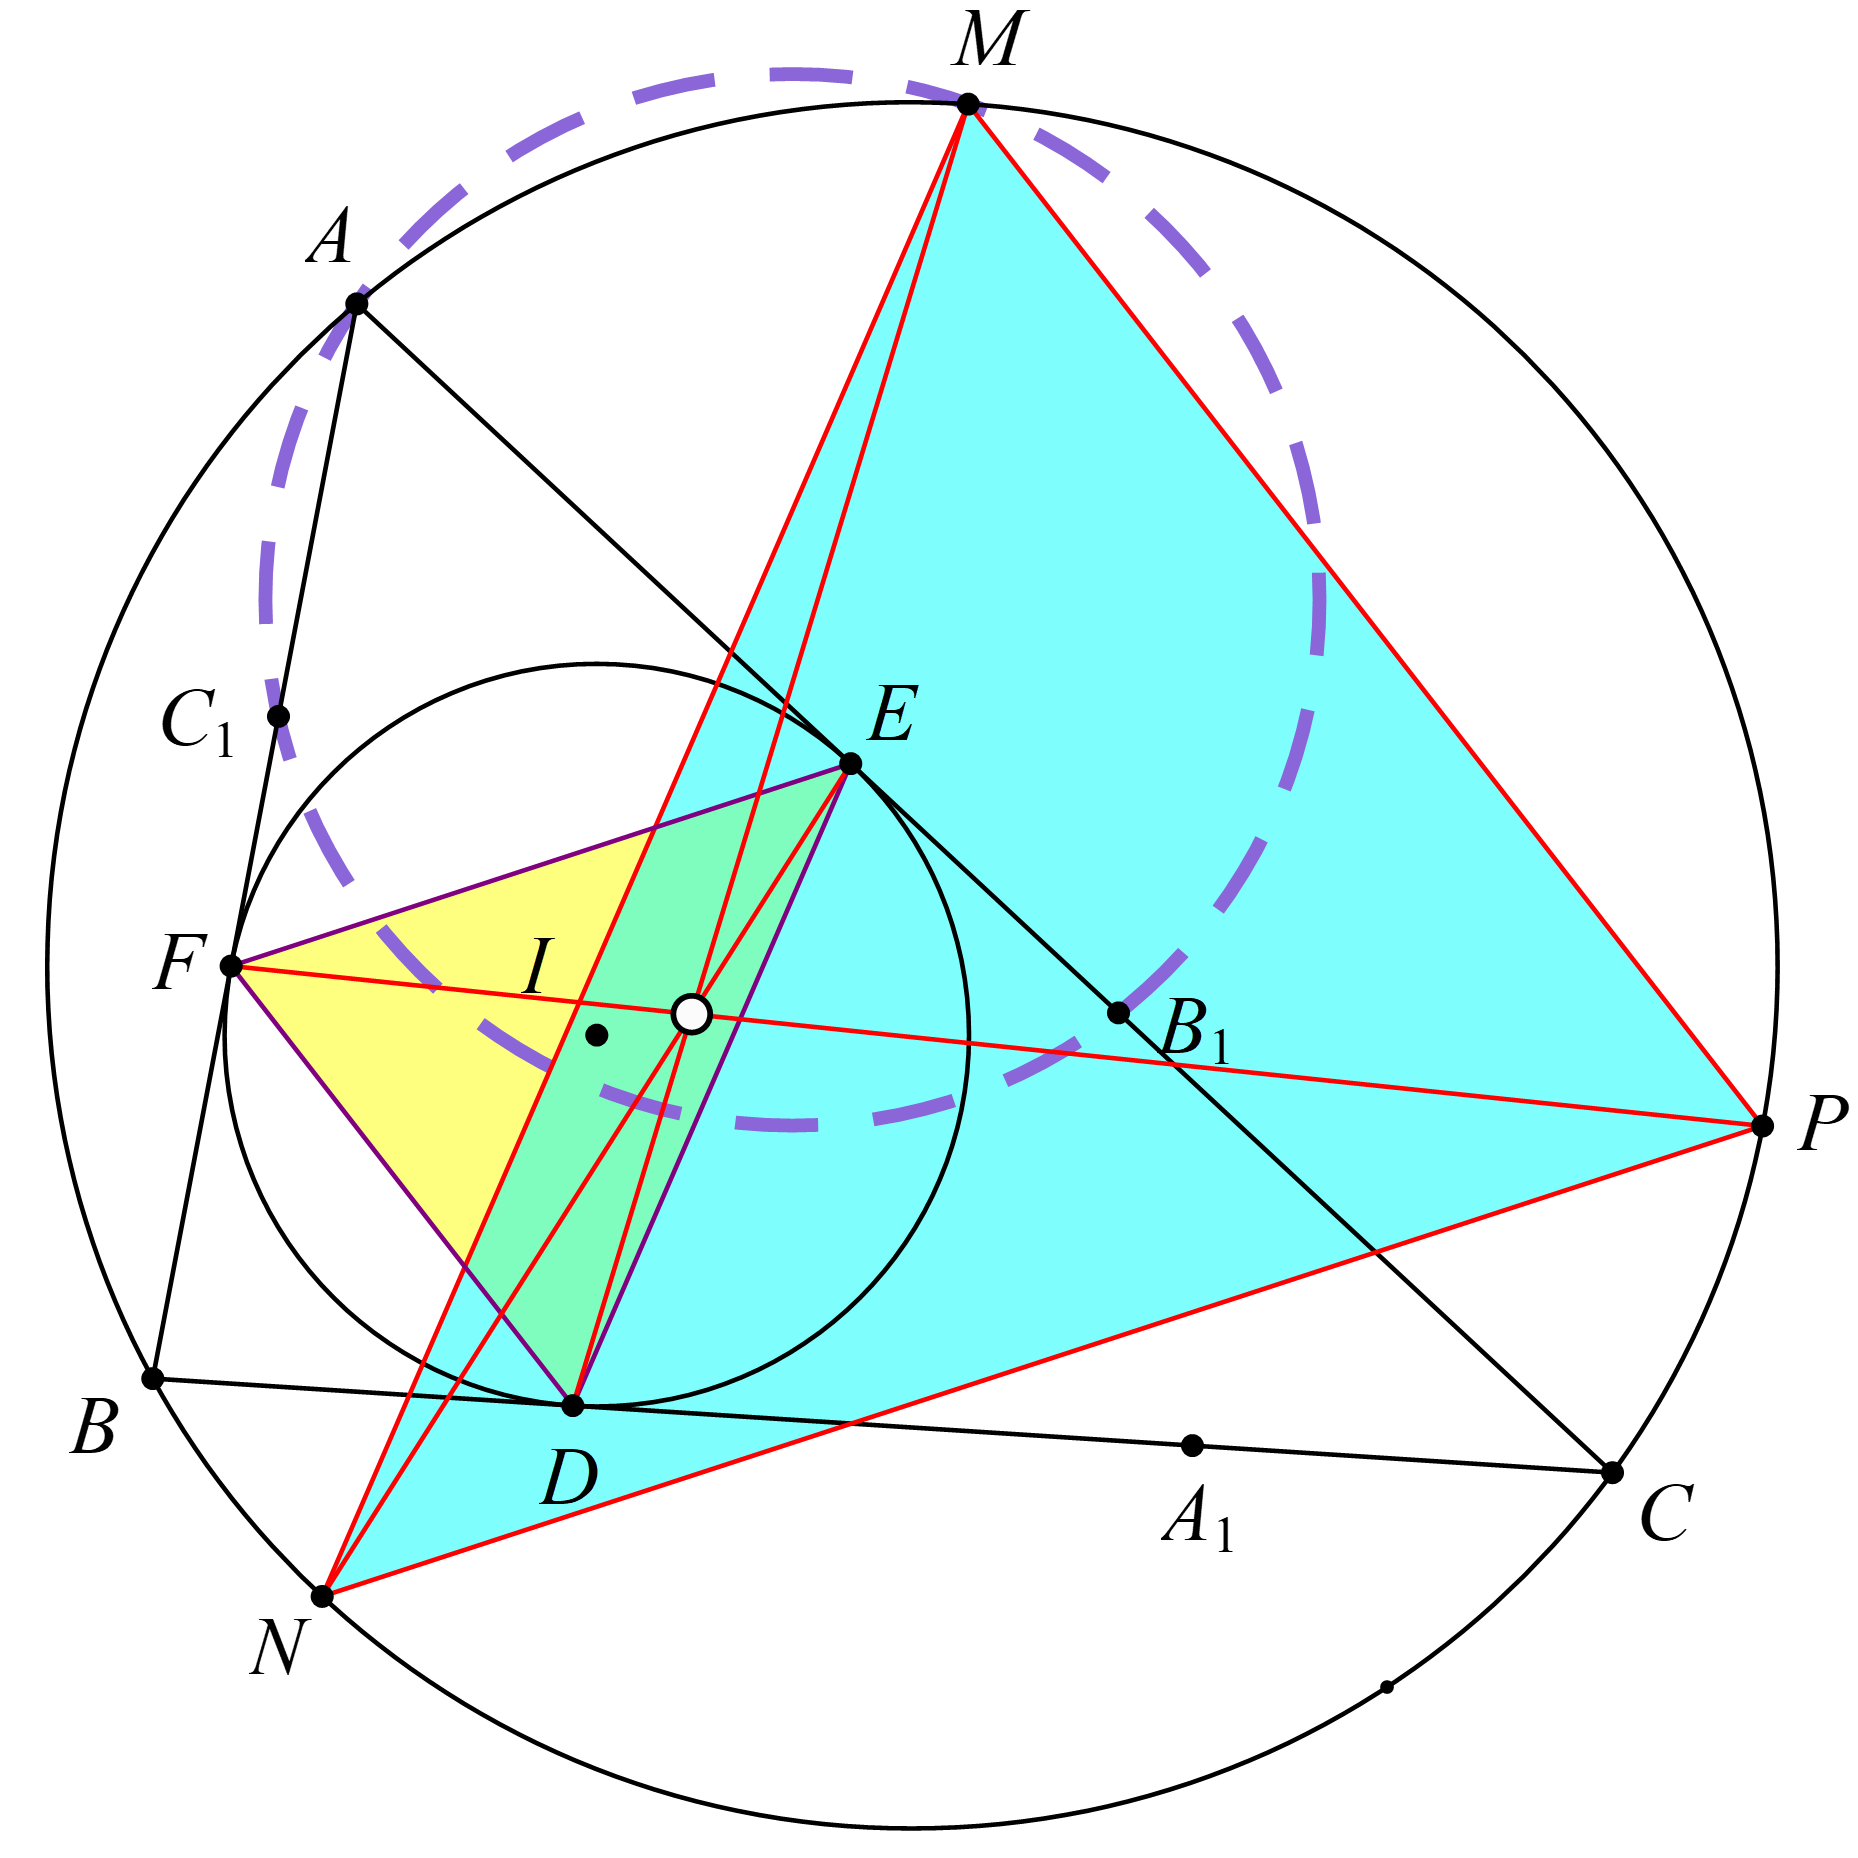
\includegraphics[width= 0.9\linewidth]{11}
		\vspace*{-10pt}
	\end{figure}
	\textit{Phân tích.} Bằng hình vẽ ta dễ phát hiện ra rằng $M,N,P$ tương ứng là các trung điểm cung $BC,CA,AB$ của đường tròn $(ABC)$ và đây là dấu hiệu để ta nghĩ đến cách tiếp cận bài toán dựa vào Bổ đề $1$. Như vậy ta phải tìm những cặp đoạn thẳng bằng nhau, tuy nhiên điều này không quá khó khi dựa vào tính chất tiếp tuyến và tiếp điểm của các đường tròn nội tiếp, bàng tiếp.
	\vskip 0.1cm
	\textit{Lời giải.} Dễ thấy $CB_1 =AE=AF=BC_1$. Áp dụng Bổ đề $1$ ta có $M$ là trung điểm cung $BC$ chứa $A$ của $(ABC)$; tương tự với $N,P.$ Ta dễ thấy rằng hai tam giác $DEF$ và $MNP$ có các cặp cạnh tương ứng song song (chẳng hạn $NP$ và $EF$ cùng vuông góc với phân giác trong góc $A$). Vì vậy tồn tại một phép vị tự biến $D,E,F$ tương ứng thành $M,N,P$. Vậy $MD,NE,PF$ đồng quy tại tâm vị tự của hai tam giác trên. 
	\vskip 0.1cm
	Bài toán sau đây được trích từ kỳ thi chọn học sinh giỏi quốc gia năm $2017$ của Việt Nam.
	\textbf{\color{hoccungpi}Ví dụ 6.} Cho tam giác $ABC$ nhọn, không cân, nội tiếp đường tròn $(O)$. Các đường cao $BE$, $CF$ cắt nhau tại $H$, $AH$ cắt $(O)$ tại $D$  (khác $A$). Các đường thẳng $DE,DF$ cắt lại $(O)$ tương ứng  $P,Q$ (khác $D$). Đường tròn $(AEF)$ cắt $(O)$ và $AO$ tương ứng tại $R,S$ (khác $A$). Chứng minh rằng $BP$, $CQ$ và $RS$ đồng quy.
	\vskip 0.1cm
	Chúng ta sẽ giới thiệu hai lời giải, một lời giải sử dụng phép biến đổi góc và lời giải còn lại sử dụng Bổ đề $2$.
	\vskip 0.1cm
	\textit{Lời giải $1$.} Gọi $X$ là trung điểm của $EF$ và $K$ là giao điểm của $AD$ và $BC$. Dễ thấy hai tam giác $BFE$ và $KHE$ đồng dạng (g.g). Gọi $T$ là trung điểm của $HE$. Khi đó, do $X$ là trung điểm $FE$ nên ta suy ra hai tam giác $BFX$ và $KHT$ đồng dạng. Vì $K$ là trung điểm $DH$ nên tam giác $KHT$ và tam giác $DHE$ đồng dạng, dẫn đến các tam giác $BFX$ và $DHE$ là đồng dạng. Suy ra  $\angle{FBX}= \angle{HDE}$, kết hợp với  $\angle{HDE}=\angle{ADP} = \angle{ABP}=\angle{FBP} $ ta được  $\angle{FBX}= \angle{FBP}.$ Từ đây ta có $B,P,X$ thẳng hàng. Tương tự ta có $C,X,Q$ thẳng hàng.
	\begin{figure}[H]
		\vspace*{-10pt}
		\centering
		\captionsetup{labelformat= empty, justification=centering}
		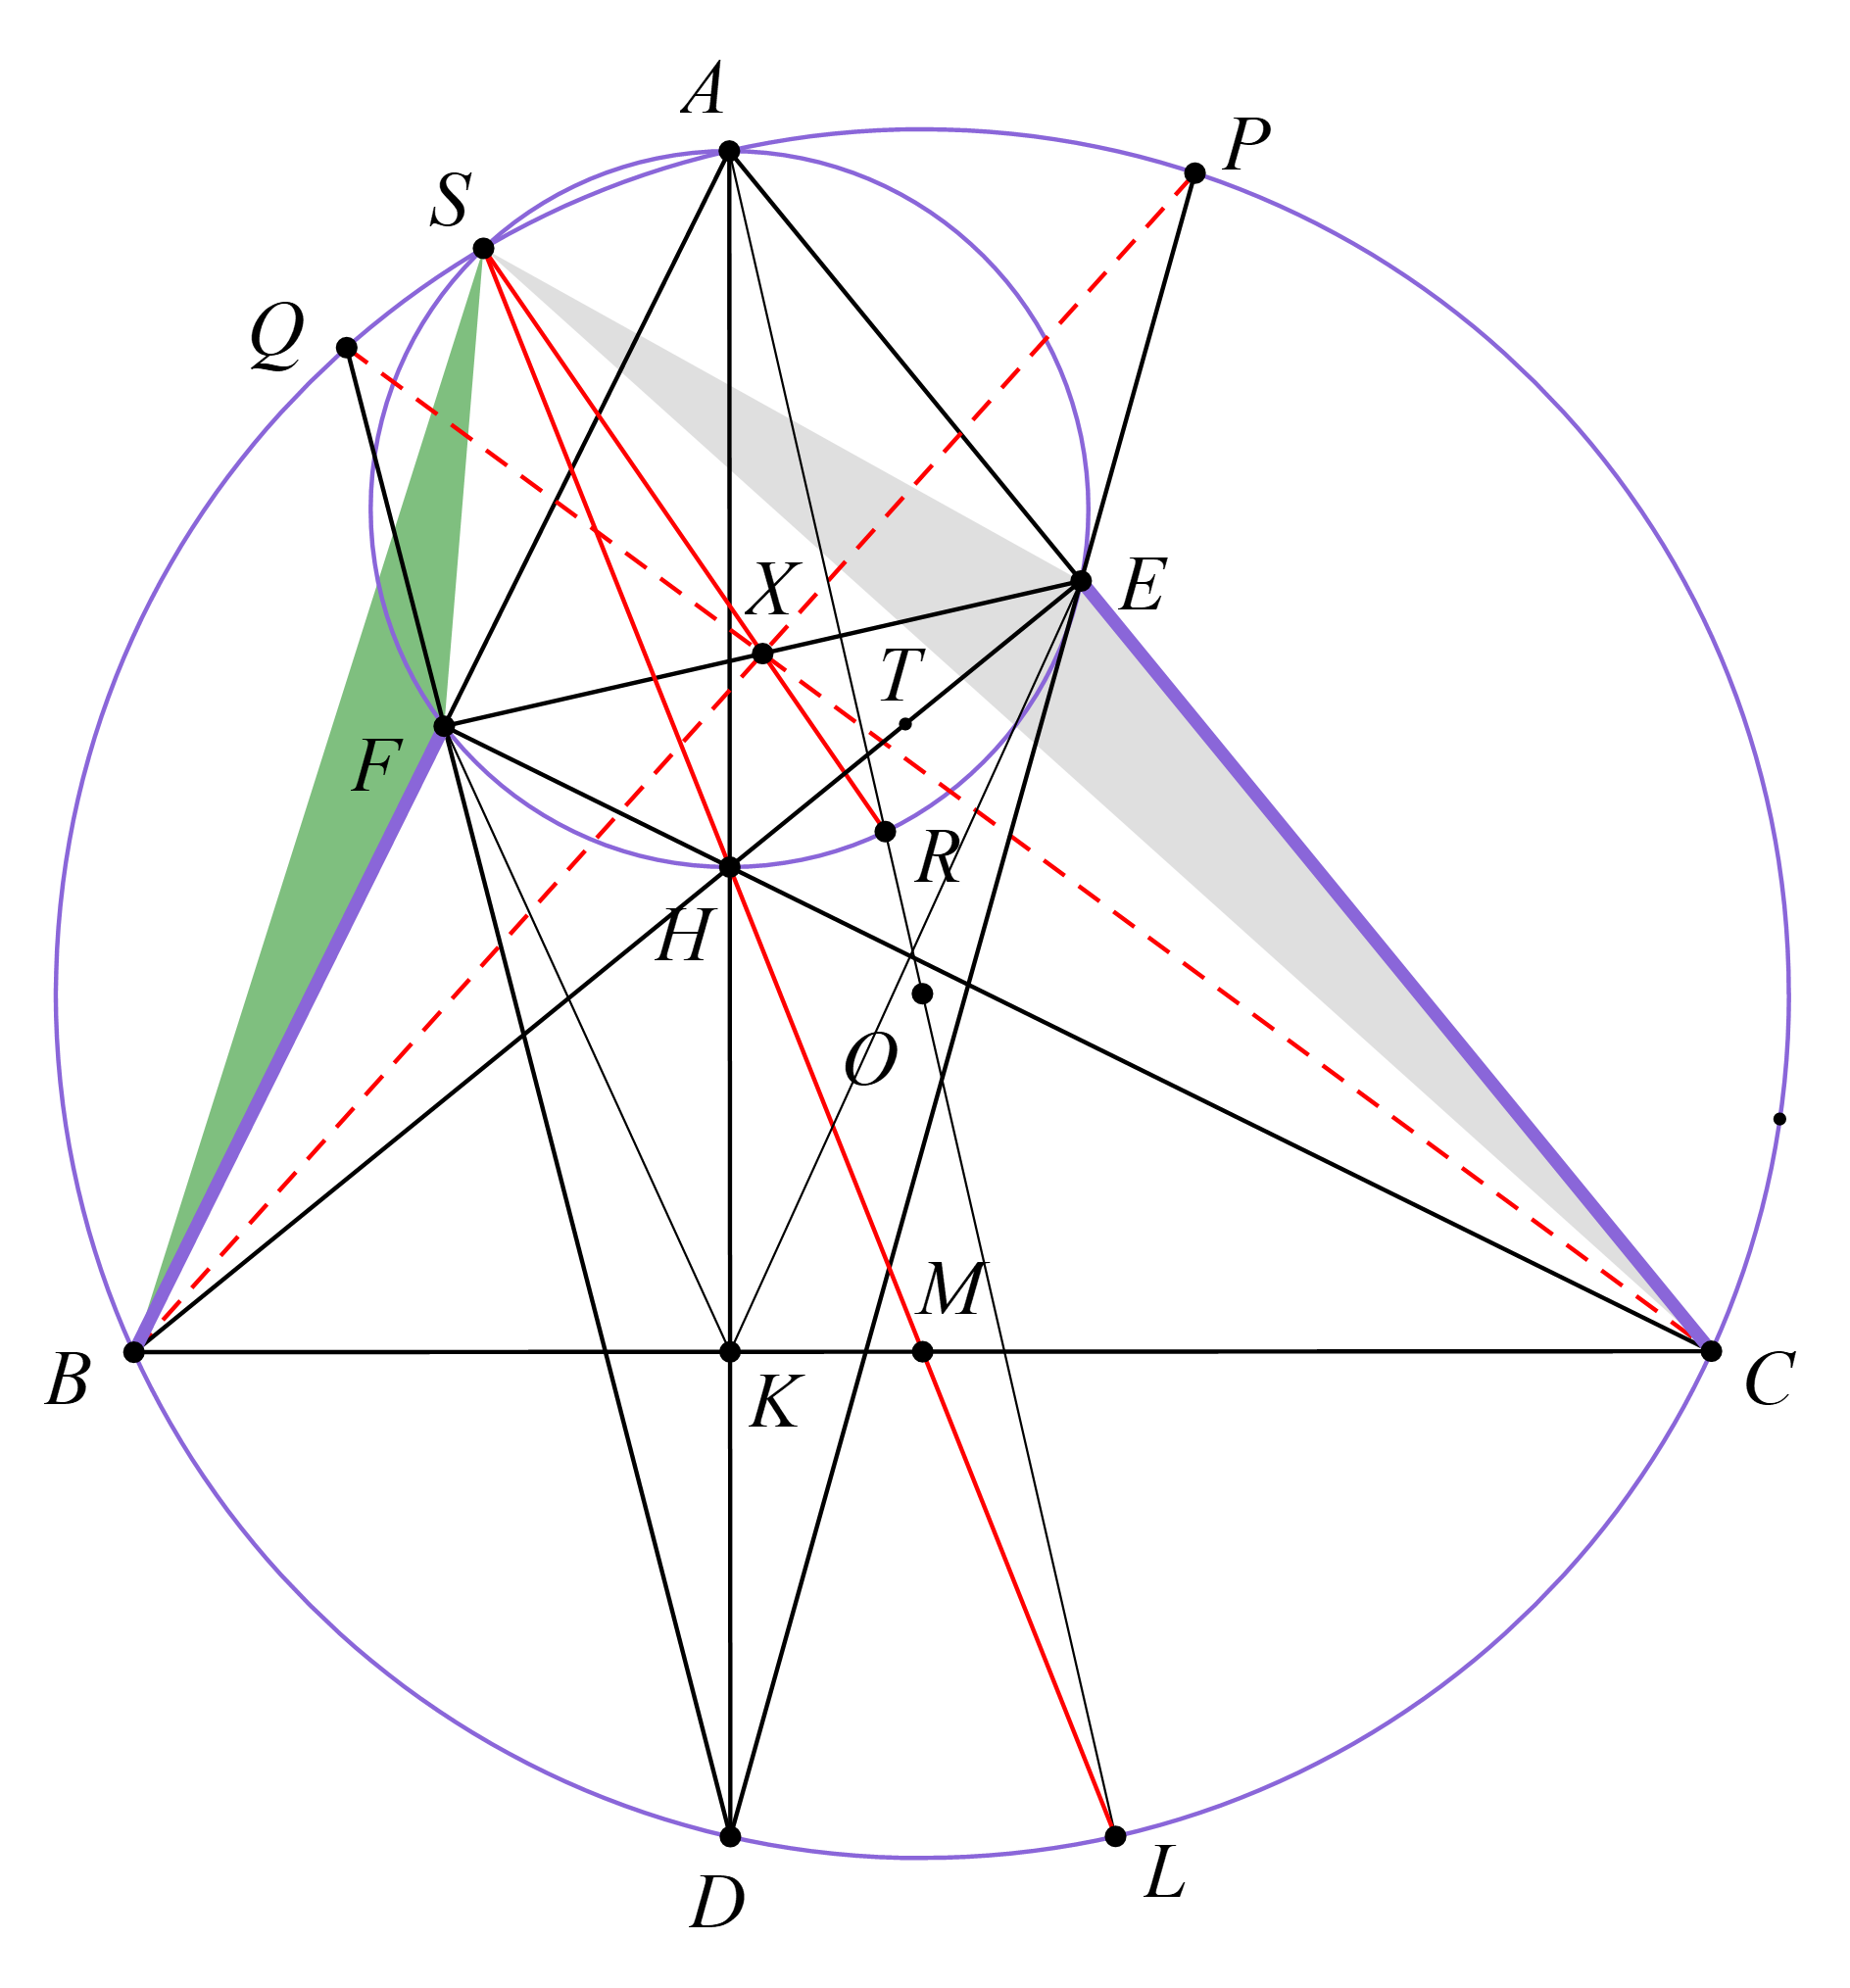
\includegraphics[width= 0.9\linewidth]{12}
		\vspace*{-15pt}
	\end{figure}
	Kẻ đường kính $AL$ của $(O)$. Dễ thấy $SH$ đi qua $L$ và do tứ giác $HBLC$ là hình bình hành nên $HL$ đi qua trung điểm $M$ của $BC$. Dễ thấy hai tam giác $SEC$ và $SFB$ đồng dạng (g.g) nên hai tam giác $SEF$ và $SCB$ đồng dạng (c.g.c). Mà hai tam giác này có các trung tuyến tương ứng là $SX$ và $SM$ nên ta suy ra $\angle FSX =  \angle BSM$. Tương tự, do hai tam giác $SFB$ và $SRL$ đồng dạng (g.g) nên hai tam giác $SFR$ và $SBL$ đồng dạng (c.g.c), dẫn đến  $\angle FSR=\angle BSL=\angle BSM=\angle FSX$. Từ đó suy ra $S,X,R$ thẳng hàng. Vậy, $SR,BP,CQ$ đồng quy tại trung điểm $X$ của $EF$.
	\vskip 0.1cm
	\textit{Lời giải $2$.} Gọi $X$ là trung điểm của $EF$. Tương tự như \textit{Lời giải $1$}, ta cũng chứng minh được $BP$ và $CQ$ đi qua $X$. Ta cần chứng minh $SR$ cũng đi qua $X$. Kẻ đường kính $AL$. Áp dụng Bổ đề $2$ cho hai đoạn thẳng $BF$ và $CE$ (và để ý rằng chúng cắt nhau tại $A$) ta suy ra $S$ là tâm của phép vị tự quay $f$ biến đoạn $FE$ thành đoạn $BC$ và biến $X$ biến thành $M$. Từ đó $f$ biến $(AEF)$ thành $(ABC)$. Kết hợp với việc $A,R,L$ thẳng hàng, ta suy ra $f$ biến $R$ thành $L$. Các điểm $S,L,M$ tương ứng biến thành $S,R,X$. Mà  $S,L,M$ thẳng hàng nên $S,R,X$ thẳng hàng. Vậy, $SR,BP,CQ$ đồng quy tại $X$.
	\vskip 0.1cm
	\textit{Nhận xét.} Ở lời giải thứ nhất, để chứng minh $SR$ đi qua $X$, ta đã sử dụng phép biến đổi góc dựa vào việc tìm ra những cặp tam giác đồng dạng khá phức tạp. Tuy nhiên ở lời giải thứ hai thì việc áp dụng Bổ đề $2$ cho ta cách tiếp cận dễ dàng hơn nhiều. Dấu hiệu nhận biết ở đây là việc hai đường tròn $(O)$ và $(AEF)$ cắt nhau tại $ A,S$ và có $BF$ cắt $CE$ tại $A$.
	\vskip 0.1cm 
	$\pmb{2.3.}$ \textbf{\color{hoccungpi} Chứng minh đường thẳng hoặc đường tròn luôn qua điểm cố định}
	\vskip 0.1cm
	Bài toán sau đây được lấy từ đề thi Toán quốc tế (IMO) năm $2005$.
	\vskip 0.1cm
	\textbf{\color{hoccungpi}Ví dụ $\pmb{7}$.} Cho $ABCD$ là tứ giác lồi có $AD=BC$ và $AD,BC$ không song song. Gọi $E,F$ tương ứng  là các điểm trên $BC,AD$ sao cho $BE=DF$. Các đường thẳng  $AC$ và $BD$ cắt nhau tại $P$, các đường thẳng $BD$ và $EF$ cắt nhau tại $Q$, các đường thẳng $EF$ và $AC$ cắt nhau tại $R$. Chứng minh rằng, khi $E$ và $F$ thay đổi, đường tròn $(PQR)$ đi qua một điểm cố định khác $P$.
	\begin{figure}[H]
		\vspace*{-5pt}
		\centering
		\captionsetup{labelformat= empty, justification=centering}
		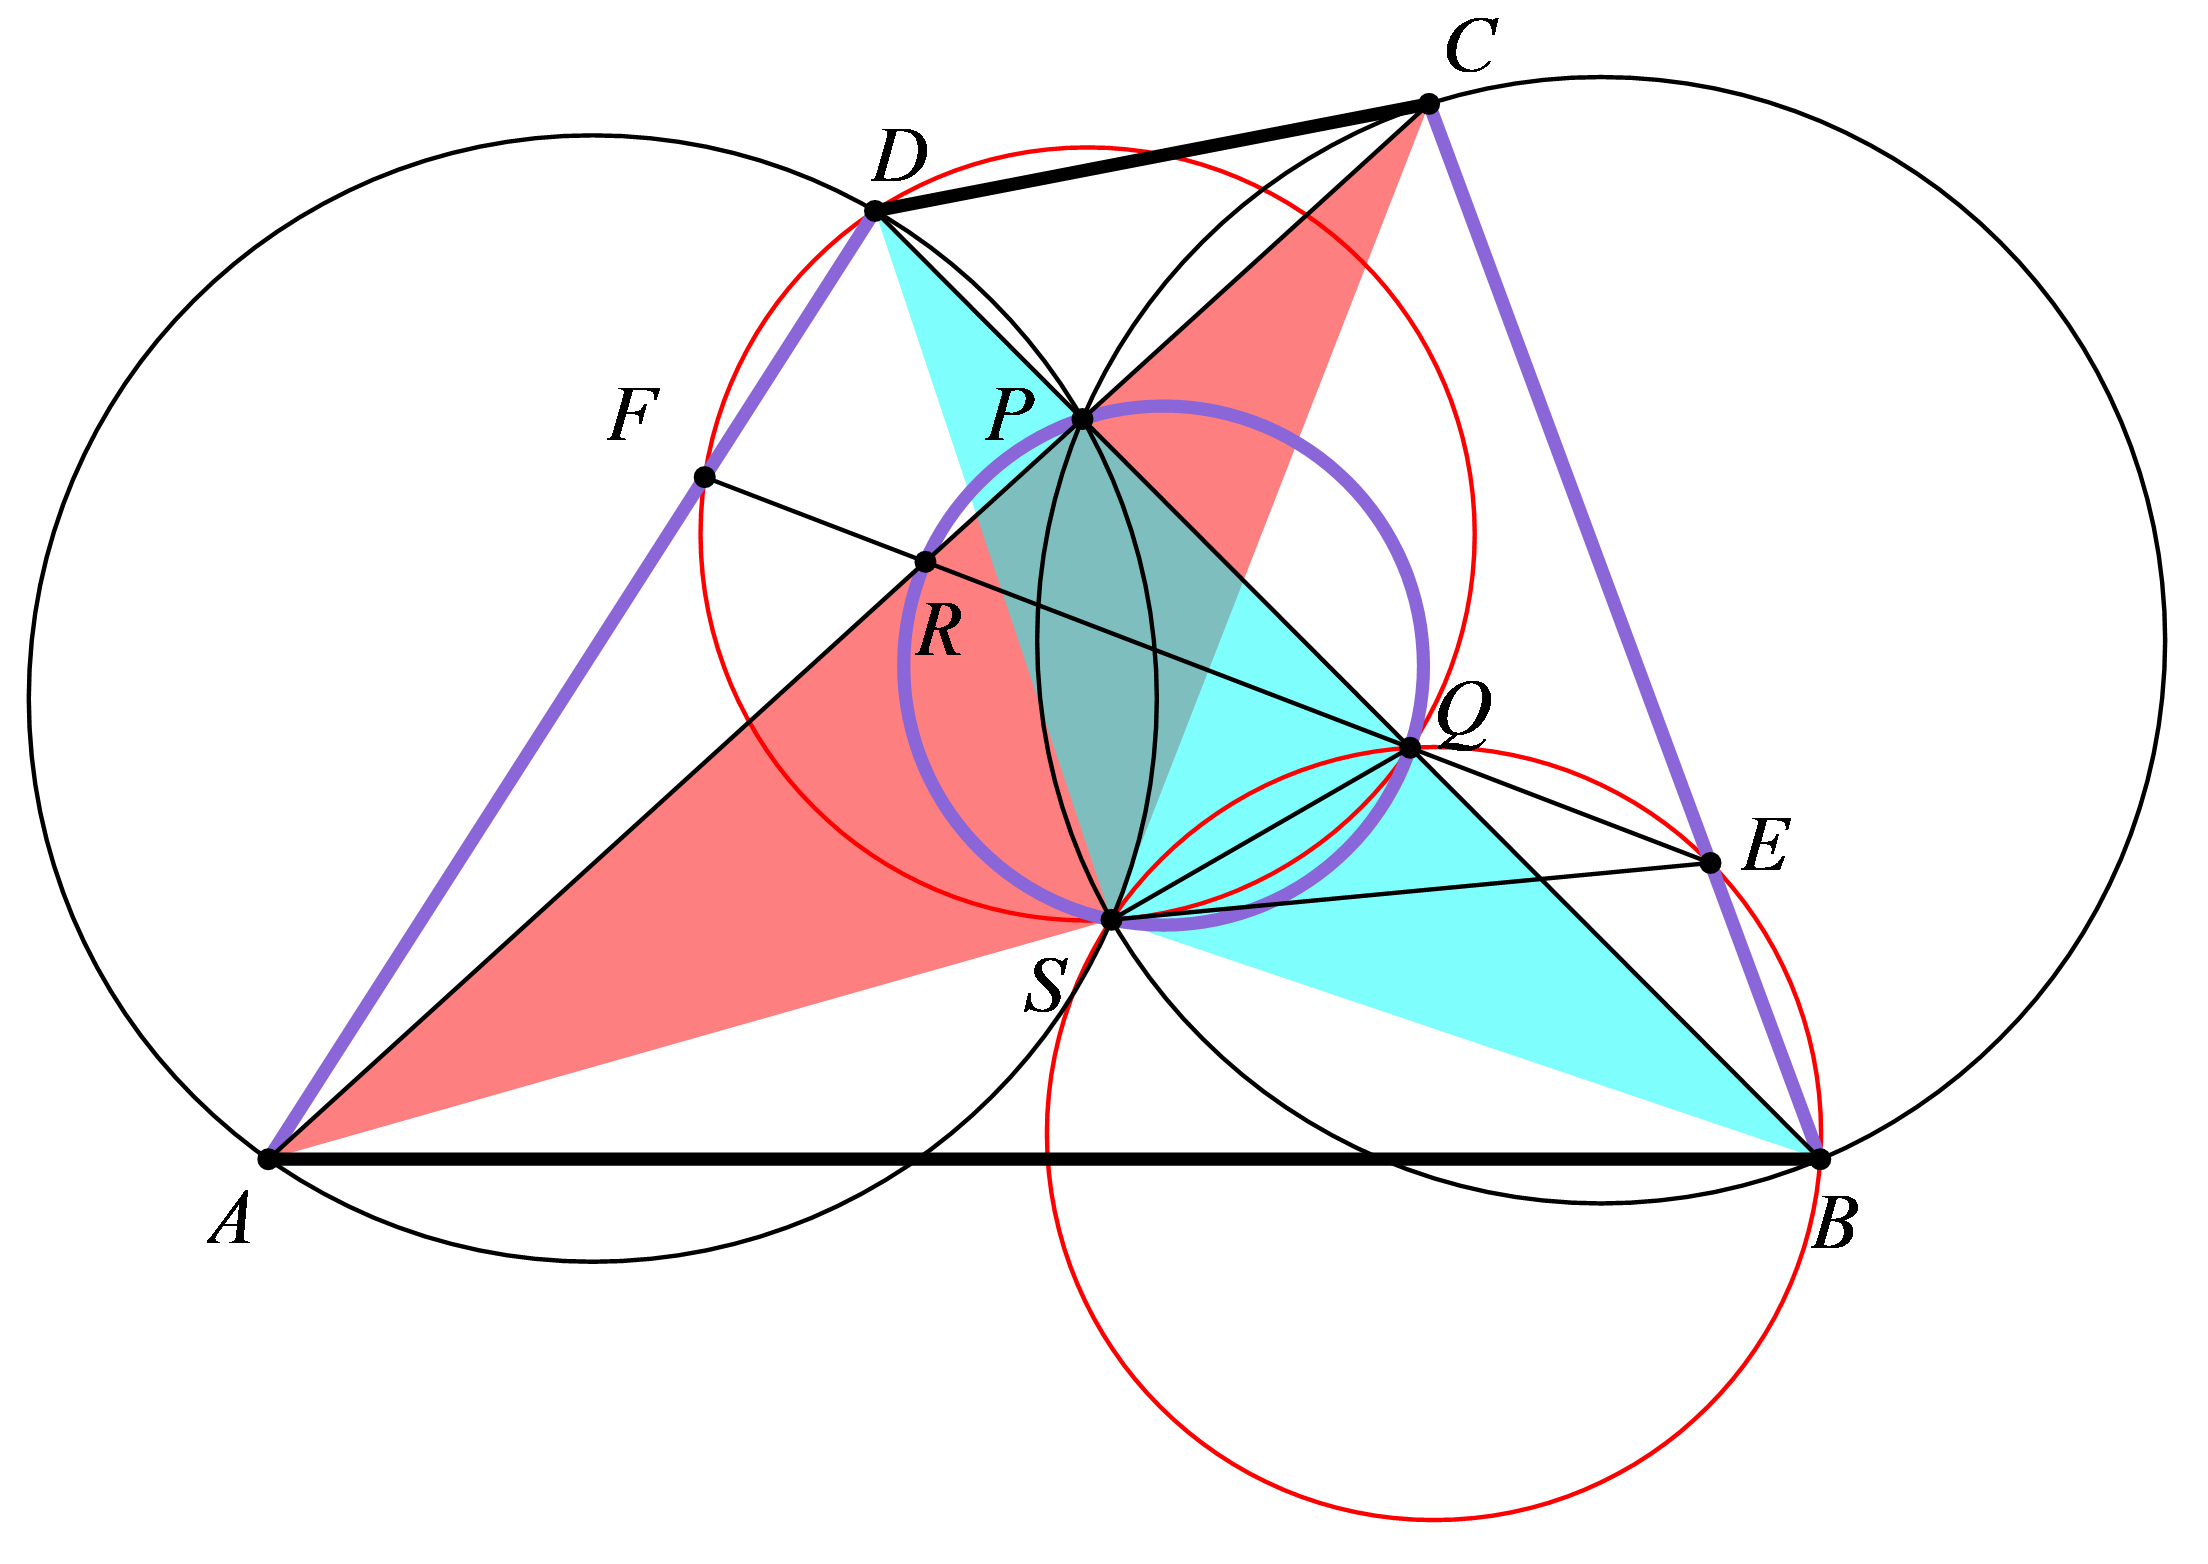
\includegraphics[width= 1.02\linewidth]{14}
		\vspace*{-15pt}
	\end{figure}
	\textit{Lời giải $1$.} Theo Bổ đề $1$, áp dụng cho hai đoạn thẳng $AD=BC$ có $AC$ cắt $BD$ tại $P$,  ta có giao điểm $S$ của hai đường tròn $(PAD)$ và $(PBC)$ là tâm phép quay (góc  $ \angle BSD$) biến $A$ thành $C$ và biến $D$ thành $B$, do đó ta có các tam giác cân $SAC,SBD$ đồng dạng. Vì $FD/FA=EB/EC$ nên phép quay này biến $F$ thành $E$, do đó ta có $SF=SE$ và $(FS, FR)=(FS, FE)=(AS, AC)=(AS, AR)\,\,\,(\bmod \pi)$. Do đó $A,S, R, F$ đồng viên. Tương tự, $B, E, Q, S$ đồng viên và $D, F, S, Q$ đồng viên. Từ đó $(RS, RP)=(FS, FA)=(FS, FD)=(QS, QP)\,\,\,(\bmod \pi)$. Suy ra $(PQR)$ đi qua điểm $S$ cố định.
	\vskip 0.1cm
	\textit{Lời giải $2$.} Theo Bổ đề $2$, tồn tại phép vị tự quay $f$ biến $A$ thành $C$ và biến $D$ thành $B$. Khi đó $f$ biến $ F$ thành $E$ (do $FD/FA=EB/EC$), và đoạn $DF$ biến thành đoạn $BE$. Do đó hai tứ giác $ACBD$ và $EFDB$ có chung điểm Miquel. Tâm của phép vị tự quay $f$ là giao điểm thứ hai $S$ của hai đường tròn $(PAD)$ và $(PCB)$, cũng là điểm Miquel chung của các tứ giác toàn phần $ACBD$ và $EFDB$. Do đó $S$ thuộc các đường tròn $(QEB)$ và $(QFD)$. Dễ thấy $S$ cũng là điểm Miquel chung của các tứ giác toàn phần $DFRP$ và $CEQP$, do đó $S$ thuộc $(PQR)$. Vì các đường tròn $(PAD)$ và $(PBC)$ cố định nên $S$ cố định. Vậy, đường tròn $(PQR)$ luôn đi qua điểm $S$ cố định. 
	\begin{figure}[H]
		%		\vspace*{-5pt}
		\centering
		\captionsetup{labelformat= empty, justification=centering}
		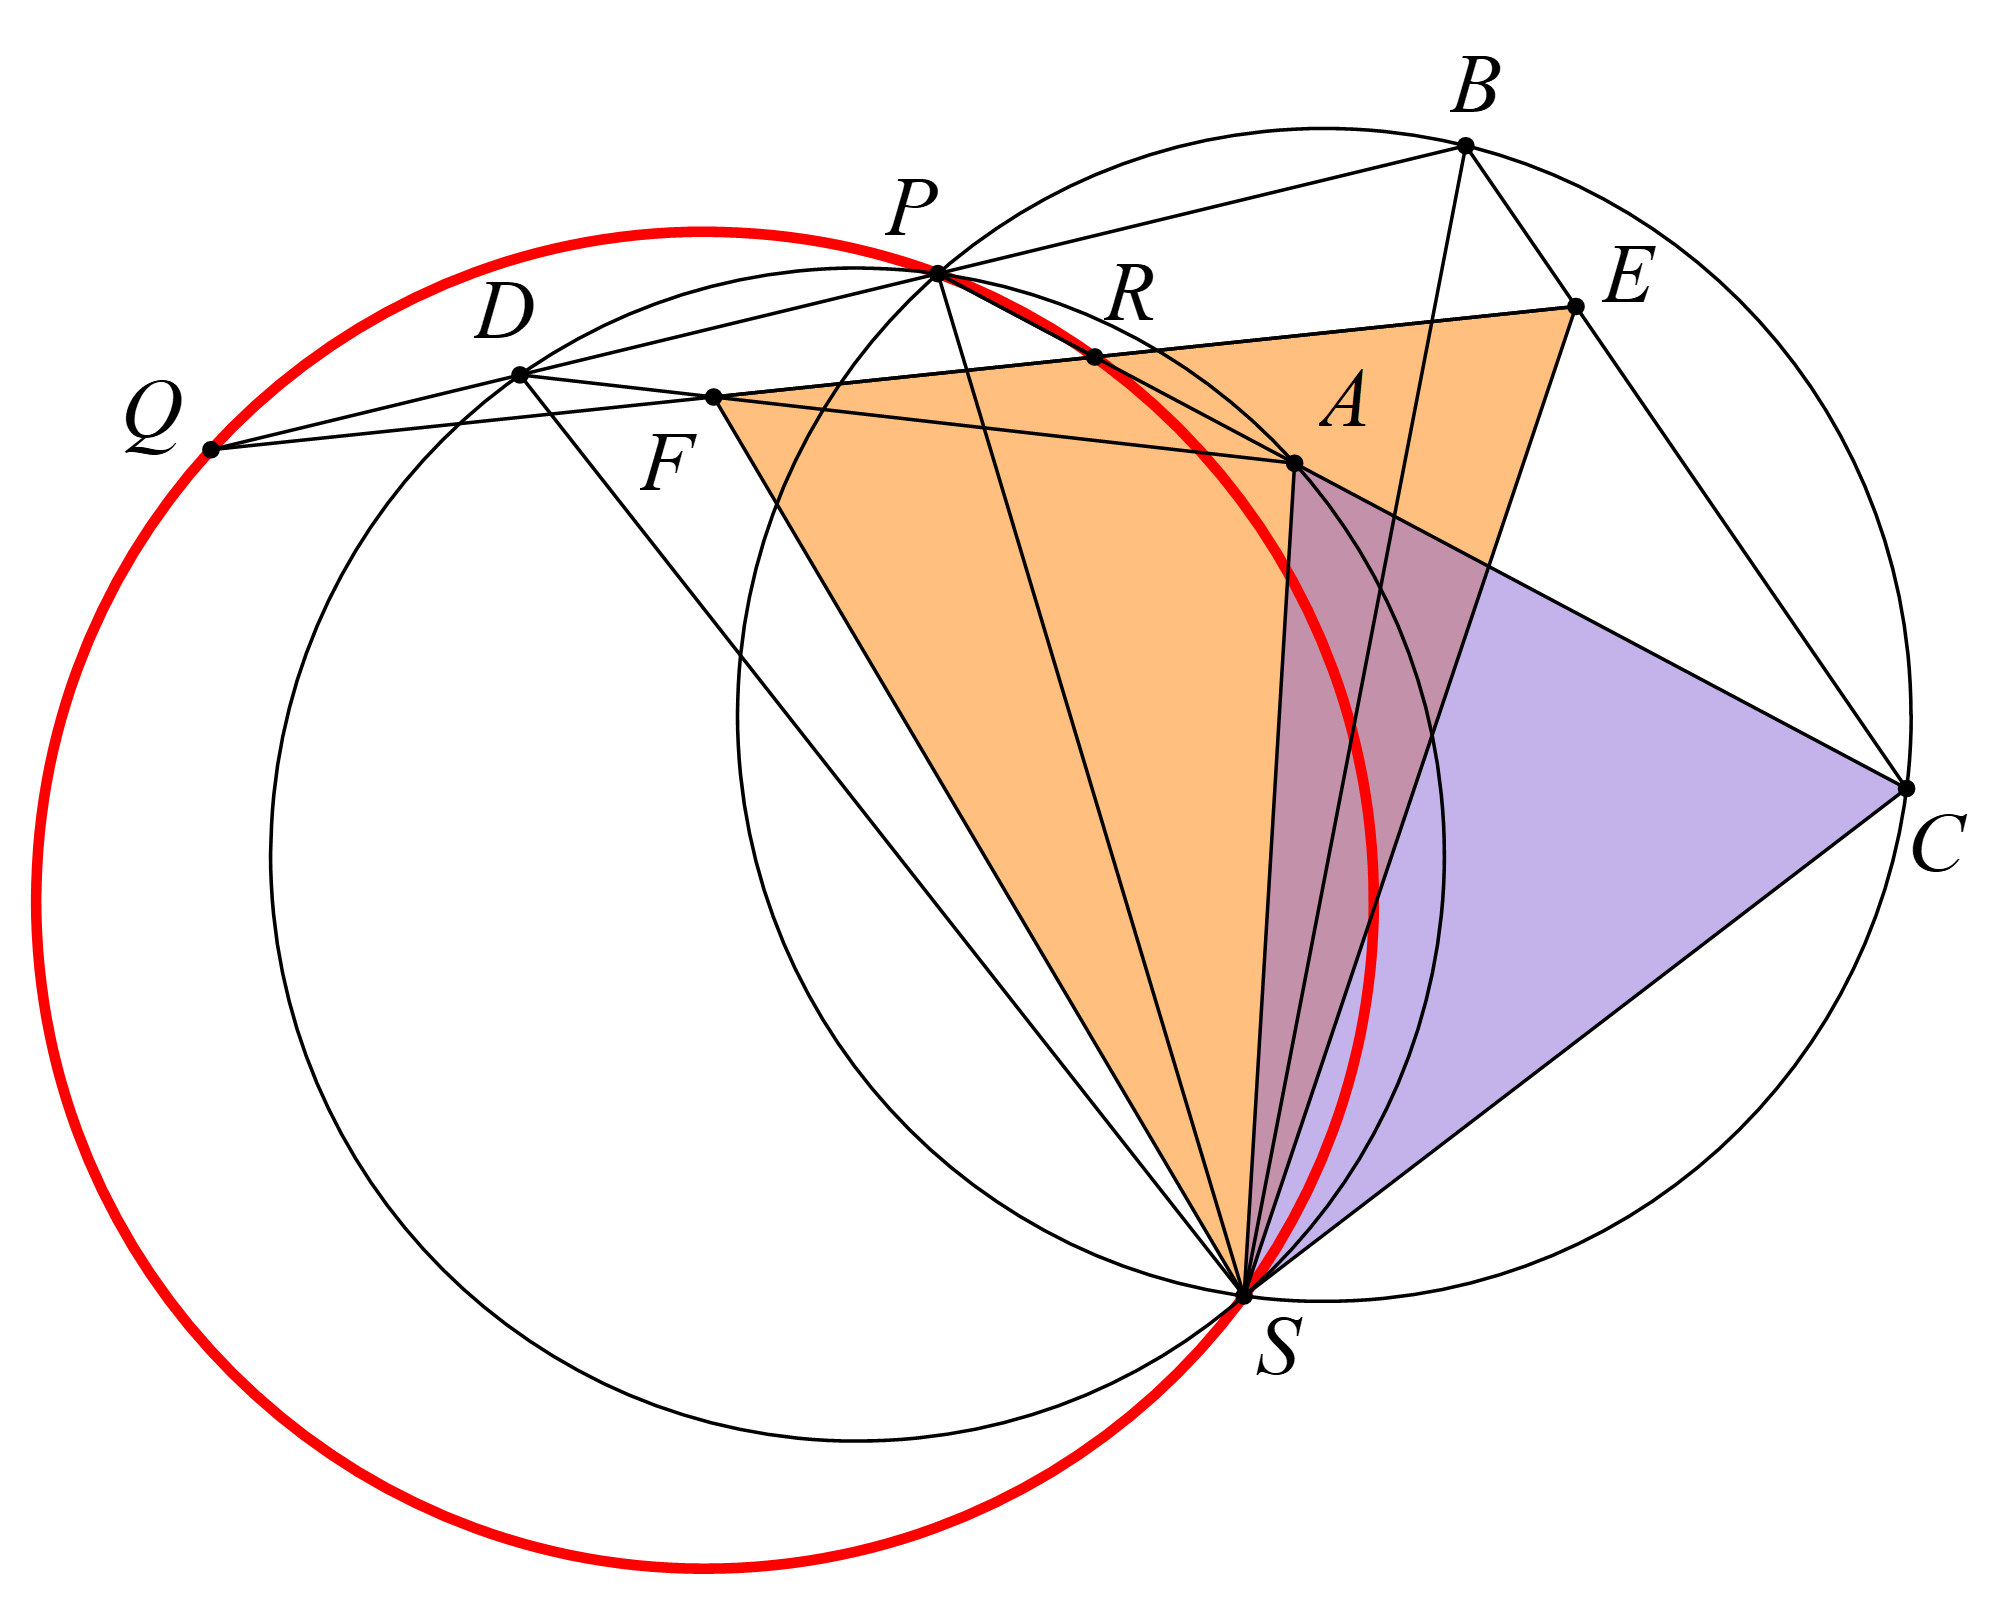
\includegraphics[width= 1\linewidth]{15}
		\vspace*{-10pt}
	\end{figure}
	\textit{Nhận xét.} $1)$ Điều thú vị là đối với bài toán này lại, chúng ta vừa có thể áp dụng Bổ đề $1$, vừa có thể áp dụng Bổ đề $2$ để giải. Điều đó cho thấy sự đa dạng và phạm vi vận dụng rộng rãi của hai bổ đề mà chúng ta đã đề cập. Trong bài toán trên, dấu hiệu để phát hiện và tiếp cận theo hướng Bổ đề $1$  là sự xuất hiện của hai đoạn thẳng bằng nhau. Mặt khác, dấu hiệu để tiếp cận và vận dụng bổ đề $2$ là có mô hình hai đoạn thẳng $AC$ và $BD$ cắt nhau tại $P$, đồng thời hai đường tròn $(PAD)$, $(PBC)$ cắt nhau tại $P$ và $S$. Hơn nữa, bài toán cũng xuất hiện hai điểm $E,F$ chia các đoạn thẳng với tỷ lệ bằng nhau nên ta nghĩ đến phép vị tự quay biến $F$ thành $E$; tâm của phép vị tự quay chính là điểm $S$.
	\vskip 0.1cm
	$2)$ Nếu thay giả thiết tứ giác $ABCD$ lồi thành bốn điểm $A, B, C, D$ bất kỳ ta vẫn thu được kết luận tương tự và các lời giải trên vẫn còn đúng.
	\vskip 0.1cm
	\textbf{\color{hoccungpi}Ví dụ $\pmb{8.}$} Cho tam giác $ABC$ nội tiếp đường tròn $(O)$ cố định với $B,C$ là các điểm cố định và điểm $A$ thay đổi trên $(O)$. Các đường cao $AD,BE,CF$ đồng quy tại $H,BO$ và $CO$ tương ứng cắt $DF,DE$ tại $K,L,KL$ cắt $EF$ tại $P$. Chứng minh rằng đường tròn $(PEL)$ luôn qua một điểm cố định.
	\vskip 0.1cm
	\textit{Phân tích.} Để ý rằng các điểm $E,F,K,L$ cùng với $P,D$ lập thành một tứ giác toàn phần, vì vậy khi xét điểm cố định mà đường tròn $(EPL)$ đi qua, ta quan tâm đến điểm Miquel của tứ giác toàn phần $EFKLPD$. Lại có $(EFD)$ chính là đường tròn Euler của tam giác $ABC$, và trung điểm $M$ của $BC$ là trung điểm cung $EF$ chứa $D$ của đường tròn này. Như vậy, ta chỉ cần chứng minh $M$ chính là điểm Miquel của tứ giác toàn phần đã nêu. Để chỉ ra điều đó, ta đưa về mô hình hai đoạn thẳng bằng nhau và áp dụng Bổ đề $1$. Từ đó ta có thể tiếp cận bài toán như sau.
	\begin{figure}[H]
		\vspace*{-5pt}
		\centering
		\captionsetup{labelformat= empty, justification=centering}
		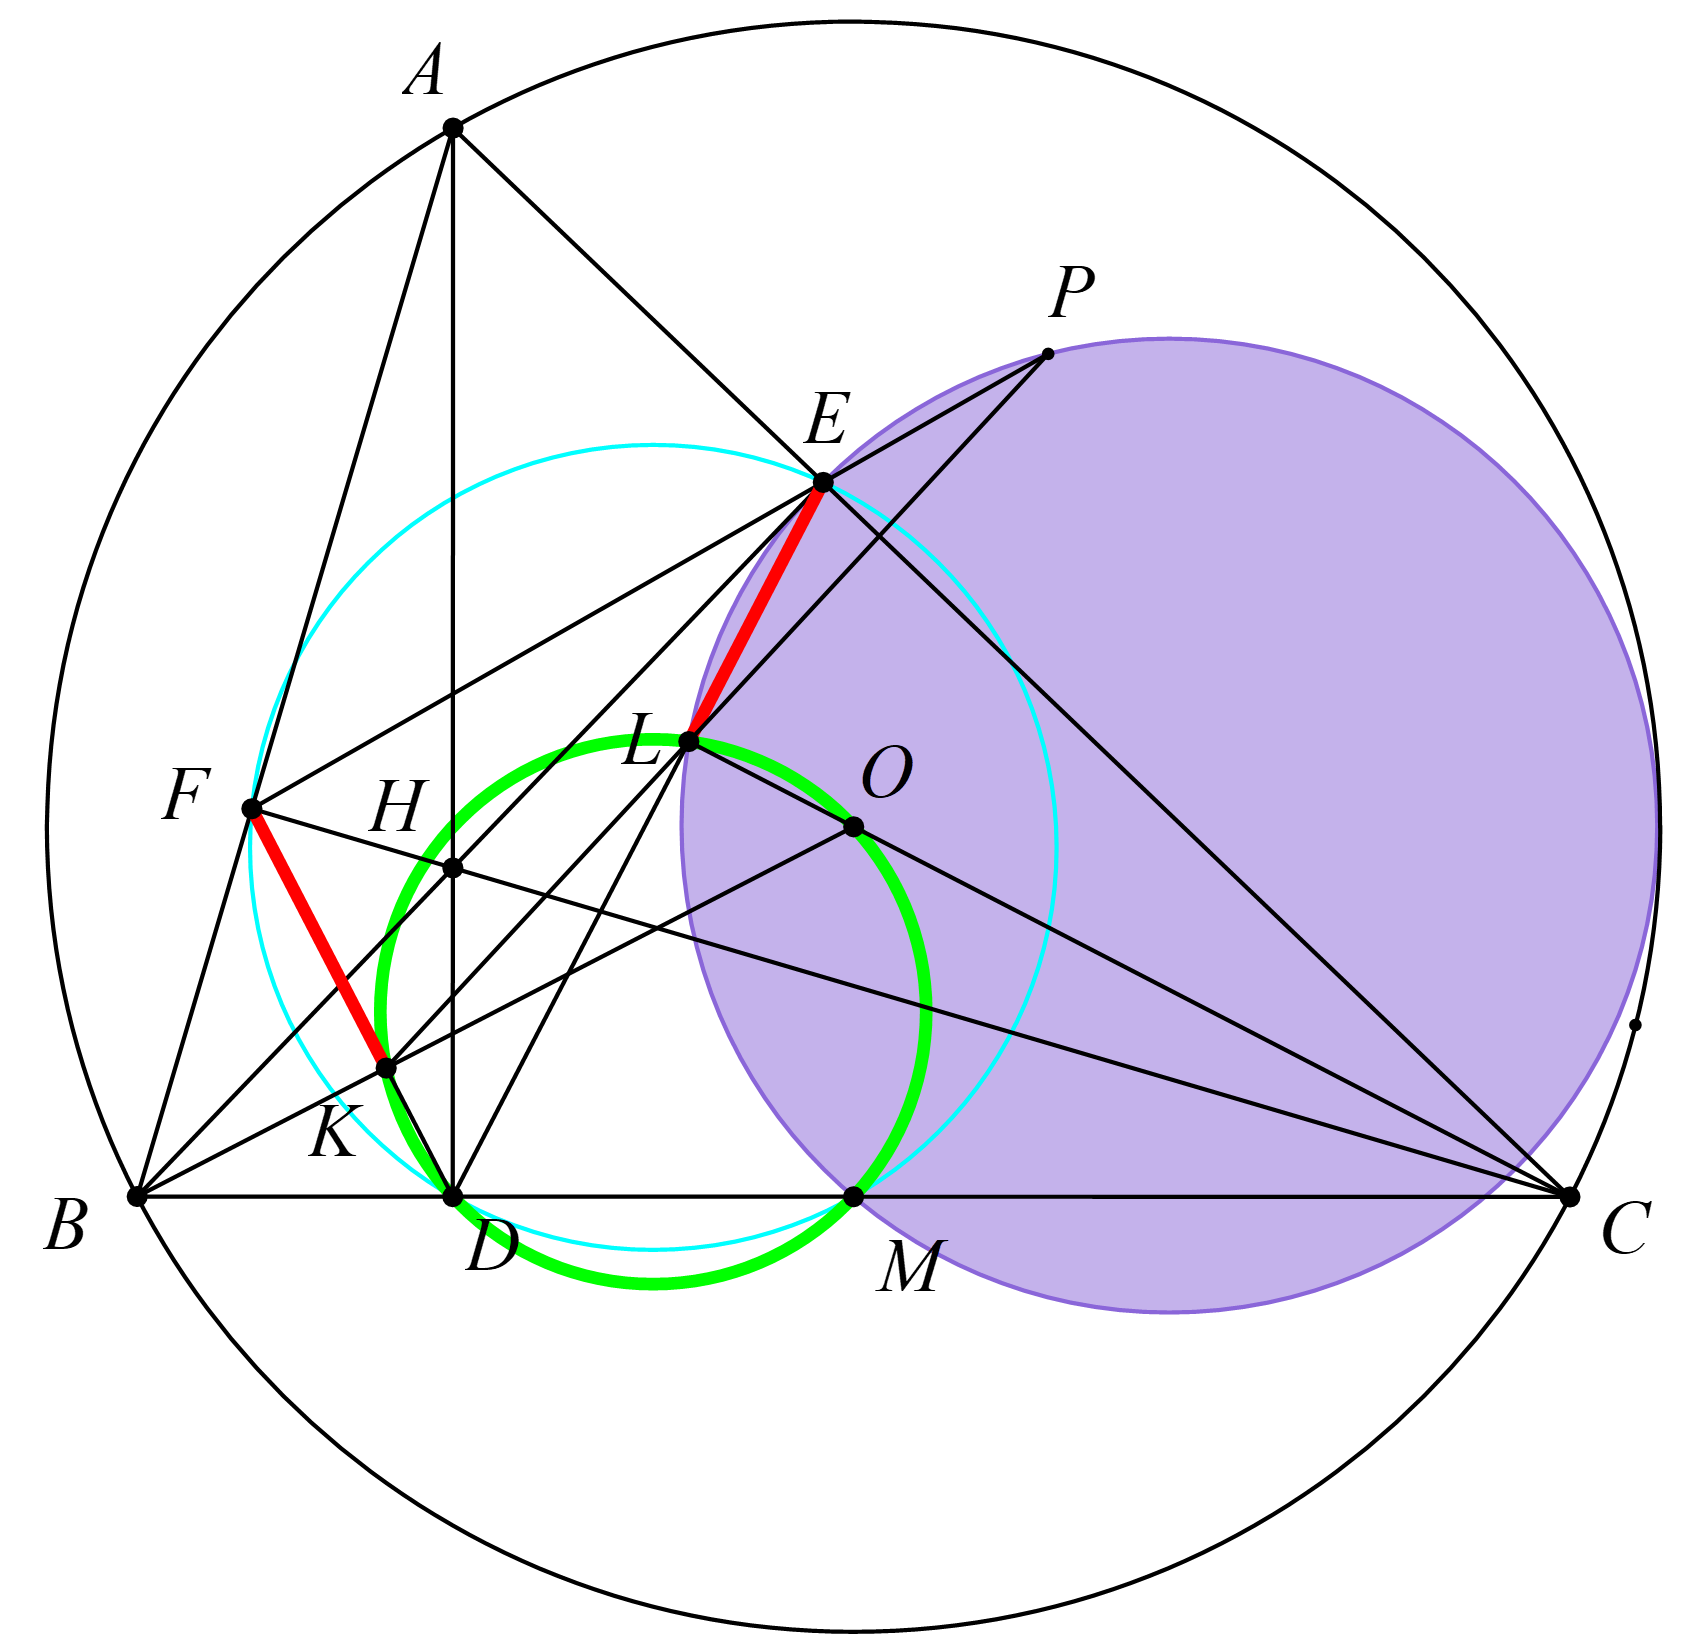
\includegraphics[width= 1\linewidth]{16}
		\vspace*{-10pt}
	\end{figure}
	\textit{Lời giải.} Vì $BH, BO$ đẳng giác trong góc $B$ nên $BO$ vuông góc với $FD$. Tương tự, $CO$ vuông góc với $ED$. Để ý rằng $B,C$ tương ứng là tâm các đường tròn bàng tiếp góc $E,F$ của tam giác $DEF$ nên ta dễ chứng minh được $KF=LE$. Gọi $M$ là trung điểm $BC$. Dễ thấy $ME=MF$ nên $M$ là trung điểm của cung $FE$ chứa $D$ của đường tròn $(FDE)$, đường tròn Euler của tam giác $ABC$. Do đó theo Bổ đề $1$ thì $M$ là điểm Miquel của tứ giác toàn phần $EFKLDP$. Vì thế đường tròn $(LEP)$ luôn qua điểm $M$ cố định khi $A$ di động trên $O$.
	\vskip 0.1cm
	Bài toán sau đây do tác giả Trần Quang Hùng đề xuất.
	\vskip 0.1cm
	\textbf{\color{hoccungpi}Ví dụ $\pmb{9.}$} Cho tam giác $ABC$. Các điểm $E,F$ tương ứng thay đổi trên $AC,AB$ sao cho $CE=BF$. Chứng minh rằng đường thẳng Euler của tam giác $AEF$ luôn đi qua một điểm cố định.
	\vskip 0.1cm
	\textit{Phân tích.} Rõ ràng bài toán này có mô hình hai đoạn thẳng bằng nhau là $CE=BF$ nên ta có thể vận dụng Bổ đề $1$ để tiếp cận. Theo Bổ đề $1$ thì hai đường tròn $(AEF)$ và $(ABC)$ cắt nhau tại trung điểm cung của mỗi đường tròn, từ đó ta có thêm thông tin để giải bài toán.
	\vskip 0.1cm
	\textit{Lời giải.} Gọi $ G,L$ tương ứng là trọng tâm các tam giác $ABC,AEF$. Gọi $(O)$ và $(K)$ tương ứng là các đường tròn ngoại tiếp các tam giác $ABC, AEF$. Khi đó $LK,GO$ tương ứng là đường thẳng Euler của các tam giác $AEF,ABC$. Gọi giao điểm của $LK$ và $ GO$ là $R$. Ta sẽ chứng minh $R$ là một điểm cố định. Thật vậy, theo Bổ đề $1$ thì $(O)$ và $(K)$ cắt nhau tại $T$ trên các đường trung trực $EF,BC$. Gọi $ M,N$ tương ứng là trung điểm của các đoạn thẳng $BC,EF$. Ta thấy rằng các tam giác cân $TEF,TBC$ đồng dạng, do đó ta suy ra được $\dfrac{TK}{TN} = \dfrac{KO}{MN} = \dfrac{TO}{TM}$, là tỷ số không đổi.
	\begin{figure}[H]
		\vspace*{-5pt}
		\centering
		\captionsetup{labelformat= empty, justification=centering}
		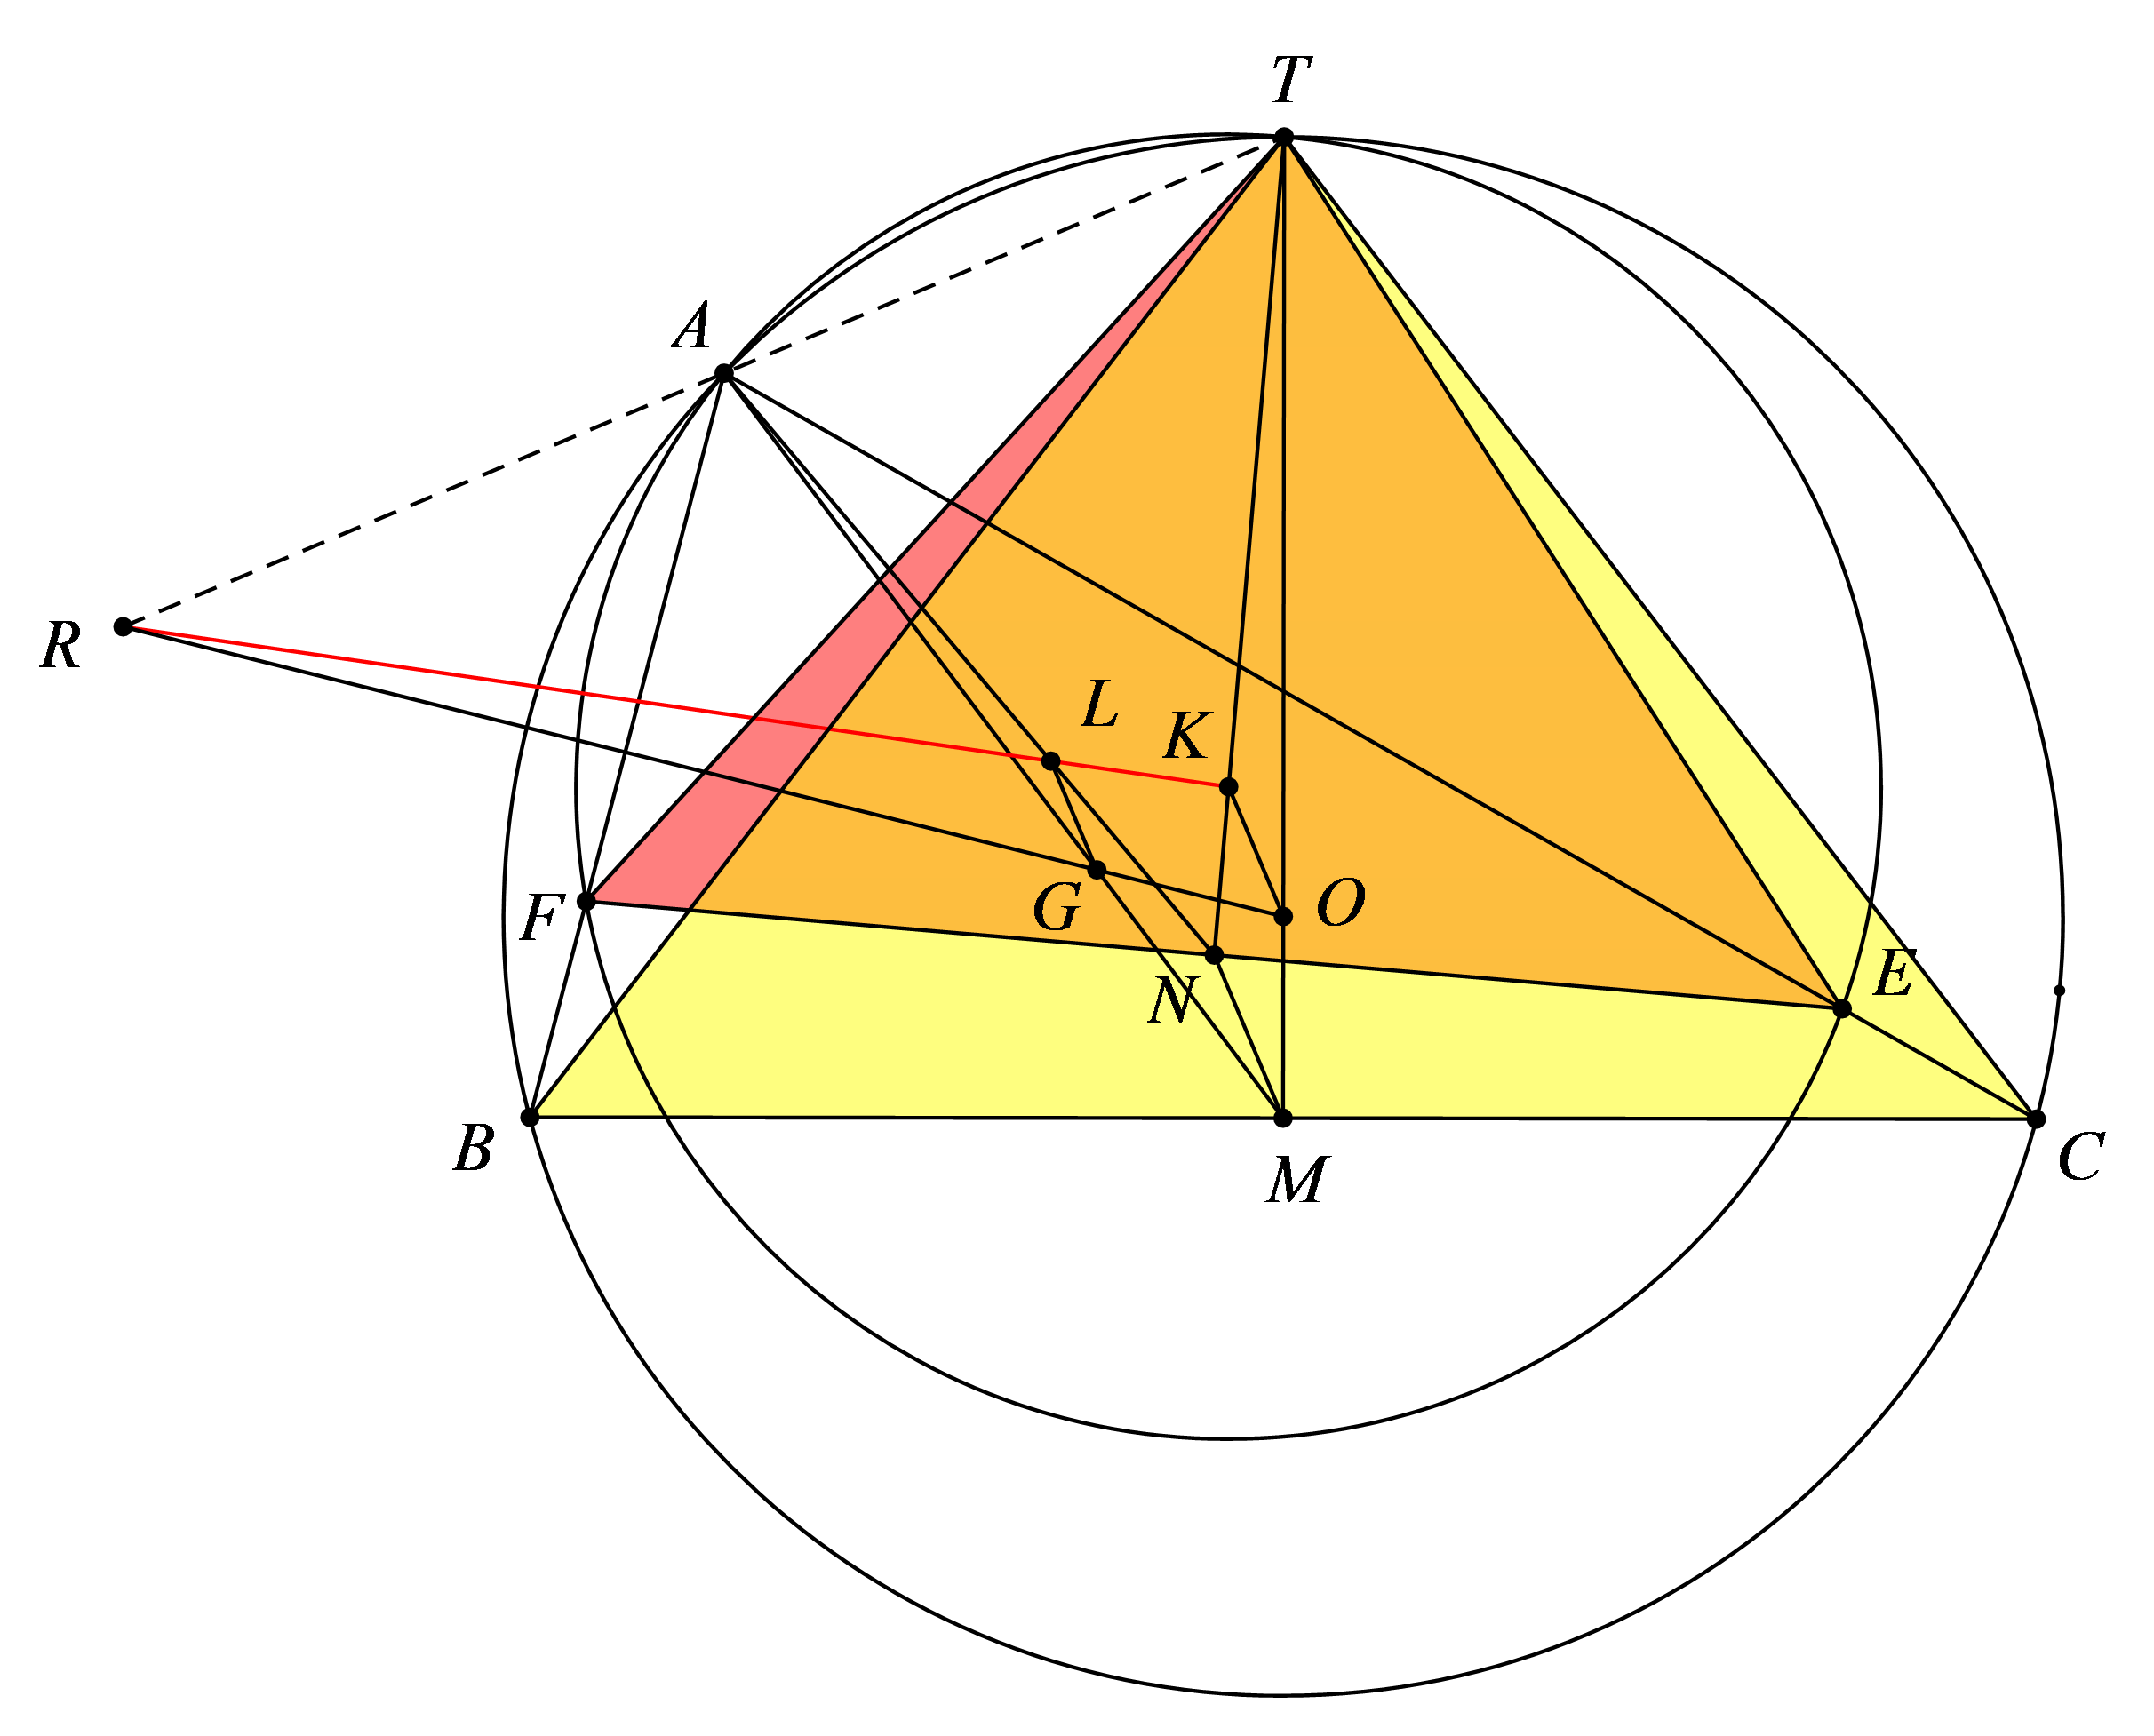
\includegraphics[width= 1\linewidth]{17}
		\vspace*{-10pt}
	\end{figure}
	Suy ra $MN\parallel KO$. Ta lại có $\dfrac{GL}{MN} = \dfrac{2}{3}$  và $GL\parallel MN$, do đó $GL\parallel KO$ và
	\begin{align*}
		\dfrac{GL}{KO} = \dfrac{GL}{MN}\cdot \frac{MN}{KO} = \dfrac{2}{3} \cdot \dfrac{TM}{TO}.
	\end{align*}
	Từ đó, tỷ số $\dfrac{RG}{RO} = \dfrac{GL}{KO}$ là không đổi, do đó điểm $R$ là cố định. Vậy $KL$ luôn đi qua điểm $R$ cố định.
	\vskip 0.1cm
	$\pmb{2.4.}$ \textbf{\color{hoccungpi}Chứng minh nhiều đường tròn đồng quy}
	\vskip 0.1cm
	Bài toán sau đây xuất hiện trong đề thi Olympic Toán quốc gia của Mỹ năm $2006$.
	\vskip 0.1cm
	\textbf{\color{hoccungpi}Ví dụ $\pmb{10.}$}  Cho tứ giác lồi $ABCD$ có các cặp cạnh đối không song song và $E,F$ lần lượt là các điểm trên các cạnh $AD$ và $BC$ sao cho  $\dfrac{AE}{ED} = \dfrac{BF}{FC}$, $EF$ cắt $AB,CD$ lần lượt tại $S,T$. Chứng minh các đường tròn $(SAE)$, $(SBF)$, $(TCF)$, $(TDE)$ cùng đi qua một điểm.
	\vskip 0.1cm
	\textit{Phân tích.} Đề bài cho tứ giác toàn phần $ABCD$ và các điểm $E,F$ lần lượt chia các đoạn $AD,BC$ theo cùng tỷ số nên ta có thể liên tưởng đến mô hình hai đoạn thẳng. Hơn nữa, yêu cầu bài toán là chứng minh các đường tròn đồng quy nên ta có thể nghĩ đến điểm Miquel của tứ giác toàn phần, cũng chính là tâm của phép vị tự quay trong Bổ đề $2$.
	\begin{figure}[H]
		\vspace*{-5pt}
		\centering
		\captionsetup{labelformat= empty, justification=centering}
		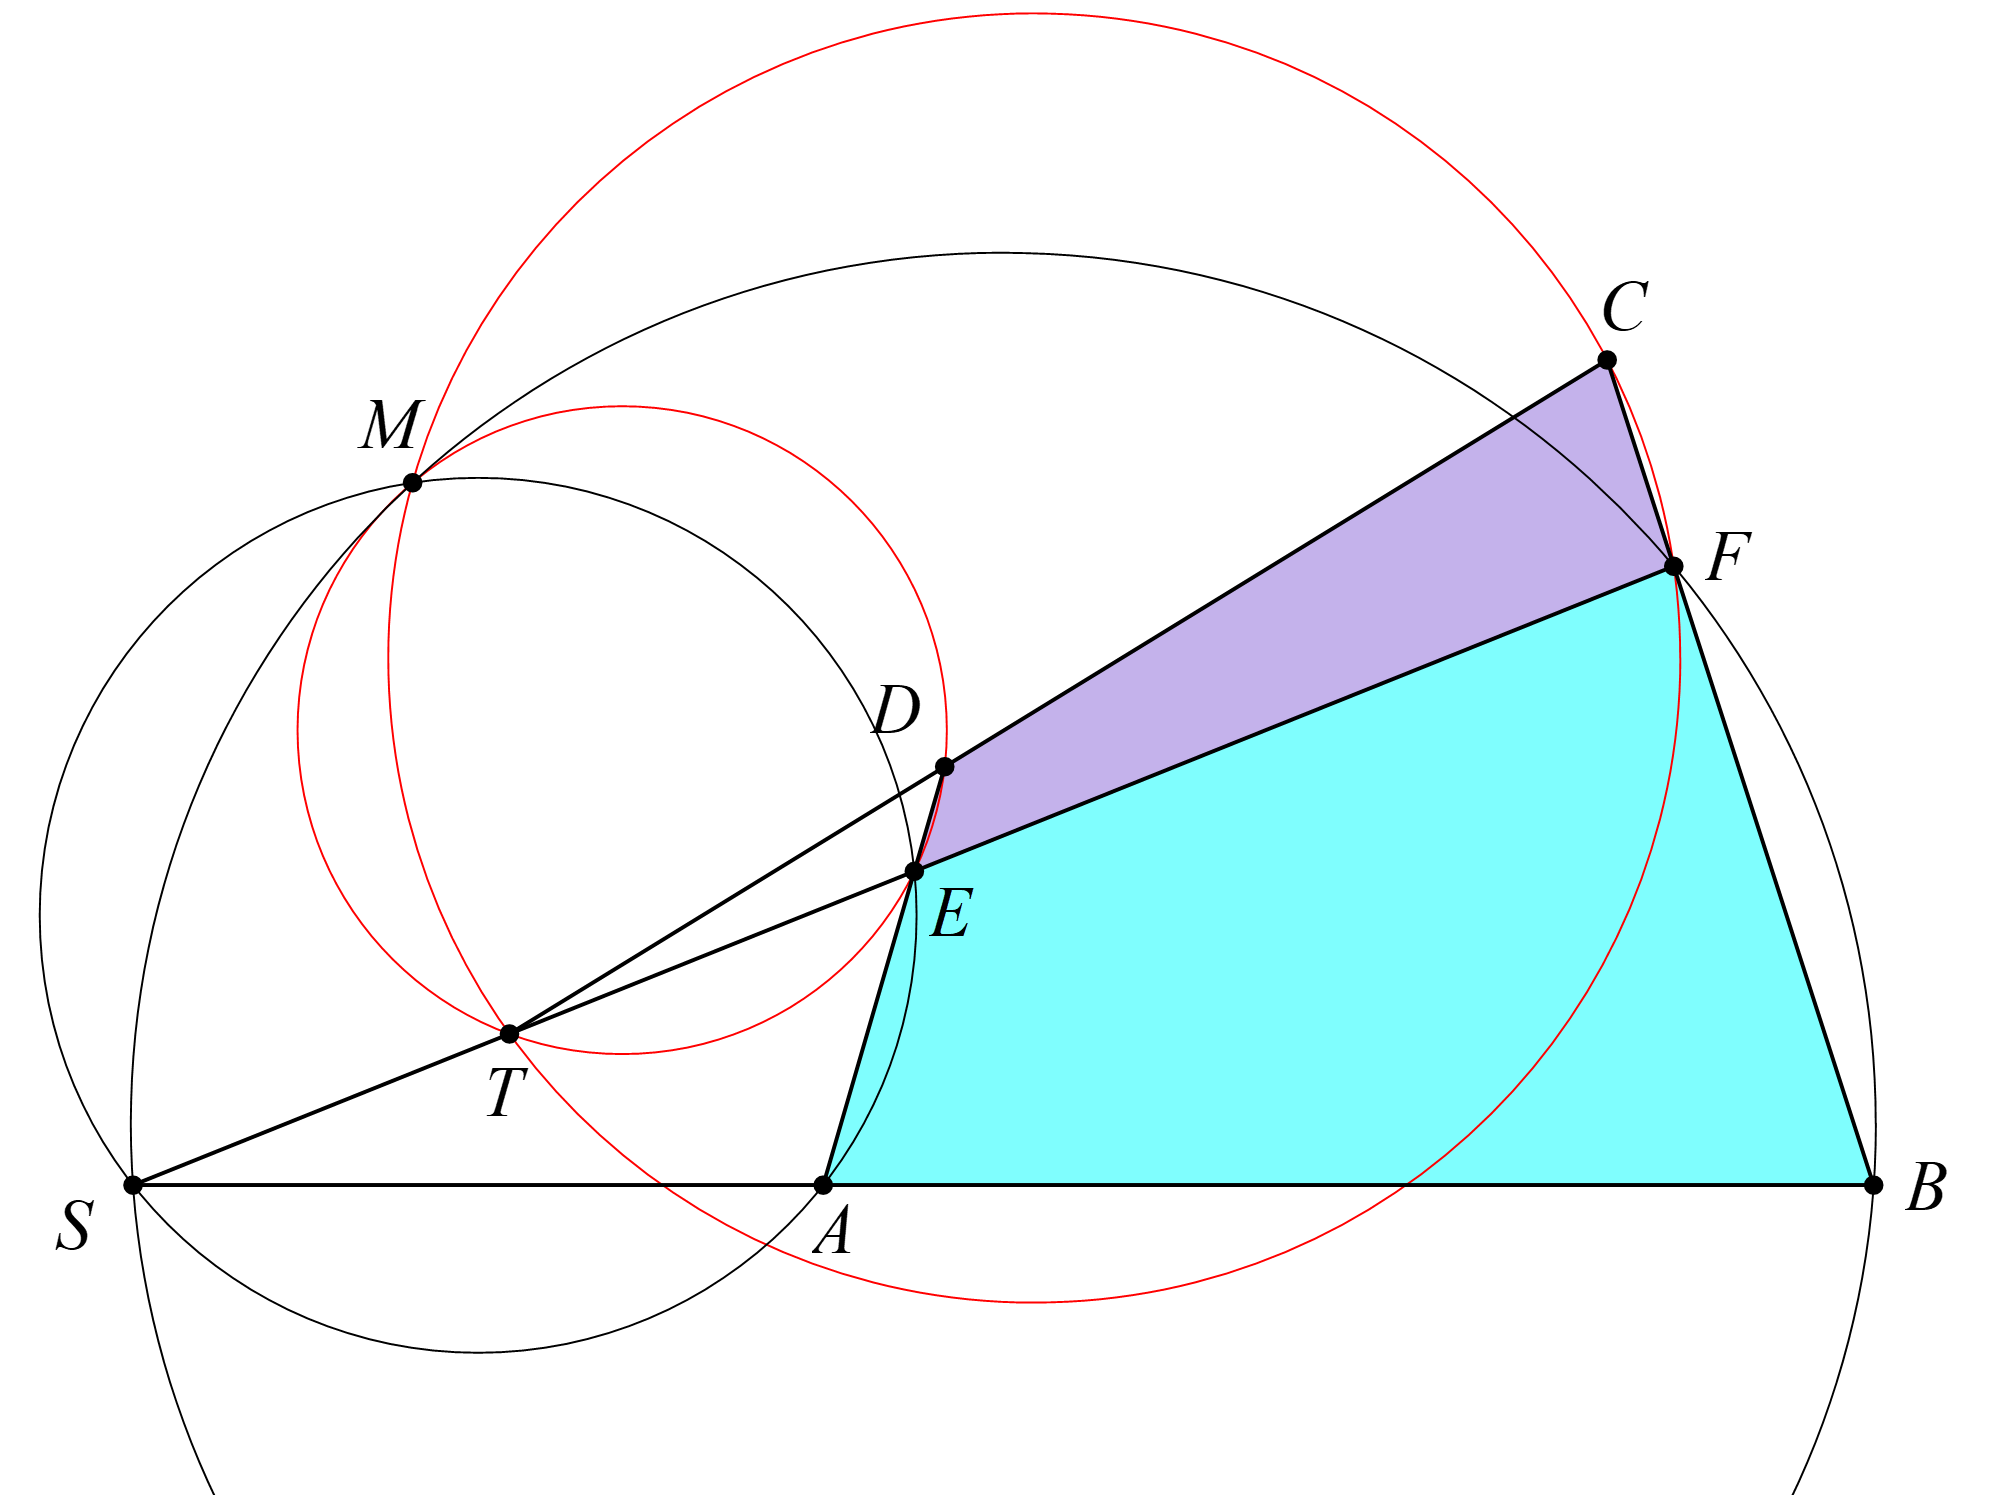
\includegraphics[width= 1\linewidth]{18}
		\vspace*{-10pt}
	\end{figure}
	\textit{Lời giải.} Gọi $M$ là tâm của phép vị tự quay $f$ biến $A$ thành $B$, biến $D$ thành $C$, do đó biến $AD$ thành $BC$. Vì các điểm $E,F$ chia các đoạn thẳng này theo cùng tỷ số nên phép vị tự quay này cũng biến $E$ thành $F$. Do đó $f$ biến $AE$ thành $BF$ và biến $ED$ thành $FC$. Như vậy, tâm $M$ là điểm Miquel chung của các tứ giác toàn phần $ABFE$ và $EFCD$ (cũng như tứ giác $ABCD$). Vậy, các đường tròn $(SAE)$, $(SBF)$, $(TCF)$, $(TDE)$ cùng đi qua điểm Miquel $M$.
	\begin{figure}[H]
		%		\vspace*{-5pt}
		\centering
		\captionsetup{labelformat= empty, justification=centering}
		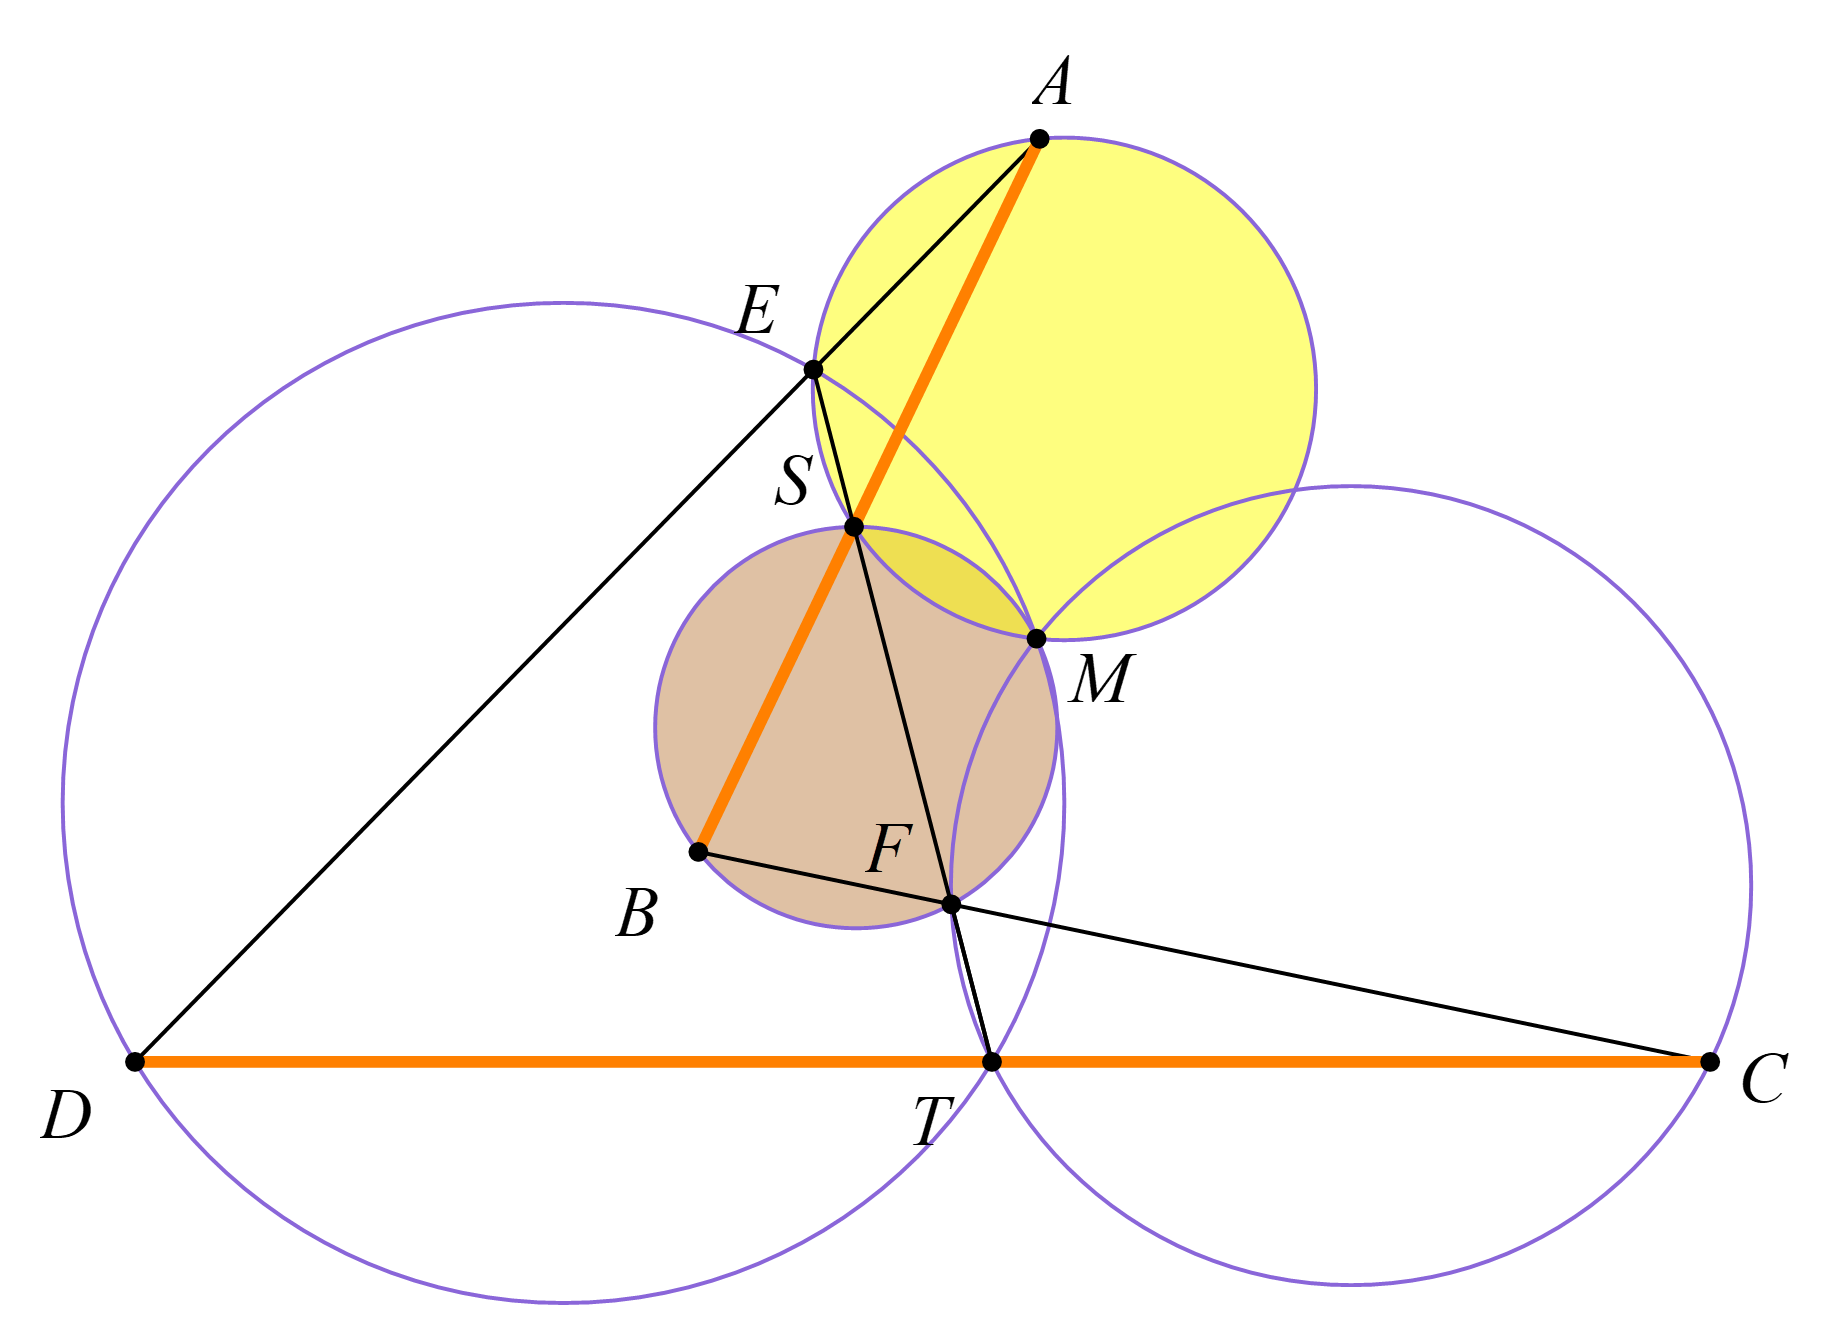
\includegraphics[width= 1\linewidth]{19}
		\vspace*{-10pt}
	\end{figure}
	\textit{Nhận xét:} Nếu thay giả thiết tứ giác $ABCD$ lồi bởi bốn điểm $A,B,C,D$ bất kỳ thì ta cũng thu được kết quả tương tự.
	\vskip 0.1cm
	$\pmb{2.5.}$ \textbf{\color{hoccungpi}Một số bài tập}
	\vskip 0.1cm
	Để kết thúc bài viết, chúng tôi xin mời độc giả thử sức mình với một số bài toán mà lời giải có thể sử dụng các Bổ đề $1$ và $2$.
	\vskip 0.1cm
	\textbf{\color{hoccungpi}Bài $\pmb{1}$ (Chọn đội tuyển Mỹ năm $\pmb{2007}$).} Hai đường tròn $(O)$ và $(O')$ cắt nhau tại $P,Q$.  Qua $P$ vẽ hai cát tuyến $PAB$ và $PCD$ sao cho $A,C$ thuộc $(O)$ và $B,D$ thuộc $(O')$. Tia $BD$ cắt đoạn $AC$ tại $X$. Lấy điểm $Y$ thuộc $(O)$ và $Z$ thuộc $(O')$ sao cho $PY\parallel BD,PZ\parallel AC$. Chứng minh $Q,X,Y,Z$ thẳng hàng.
	\vskip 0.1cm
	\textbf{\color{hoccungpi}Bài $\pmb{2}$.} Cho tam giác $ABC$, các điểm $E,F$ di chuyển trên $AC,AB$ sao cho $CE=BF$. Chứng minh rằng tâm đường tròn Euler của tam giác $AEF$ luôn thuộc một đường thẳng cố định khi $E,F$ di chuyển.
	\vskip 0.1cm
	\textbf{\color{hoccungpi}Bài $\pmb{3}$.} Cho tam giác $ABC$ có trung tuyến $AM$. Gọi $I,J$ lần lượt là tâm các đường tròn $(AMB),(AMC),O$ là tâm đường tròn $(ABC)$. Chứng minh $AO$ là đường đối trung của tam giác $AIJ$.
	\vskip 0.1cm
	\textbf{\color{hoccungpi}Bài $\pmb{4}$ (Olympic Iran $\pmb{1997}$).} Cho tam giác ABC nội tiếp đường tròn $(O)$. Điểm $P$ di chuyển trên cung $BC$ không chứa $A$, gọi $I,J$ lần lượt là tâm nội tiếp các tam giác $APB,APC$. Chứng minh đường tròn $(PIJ)$ luôn đi qua một điểm cố định.
	\vskip 0.1cm
	\textbf{\color{hoccungpi}Bài $\pmb{5}$.} Cho hai đường tròn $(O)$ và $(O')$ cắt nhau  tại $A,B$. Một cát tuyến thay đổi qua $A$ cắt $(O),(O')$ lần lượt tại $D,E$. Tiếp tuyến của $(O)$ tại $D$ và tiếp tuyến của $(O')$ tại $E$ cắt nhau tại $P$. Chứng minh rằng trung trực của đoạn $BP$ luôn tiếp xúc với một đường tròn cố định.
	\vskip 0.1cm
	\textbf{\color{hoccungpi}Bài $\pmb{6}$ (Olympic Canada $\pmb{2013}$).} Cho tam giác $ABC$ vuông tại $C$ có trọng tâm $G$, gọi $P$ là điểm trên $AG$ sao cho  $\angle CPA = \angle CAB$, $Q$ là điểm trên $BG$ sao cho  $\angle CQB = \angle ABC$. Chứng minh rằng các đường tròn $(AQG)$ và $(BPG)$ cắt nhau tại một điểm thuộc cạnh $AB$.
	\vskip 0.1cm
	\textbf{\color{hoccungpi}Bài $\pmb{7}$.} Cho tam giác $ABC$ nhọn có trực tâm $H$ và nội tiếp đường tròn $(O)$. Trung trực $AH$ cắt $AB,AC$ lần lượt tại $D,E$. Chứng minh rằng $OA$ là phân giác của góc  $\angle DOE$.
	\vskip 0.1cm
	\textbf{\color{hoccungpi}Bài $\pmb{8}$ (Olympic Trung Quốc $\pmb{1992}$).} Cho tứ giác lồi $ABCD$ nội tiếp đường tròn $(O),AC$ cắt $BD$ tại $P$, các đường tròn $(PAB)$ và $(PCD)$ cắt nhau tại $Q$ khác $P$ và $O$. Chứng minh $QO$ vuông góc với $QP$.
	\vskip 0.1cm
	\textbf{\color{hoccungpi}Bài $\pmb{9}$ (Olympic Toán quốc tế $\pmb{2004}$).} Cho tứ giác lồi $ABCD$, đường chéo $BD$ không là phân giác các góc  $\angle ABC, \angle CDA$. Điểm $P$ nằm trong tứ giác sao cho  $\angle PBC = \angle DBA, \angle DBC = \angle BDA$. Chứng minh tứ giác $ABCD$ nội tiếp được khi và chỉ khi $PA=PC$.
	\vskip 0.1cm
	\textbf{\color{hoccungpi}Bài $\pmb{10}$.} Cho tam giác $ABC$ nội tiếp đường tròn $(O),N$ là trung điểm cung $BC$ chứa $A$ của $(O), M$ là một điểm bất kỳ trên trung trực đoạn $BC$. Gọi $I,J$ lần lượt là tâm đường tròn bàng tiếp góc $A$ của các tam giác $ABM,ACM$. Chứng minh $I,J,A,N$ đồng viên.
	\vskip 0.1cm
	\textbf{\color{hoccungpi}Tài liệu tham khảo}
	\vskip 0.1cm
	[$1$] Lê Bá Khánh Trình, \textit{Hình học tĩnh và động}, tạp chí Pi, số $8$, tháng $8/2019$. 
	\vskip 0.1cm
	[$2$] Trần Quang Hùng. \textit{Ứng dụng một số bổ quen thuộc vào các bài toán hình học thi Olympic}.
	\vskip 0.1cm
	[$3$] Nguyễn Minh Hà, Nguyễn Xuân Bình, \textit{Bài tập nâng cao và một số chuyên đề Hình học $10$}, NXB Giáo dục, $2008$.
	\vskip 0.1cm
	[$4$] Nguyễn Văn Ban, Hoàng Chúng, \textit{Hình học của tam giác}, NXB Giáo dục.
	\vskip 0.1cm
	[$5$] V.V. Praxolov, \textit{Các bài toán về hình học phẳng, Tập II}, NXB Hải Phòng, $2002$.
	\vskip 0.1cm
	[$6$] Johnson, A. R, \textit{Advanced Euclidean Geometry}, Publications, Inc, Mineola, New York, $2007$.
\end{multicols}

